\section{Calibration and validation of the thermodynamic potentials}


This section presents the calibration results for various types of neural network-based thermodynamic potentials, namely $\Psi_{nn}$, $e_{nn}$, $\Gamma_{nn}$ and $\Upsilon_{nn}$, calibrated according to both calibration strategies described in Sections \ref{sec:strategy 1} and \ref{sec:strategy 2}.

\subsection{Calibration strategy 1}

 We begin showing the calibration results by using Sobolev-type calibration strategy 1. 

\subsubsection{Neural network architecture's influence: $\Psi_{nn}$ neural network-based ground truth models}

The objective of this preliminary study is to investigate a specific neural network-based thermodynamic potential, namely $\Psi_{nn}(\vect{F},\vect{E}_0,\theta)$. Our focus is to assess how variations in the neural network architecture influence the accuracy of the potential's calibration. The network architecture is characterized by the number of layers, $n_L+1$, and an equal number of neurons per layer, denoted as $n_n$. By varying these parameters, we track the $R^2$ values of the second-order derivatives of the potential--$R^2$ in the derivatives of the potential, namely $R^2(\partial^2_{\vect{F}}\Psi_{nn})$, $R^2(\partial^2_{\vect{E}_0}\Psi_{nn})$ and $R^2(\partial^2_{\theta}\Psi_{nn})$--for both training and testing datasets. It is important to note that the training data, used for calibrating the potential across all architectures, constitutes  $20\%$ of the testing dataset.

Table \ref{table: results calibration strategy 1} shows the results obtained for the calibrated models $\Psi_{nn}$, not only across different neural network architectures but also when employing the various models described in Section  \ref{sec:ground truth models}. These models represent both the purely mechanical and electro-mechanical contributions of the ground truth Helmholtz strain energy model used for the calibration of all the potentials. The results obtained in this table indicate that in general, the optimization algorithm used for the calibration of the models (Adam algorithm with a learning rate of $0.001$) attains a very satisfactory local minimum. 

\begin{table}[hbtp!]
	\centering
	\begin{tabular}{c c c c c c c c }
		\toprule
		\rowcolor{gray!30}	\small{} & $n_L+1$ & 2 &  3& 4& 2& 3& 4\\
		\midrule 
		\rowcolor{gray!30}	\small{} & $n_n$ & 8 & 8& 8 &16& 16& 16\\
		\midrule
		\multirow{3}{*}{\rotatebox{90}{\textcolor{red}{\textbf{MR}}/\textcolor{blue}{\textbf{ID}}}}  &$R^2(\partial_{\vect{F}}\Psi)$ & 0.9994&  0.9999 & 0.9999 & 0.9998 & 0.9999 & 0.9999 \\
		&$R^2(\partial_{\vect{E}_0}\Psi)$ & 0.9999 &  0.9999 & 0.99999 & 0.9999 & 0.9999 & 0.9999\\
		&$R^2(\partial_{\theta}\Psi)$ & 0.9999 & 0.9999 & 0.9999 & 0.9999 & 0.9999 & 0.9999 \\	
		\midrule
		\multirow{3}{*}{\rotatebox{90}{\textcolor{red}{\textbf{QMR}}/\textcolor{blue}{\textbf{ID}}}} &$R^2(\partial_{\vect{F}}\Psi)$ & 0.9989 & 0.9989 & 0.9999 & 0.9999 & 0.9999 & 0.9999 \\
		&$R^2(\partial_{\vect{E}_0}\Psi)$ & 0.9995 & 0.9996 & 0.9999 & 0.9999 & 0.9999 & 0.9999\\
		&$R^2(\partial_{\theta}\Psi)$ & 0.9999 &  0.9999 & 0.99999 & 0.9999 & 0.9999 & 0.9999\\
		\\
		\midrule
		\multirow{3}{*}{\rotatebox{90}{\textcolor{red}{\textbf{Y}}/\textcolor{blue}{\textbf{ID}}}} &$R^2(\partial_{\vect{F}}\Psi)$ & 0.9992 & 0.9999 & 0.9999 & 0.9999 & 0.9999 & 0.9999 \\
&$R^2(\partial_{\vect{E}_0}\Psi)$ & 0.9994 &  0.9999 & 0.9999 & 0.9999 & 0.9999 & 0.9999\\
&$R^2(\partial_{\theta}\Psi)$ & 0.9999 &  0.9999 & 0.99999 & 0.9999 & 0.9999 & 0.9999 \\	
\midrule
		\multirow{3}{*}{\rotatebox{90}{\textcolor{red}{\textbf{G}}/\textcolor{blue}{\textbf{ID}}}} &$R^2(\partial_{\vect{F}}\Psi)$ & 0.9999  & 0.9998 & 0.9998 & 0.9998 & 0.9998 & 0.9999\\
&$R^2(\partial_{\vect{E}_0}\Psi)$ & 0.9999 & 0.9999 & 0.9999 & 0.9999 & 0.9999 & 0.9999\\
&$R^2(\partial_{\theta}\Psi)$ & 0.9999 &  0.9999 & 0.99999 & 0.9999 & 0.9999 & 0.9999\\	
\midrule
		\multirow{3}{*}{\rotatebox{90}{\textcolor{red}{\textbf{TI}}/\textcolor{blue}{\textbf{ID}}}} &$R^2(\partial_{\vect{F}}\Psi)$ & 0.9996 & 0.9996 & 0.9999 & 0.9999&  0.9999&  0.9999\\
&$R^2(\partial_{\vect{E}_0}\Psi)$ &  0.9994 & 0.9992 & 0.9999 & 0.9999 & 0.9999 & 0.9999\\
&$R^2(\partial_{\theta}\Psi)$ & 0.9999 &  0.9999 & 0.99999 & 0.9999 & 0.9999 & 0.9999\\	
\midrule
		\multirow{3}{*}{\rotatebox{90}{\textcolor{red}{\textbf{MR}}/\textcolor{blue}{\textbf{ES}}}} &$R^2(\partial_{\vect{F}}\Psi)$ &  0.9996 &  0.9995 & 0.9995 & 0.9999 & 0.9998 & 0.9999\\
&$R^2(\partial_{\vect{E}_0}\Psi)$ & 0.9998 & 0.9998 & 0.9998 & 0.9999 & 0.9998 & 0.9999\\
&$R^2(\partial_{\theta}\Psi)$ & 0.9999 &  0.9999 & 0.99999 & 0.9999 & 0.9999 & 0.9999 \\	
\midrule
	\end{tabular}
	\caption{\textbf{Calibration Strategy 1}. Values of the $R^2(\partial_{\vect{F}}\Psi)$, $R^2(\partial_{\vect{E}_0}\Psi)$ and $R^2(\partial_{\theta}\Psi)$ obtained in the calibration of $\Psi_{nn}$ (hence using the training dataset) using the purely mechanical (in red) and electro-mechanical (in blue) contributions of the ground truth Helmholtz strain energy model used for the calibration.}
	\label{table: results calibration strategy 1}
\end{table}


Importantly, the calibrated models $\Psi_{nn}(\vect{F},\vect{E}_0,\theta)$ have been evaluated against an independent dataset not included in the original training set. This larger dataset, referred to as the test dataset, has been used to assess the performance of all the ground truth models considered, utilizing a specific neural network architecture. In this study, we have focused on models comprising five layers with eight neurons per layer. The correlation results, presented in Figure \ref{fig:correlation strategy 1},  demonstrate the calibrated models' robust capability to accurately predict the responses of the ground truth models across a significantly broader dataset than the training set.


\begin{figure}[hbtp!]
	\centering
	\begin{tabular}{cccc}
	\rotatebox{90}{\,\,\,\,\,\,\,\,\,\,\textcolor{red}{\textbf{MR}}/\textcolor{blue}{\textbf{ID}}}  &		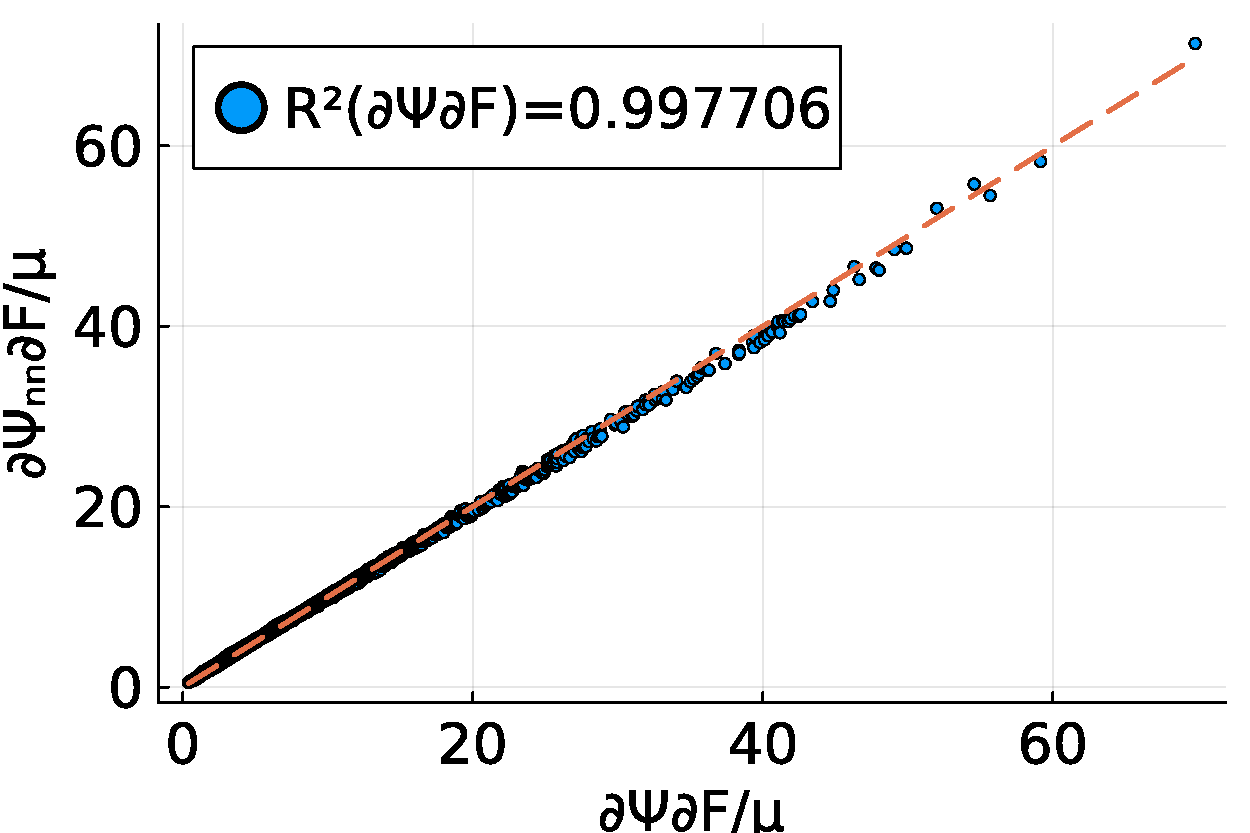
\includegraphics[width=0.3\textwidth]{Figures/ModelsStudy/_MooneyRivlin_ID_E0_P_CorrelationTest} &
		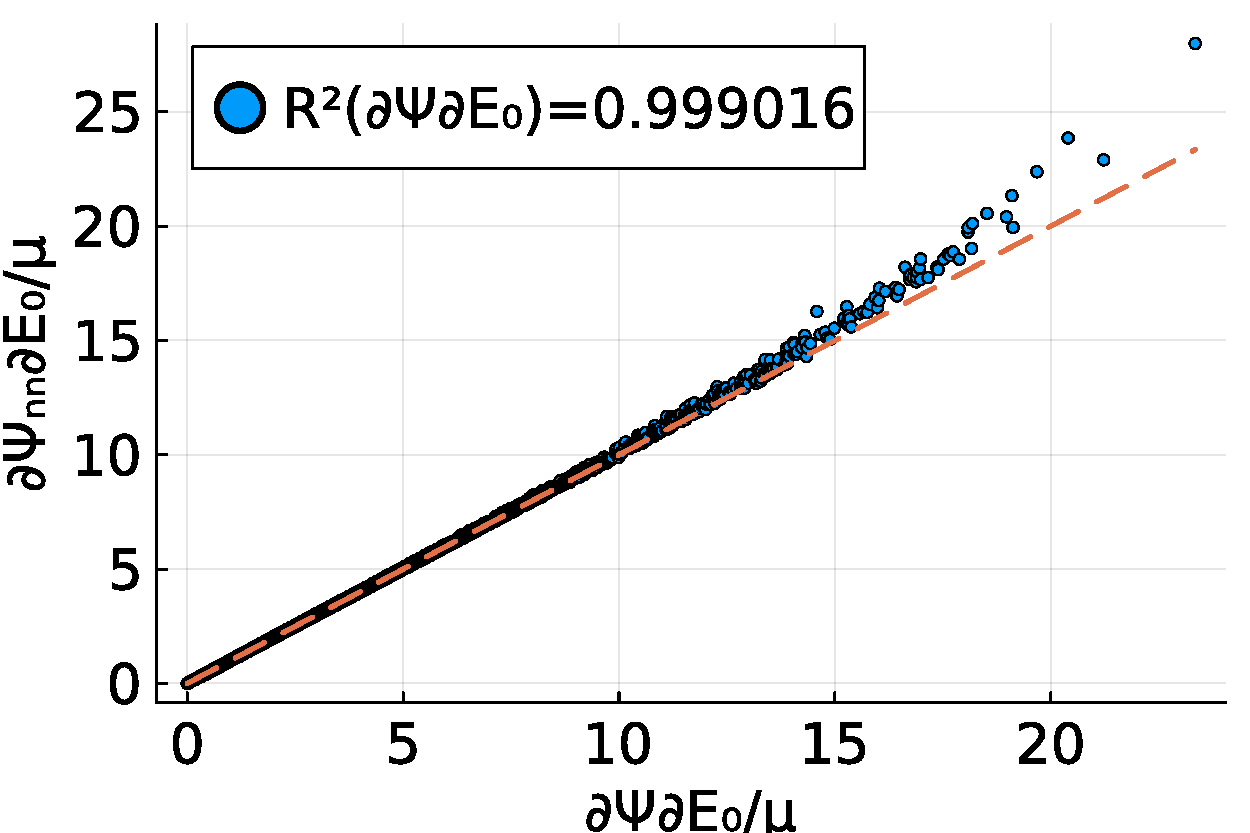
\includegraphics[width=0.3\textwidth]{Figures/ModelsStudy/_MooneyRivlin_ID_E0_E0_CorrelationTest} &
		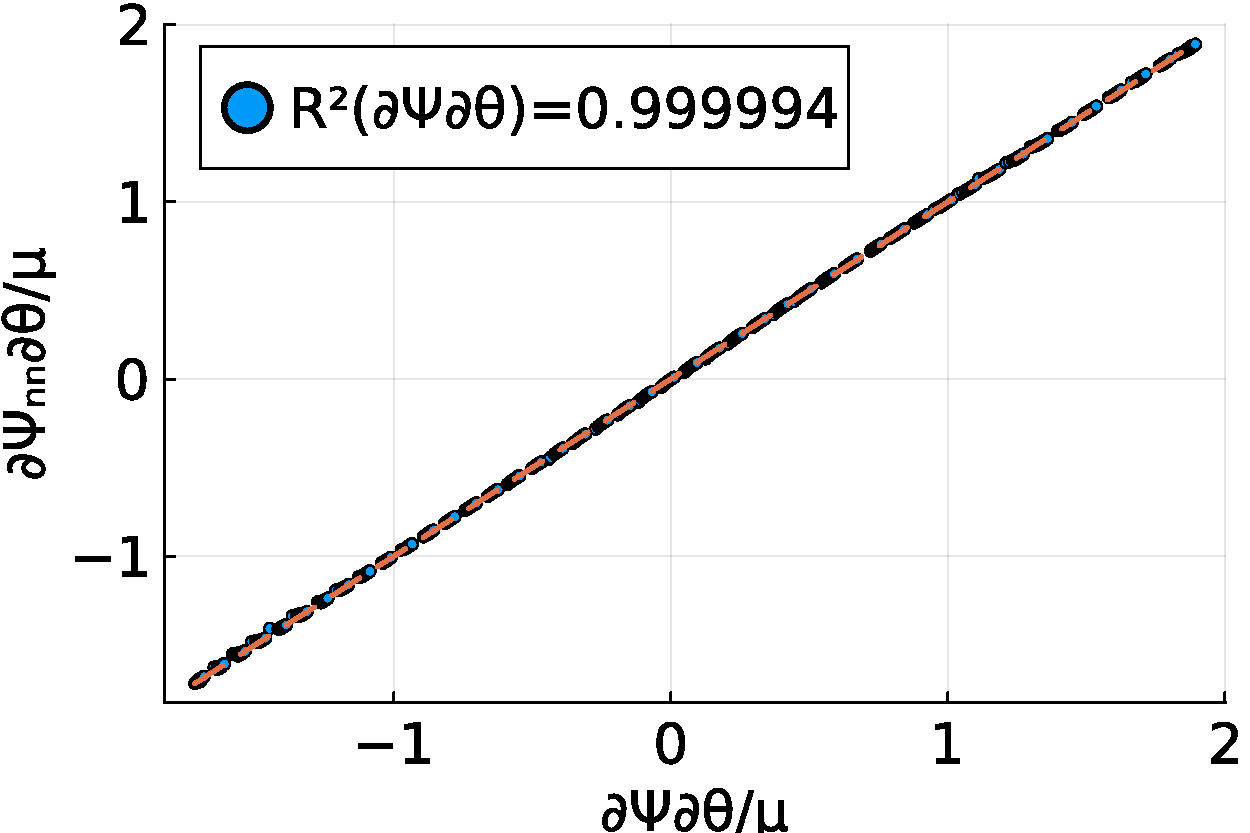
\includegraphics[width=0.3\textwidth]{Figures/ModelsStudy/_MooneyRivlin_ID_E0_theta_CorrelationTest} \\
		%
	\rotatebox{90}{\,\,\,\,\,\,\,\,\,\,\textcolor{red}{\textbf{QMR}}/\textcolor{blue}{\textbf{ID}}} &	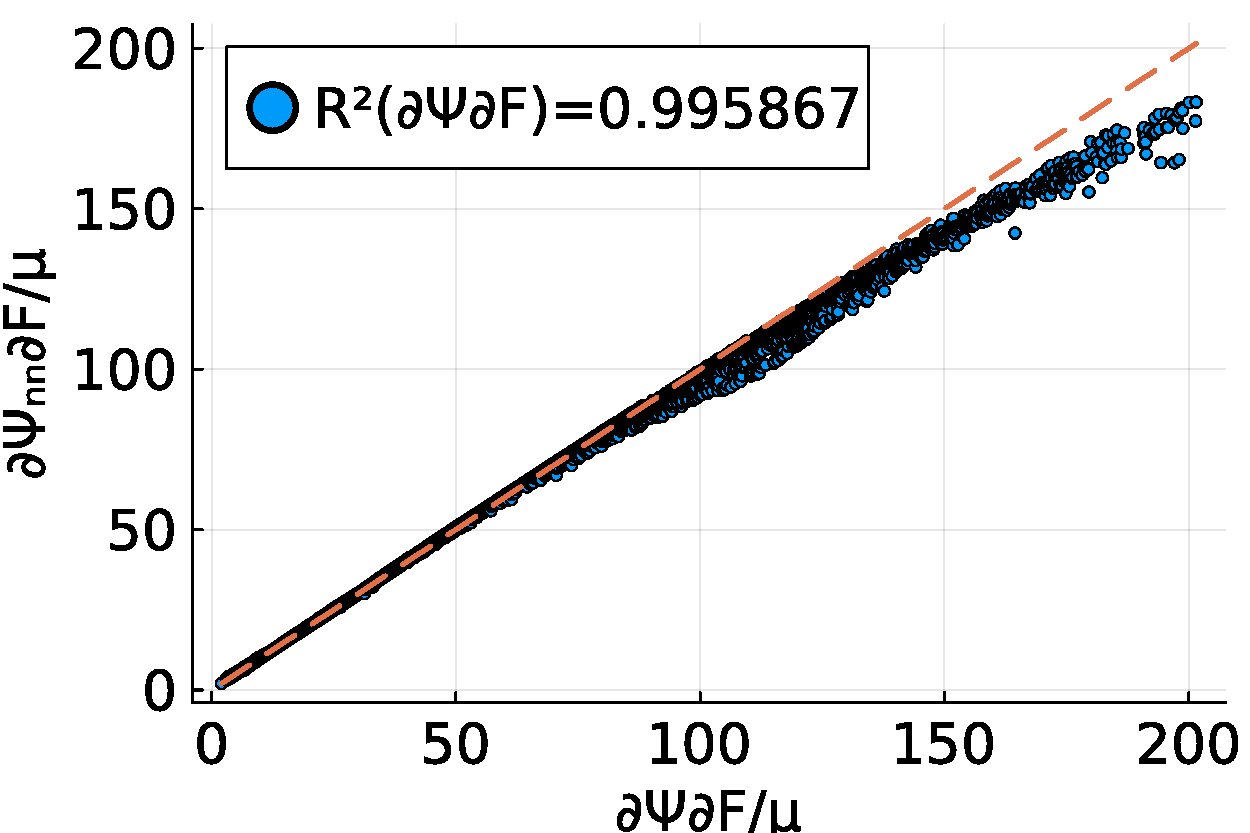
\includegraphics[width=0.3\textwidth]{Figures/ModelsStudy/_QuadraticMooneyRivlin_ID_E0_P_CorrelationTest} &
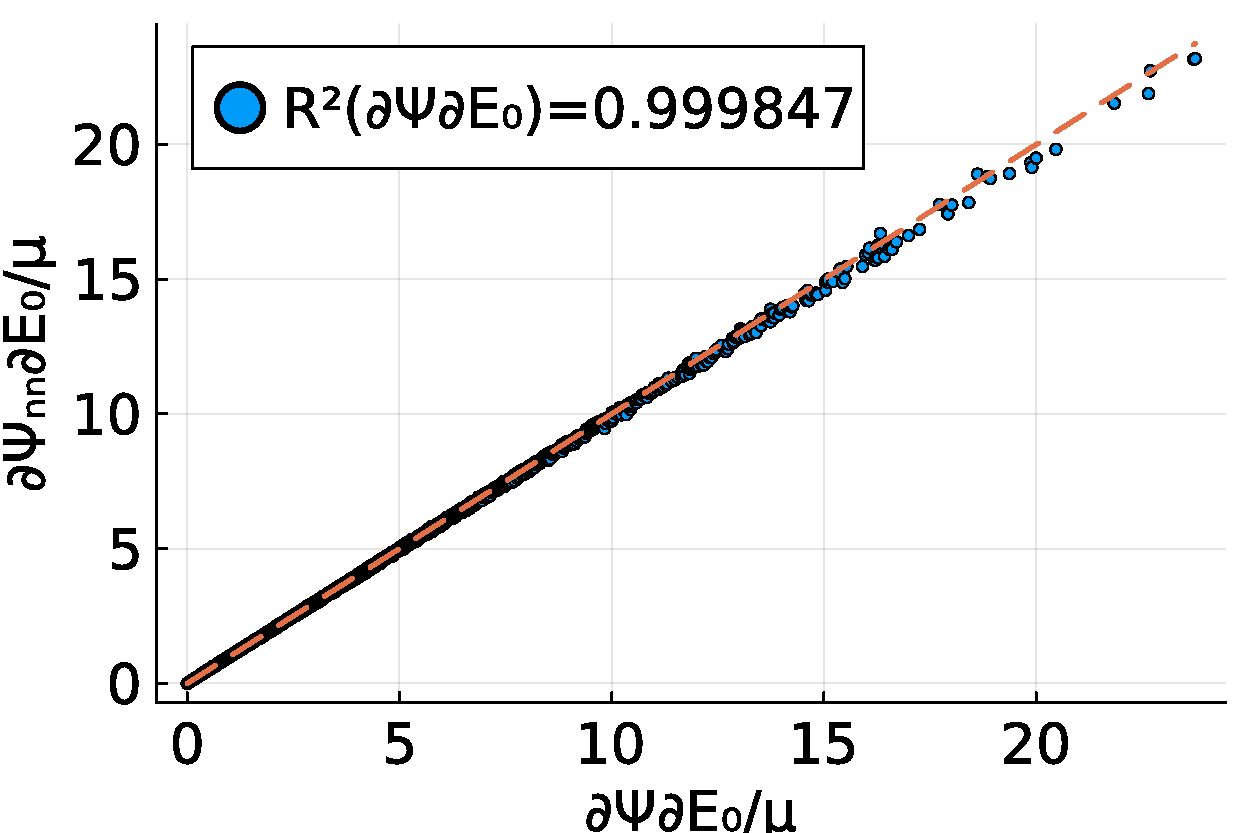
\includegraphics[width=0.3\textwidth]{Figures/ModelsStudy/_QuadraticMooneyRivlin_ID_E0_E0_CorrelationTest} &
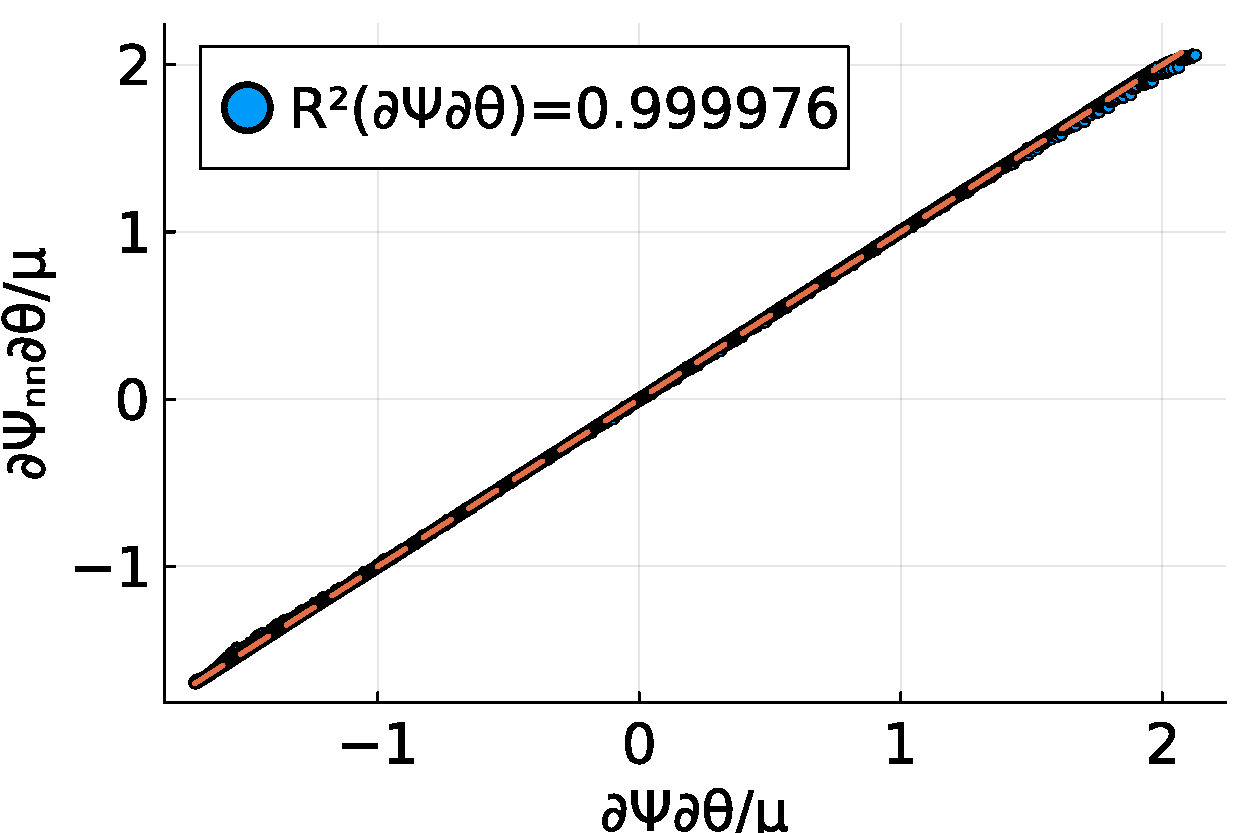
\includegraphics[width=0.3\textwidth]{Figures/ModelsStudy/_QuadraticMooneyRivlin_ID_E0_theta_CorrelationTest} \\
%
%
	\rotatebox{90}{\,\,\,\,\,\,\,\,\,\,\textcolor{red}{\textbf{Y}}/\textcolor{blue}{\textbf{ID}}}  &		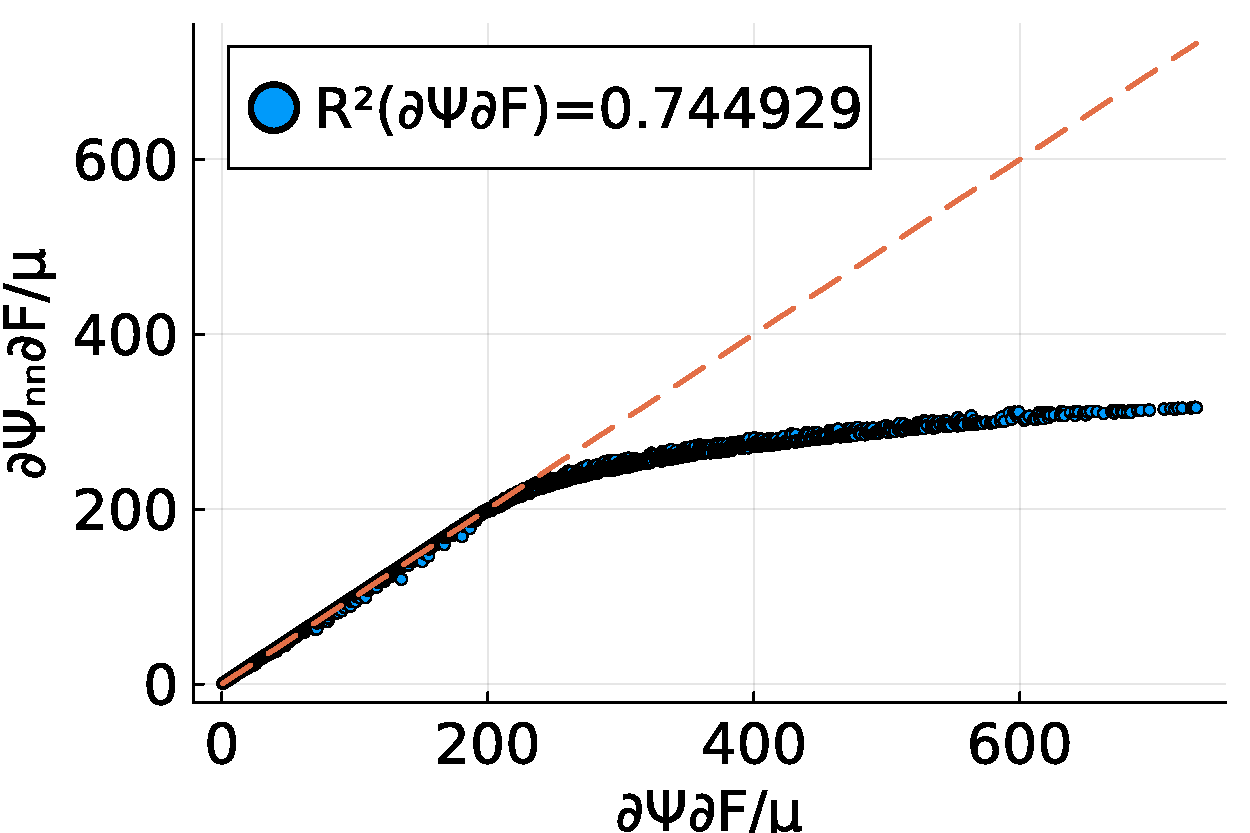
\includegraphics[width=0.3\textwidth]{Figures/ModelsStudy/_Yeoh_ID_E0_P_CorrelationTest} &
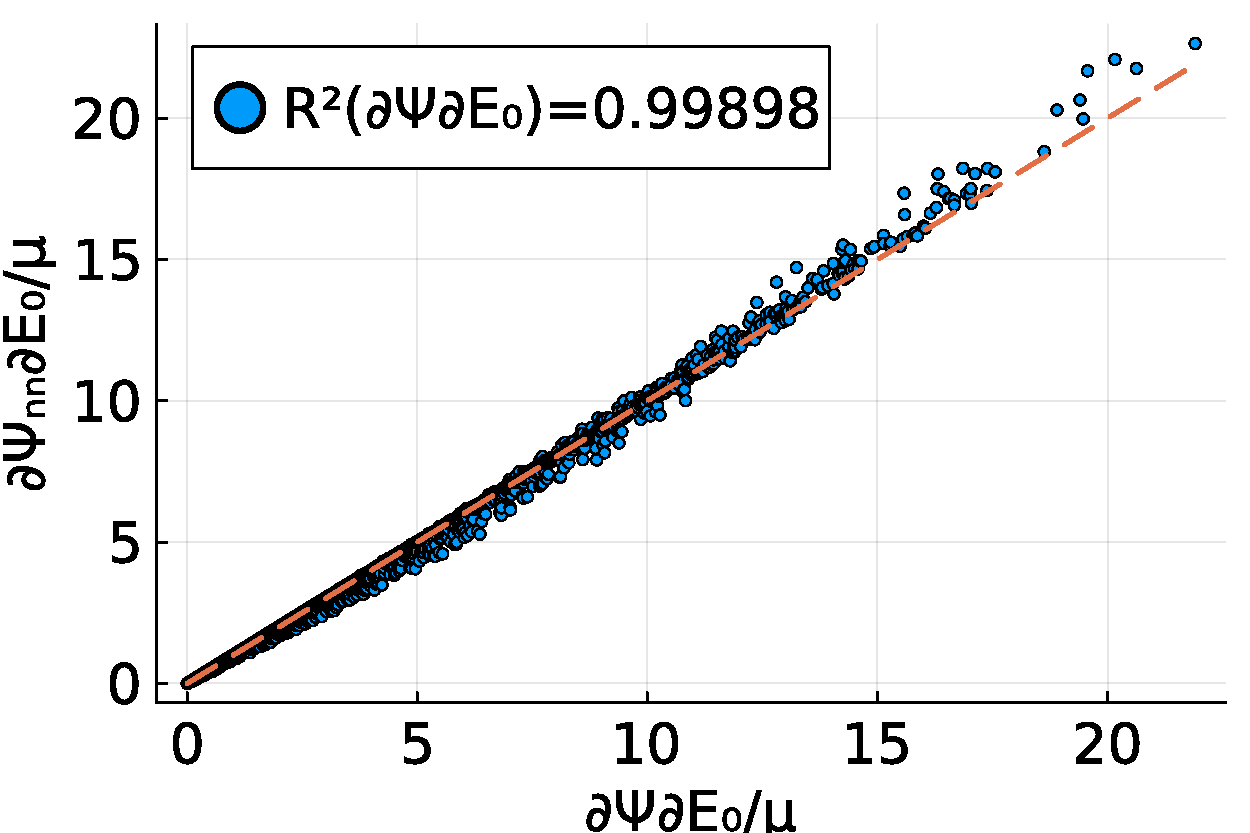
\includegraphics[width=0.3\textwidth]{Figures/ModelsStudy/_Yeoh_ID_E0_E0_CorrelationTest} &
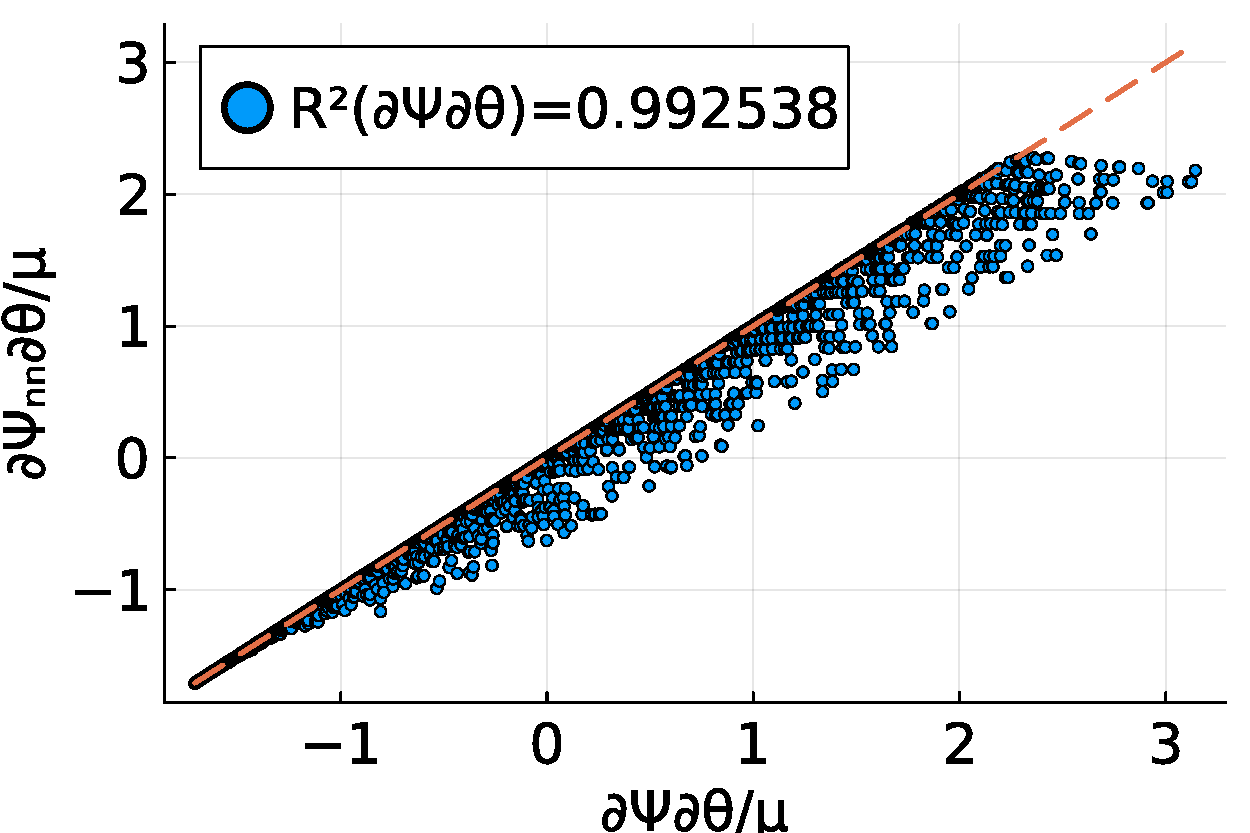
\includegraphics[width=0.3\textwidth]{Figures/ModelsStudy/_Yeoh_ID_E0_theta_CorrelationTest} \\
%
%
	\rotatebox{90}{\,\,\,\,\,\,\,\,\,\,\textcolor{red}{\textbf{G}}/\textcolor{blue}{\textbf{ID}}}  &		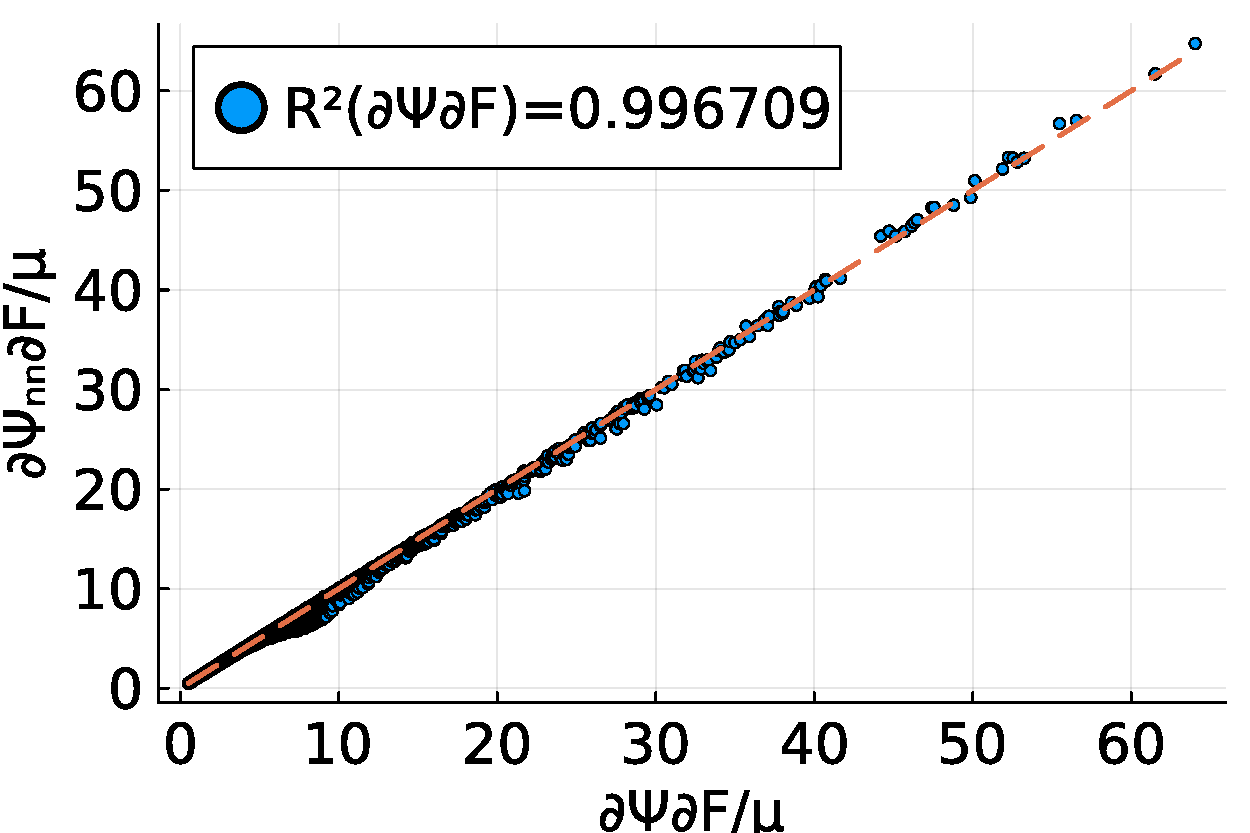
\includegraphics[width=0.3\textwidth]{Figures/ModelsStudy/_Gent_ID_E0_P_CorrelationTest} &
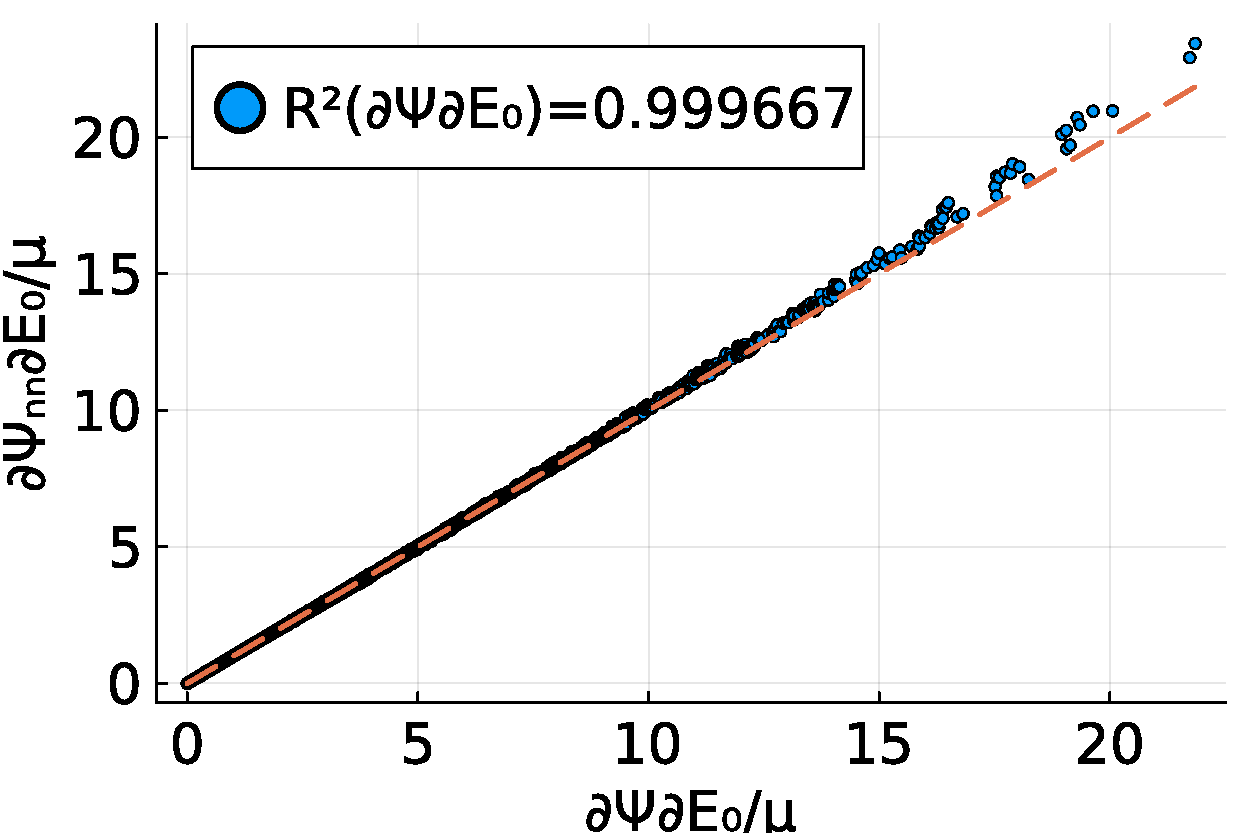
\includegraphics[width=0.3\textwidth]{Figures/ModelsStudy/_Gent_ID_E0_E0_CorrelationTest} &
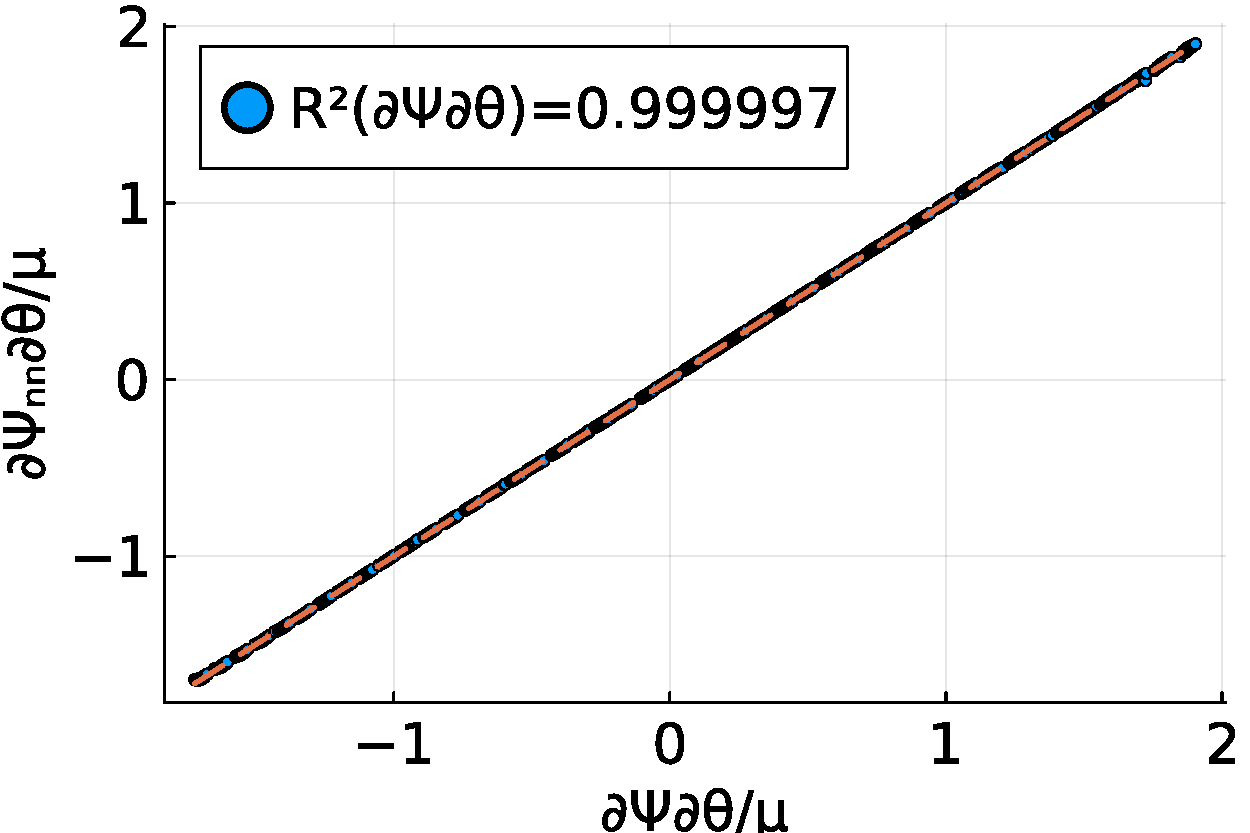
\includegraphics[width=0.3\textwidth]{Figures/ModelsStudy/_Gent_ID_E0_theta_CorrelationTest} \\
%
%
	\rotatebox{90}{\,\,\,\,\,\,\,\,\,\,\textcolor{red}{\textbf{TI}}/\textcolor{blue}{\textbf{ID}}}  &		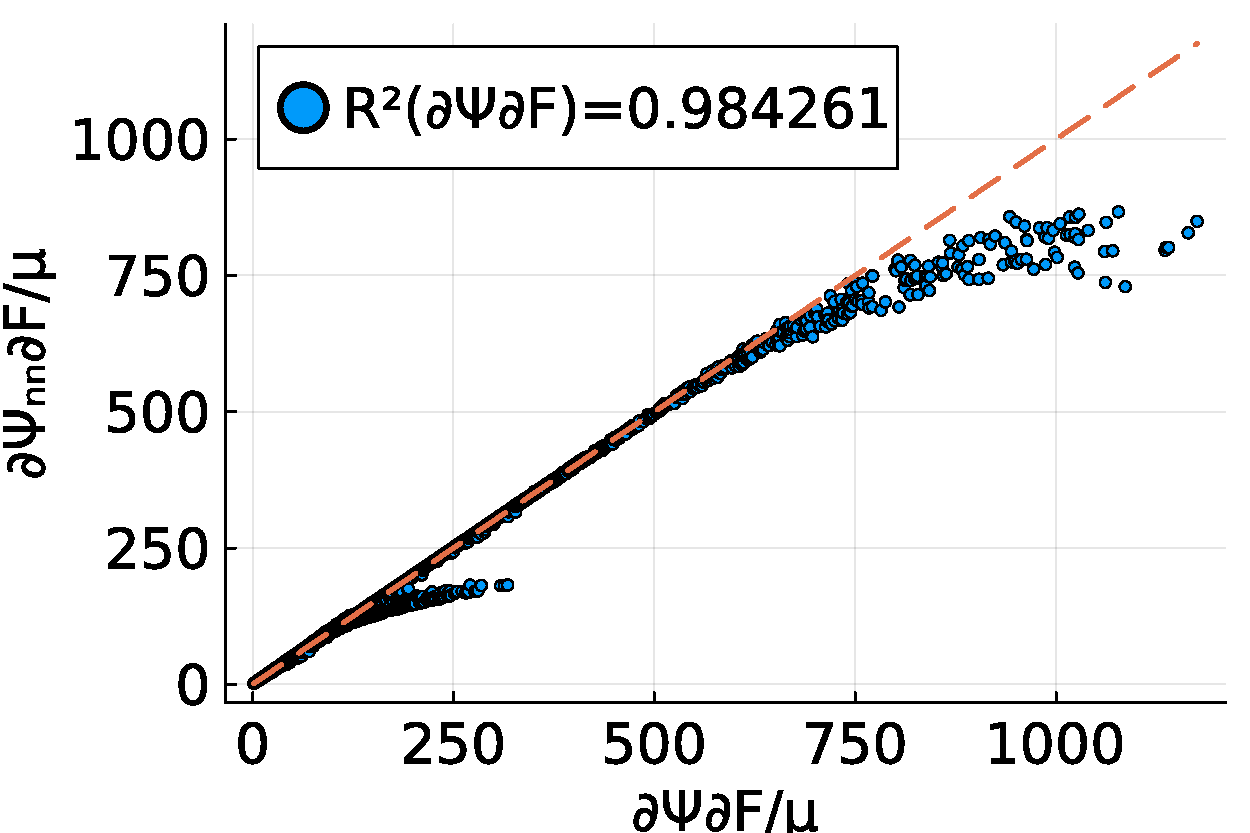
\includegraphics[width=0.3\textwidth]{Figures/ModelsStudy/_TI_ID_E0_P_CorrelationTest} &
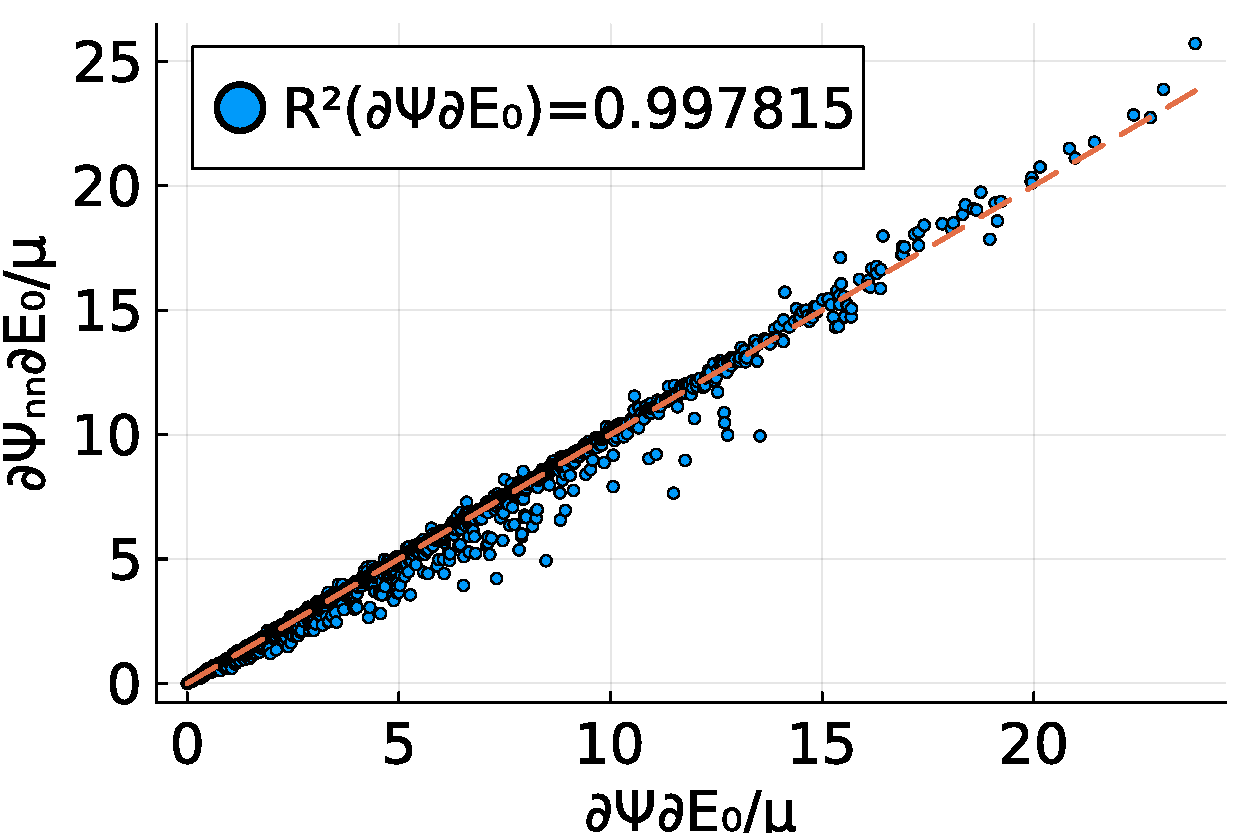
\includegraphics[width=0.3\textwidth]{Figures/ModelsStudy/_TI_ID_E0_E0_CorrelationTest} &
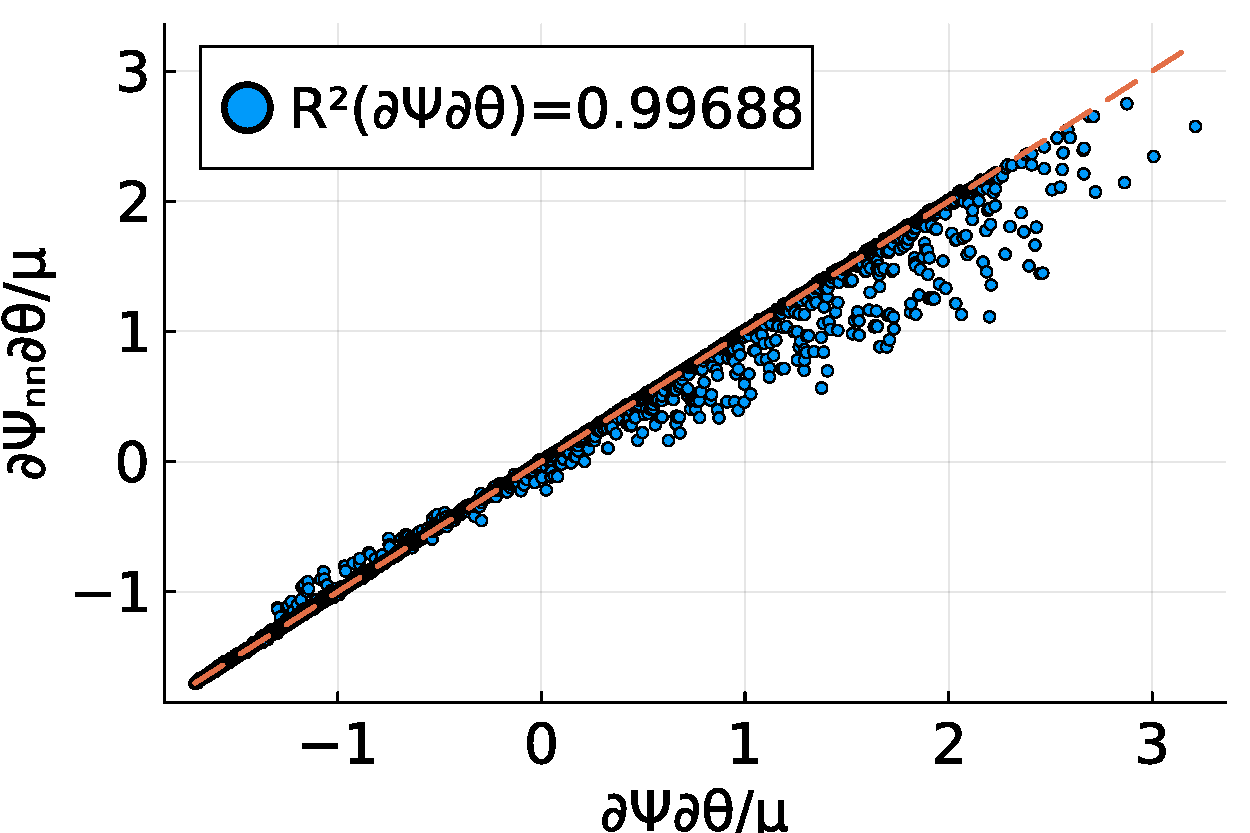
\includegraphics[width=0.3\textwidth]{Figures/ModelsStudy/_TI_ID_E0_theta_CorrelationTest} \\
%
%
	\rotatebox{90}{\,\,\,\,\,\,\,\,\,\,\textcolor{red}{\textbf{MR}}/\textcolor{blue}{\textbf{ES}}}  &	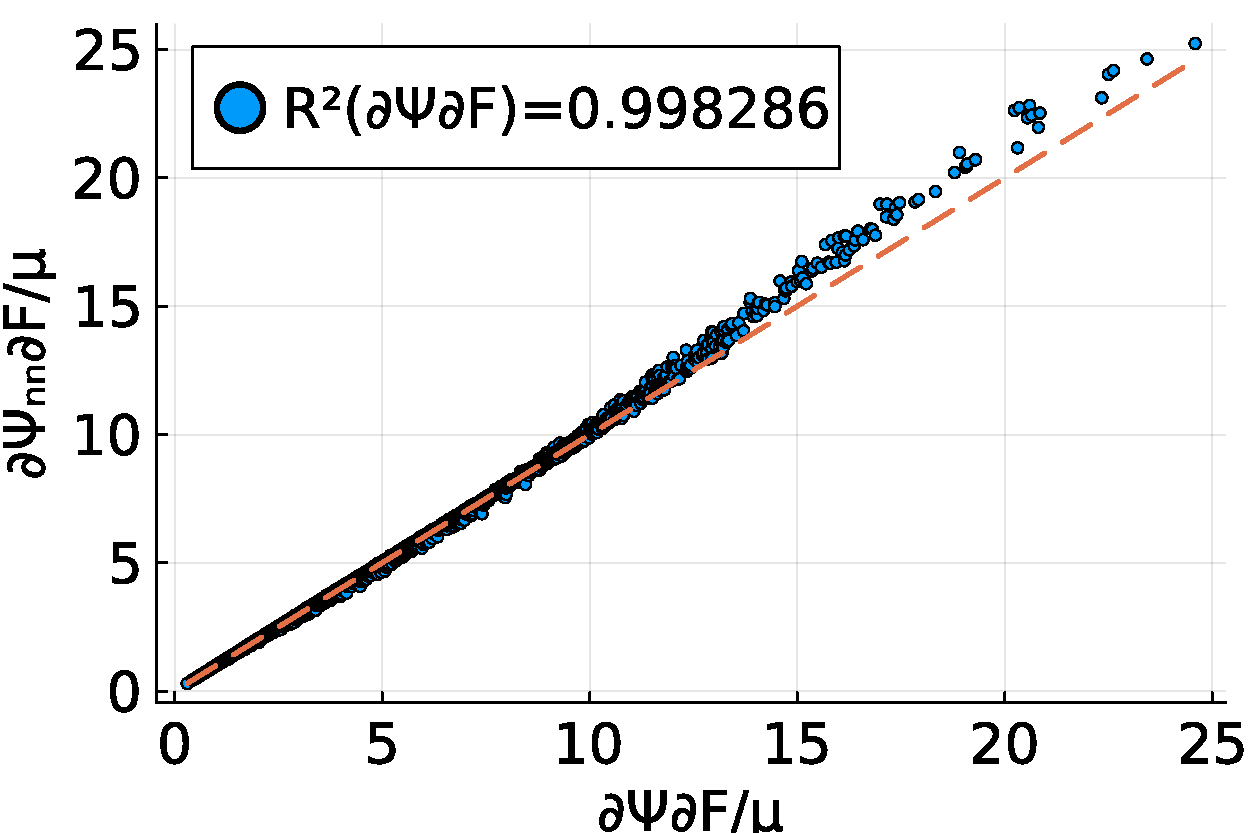
\includegraphics[width=0.3\textwidth]{Figures/ModelsStudy/_MooneyRivlin_ElectricSaturation_P_CorrelationTest} &
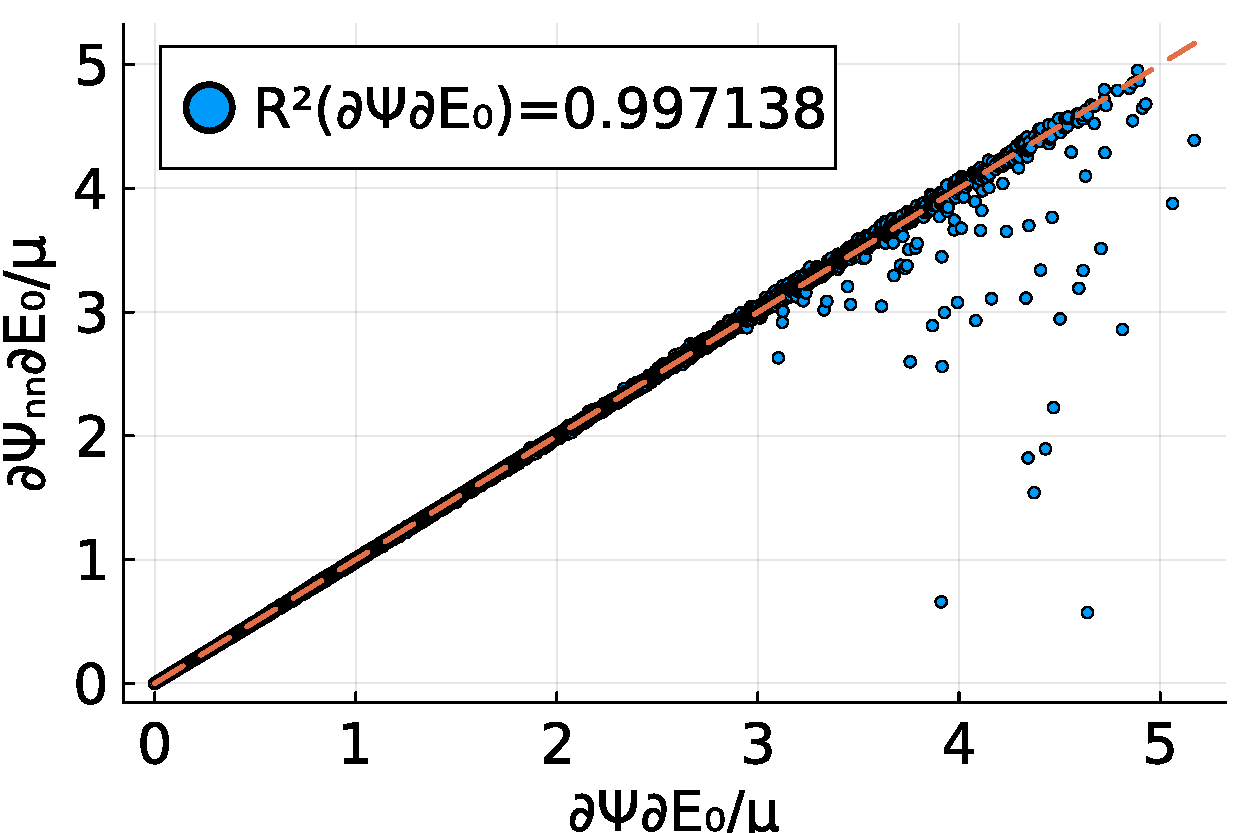
\includegraphics[width=0.3\textwidth]{Figures/ModelsStudy/_MooneyRivlin_ElectricSaturation_E0_CorrelationTest} &
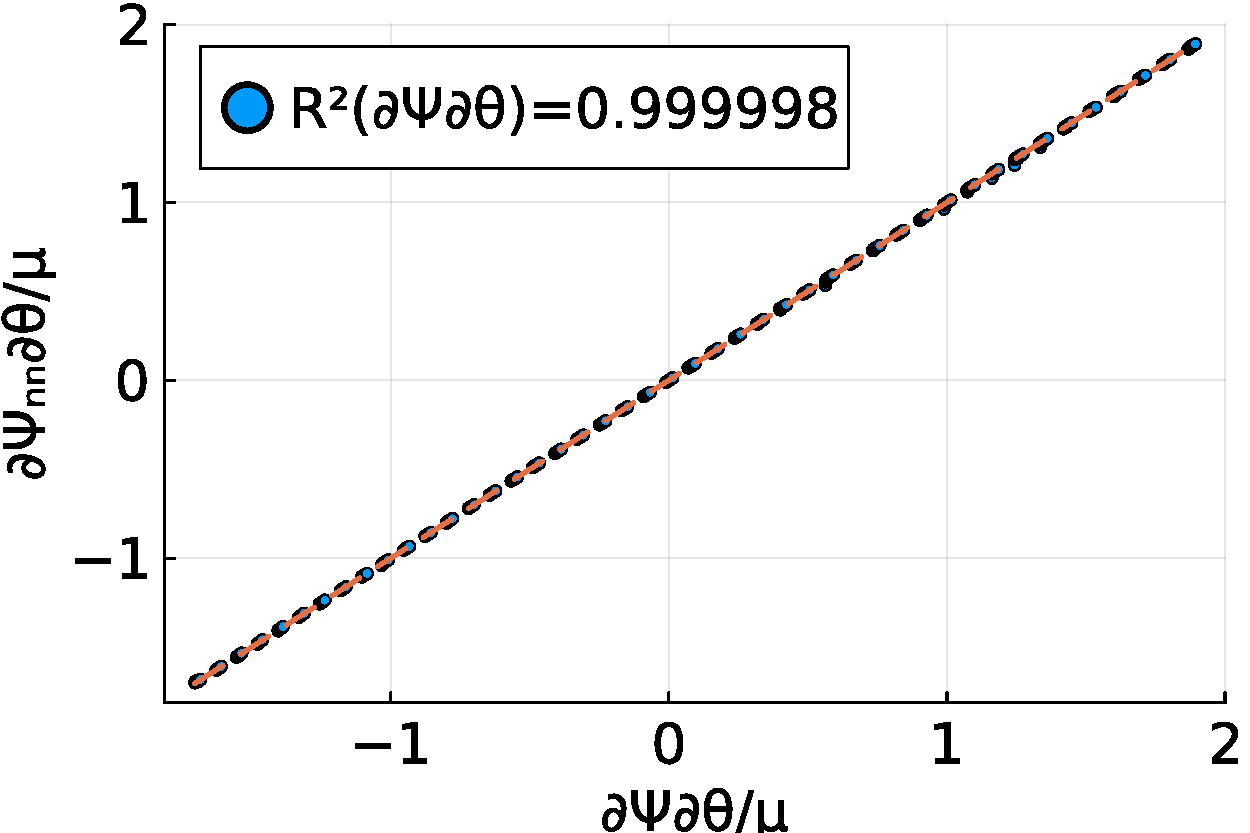
\includegraphics[width=0.3\textwidth]{Figures/ModelsStudy/_MooneyRivlin_ElectricSaturation_theta_CorrelationTest} \\
%
%
	\end{tabular}
	%
	%		\includegraphics[width=0.4\textwidth]{pictures_paper/inkscape_pictures/template_example_3.pdf}
	\caption{\textbf{Calibration Strategy 1}. Correlation of prediction $\{\partial_{\vect{F}}\Psi_{nn},\partial_{\vect{E}_0}\Psi_{nn},\partial_{\theta}\Psi_{nn}\}$ and testing data $\{\partial_{\vect{F}}\Psi,\partial_{\vect{E}_0}\Psi,\partial_{\theta}\Psi\}$ using the purely mechanical (in red) and electro-mechanical (in blue) contributions of the ground truth Helmholtz strain energy model used for the calibration. The training data represents a subset of the testing data containing the $20\%$ of the data in the latter. In all cases we have considered an architecture of $4$ layers and $8$ neurons per layer.}
	\label{fig:correlation strategy 1}
\end{figure}

















We conducted additional testing of the calibrated models in scenarios beyond those included in the training set. It is important to note that both the training and testing sets were generated using a similar in-silico data generation strategy, as outlined in Section \ref{sec:data generation strategy 1} and based on the methodology of \cite{OKunc_19_01}. Our objective is to further evaluate the calibrated potentials using a distinct data generation strategy, in which the deformation gradient tensor and the electric field are defined according to
%
\begin{equation}\label{eqn:experiments}
	\vect{F}=\begin{bmatrix}
		\lambda & \gamma & 0\\
		0&\lambda & 0\\
		0  &  0 & 1/\lambda^2
	\end{bmatrix};\,\,1\leq \lambda \leq 1.8; \qquad \vect{E}_0 =  \begin{bmatrix}
	\alpha  \\  \alpha  \\  0
\end{bmatrix}\,\,0\leq \alpha\leq 1.5\sqrt{\frac{\mu}{\varepsilon}}
\end{equation}

The objective is to assess the agreement between the derivatives of the calibrated model, $\Psi_{nn}(\vect{F}, \vect{E}0, \theta)$, and those of the ground truth model across various temperature values for the specified experimental setup. Figure \ref{fig:physical experiments} illustrates this comparison, focusing on the neural network-based potential $\Psi_{nn}(\vect{F}, \vect{E}_0, \theta)$ and a single ground truth constitutive model. The figure demonstrates a remarkable alignment between the calibrated and ground truth models, highlighting the calibrated model's capacity to accurately predict the ground truth response, even in scenarios outside its training domain.



\begin{figure}[hbtp]
	\centering
	\begin{tabular}{cc}
		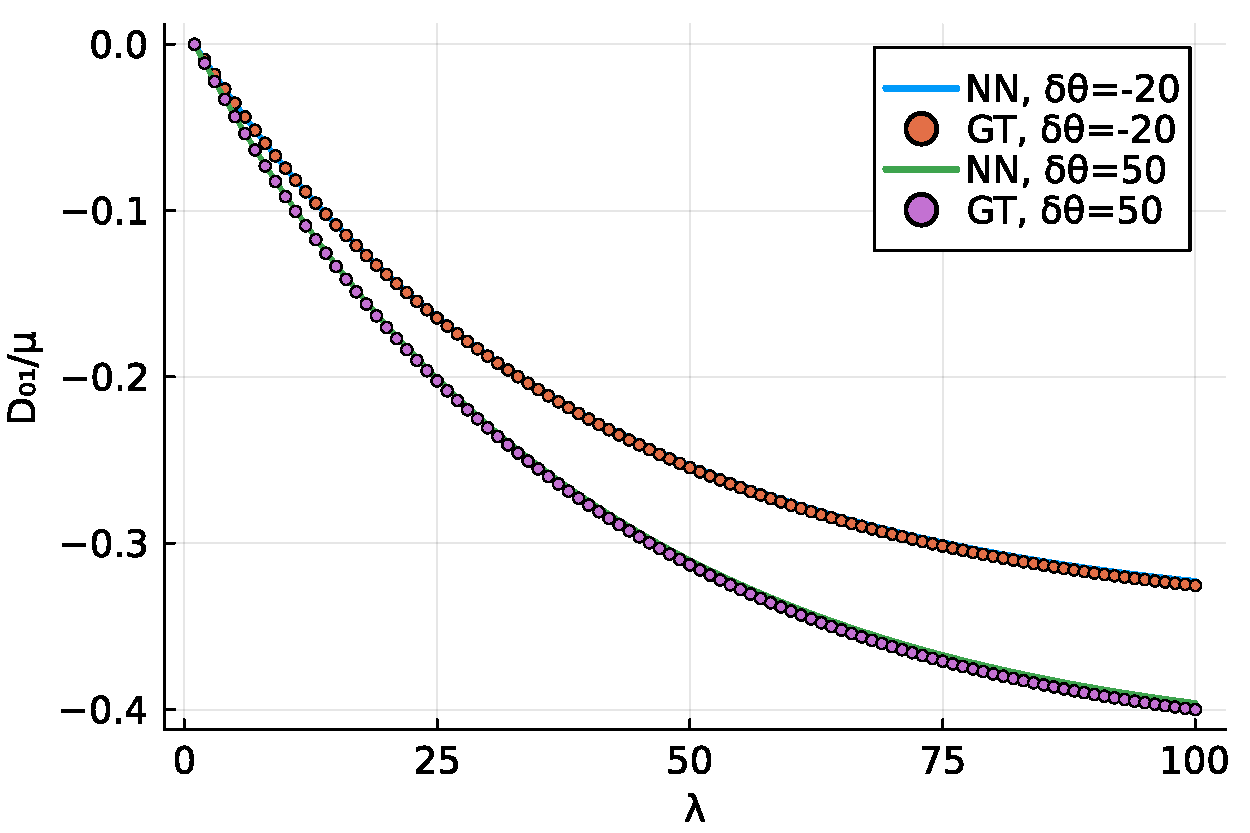
\includegraphics[width=0.4\textwidth]{Figures/PotentialStudy/_PhysicalExperiments_MooneyRivlin_ID_E0_D1} &
		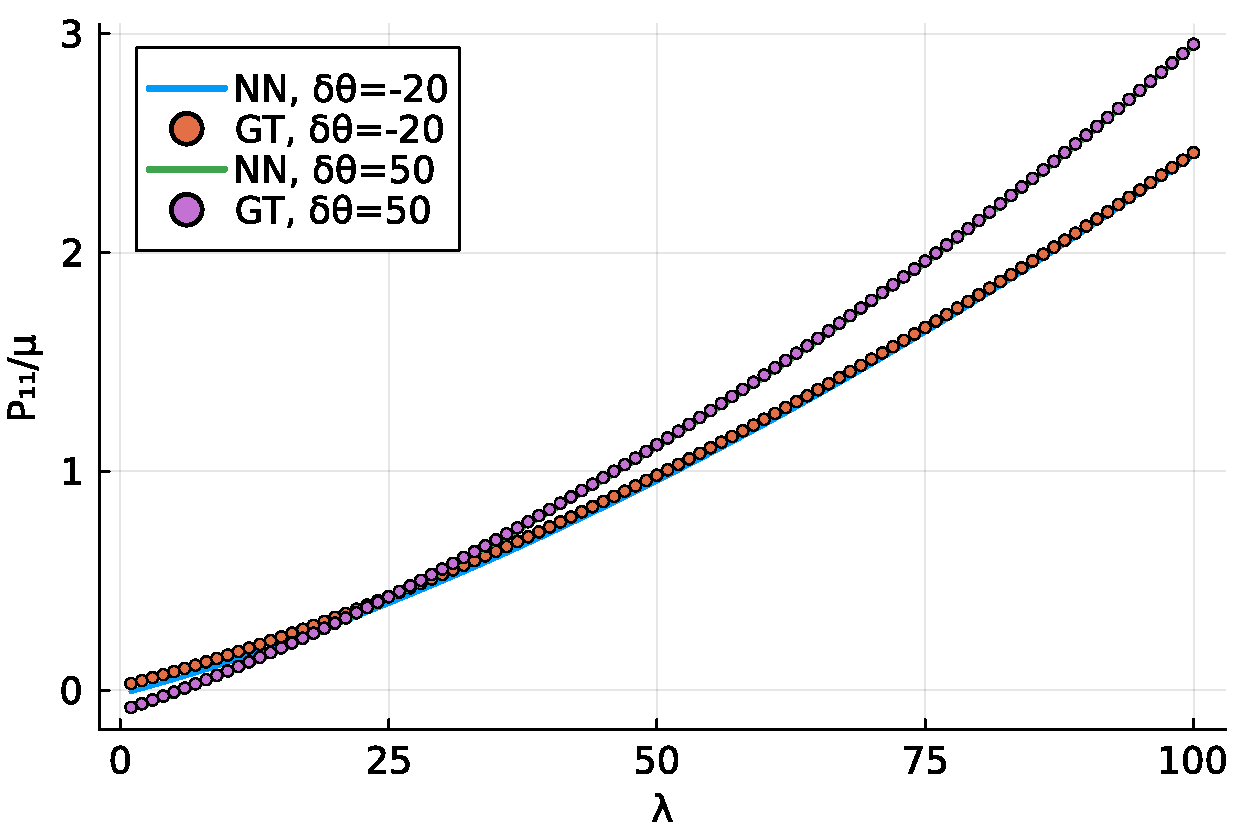
\includegraphics[width=0.4\textwidth]{Figures/PotentialStudy/_PhysicalExperiments_MooneyRivlin_ID_E0_F11}  \\
		(a)  &  (b)\\
		%
		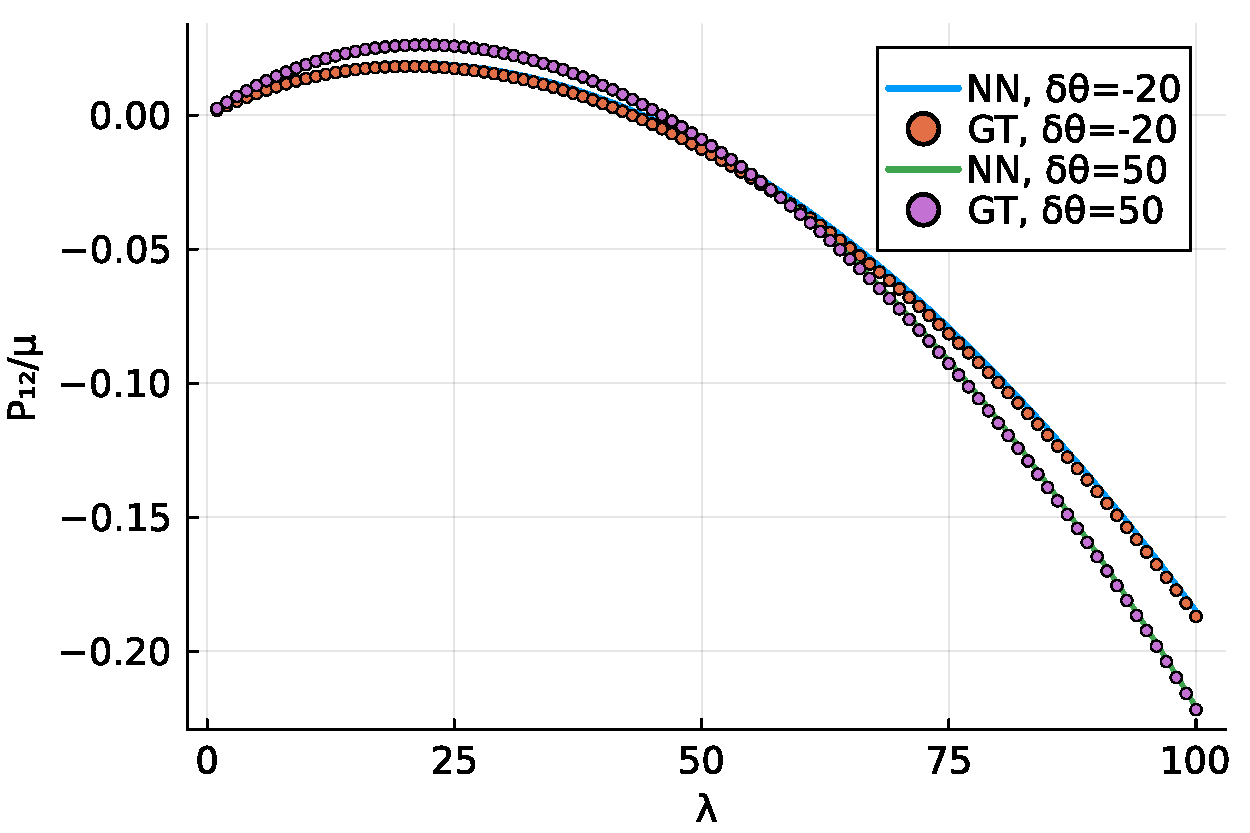
\includegraphics[width=0.4\textwidth]{Figures/PotentialStudy/_PhysicalExperiments_MooneyRivlin_ID_E0_F12} &
		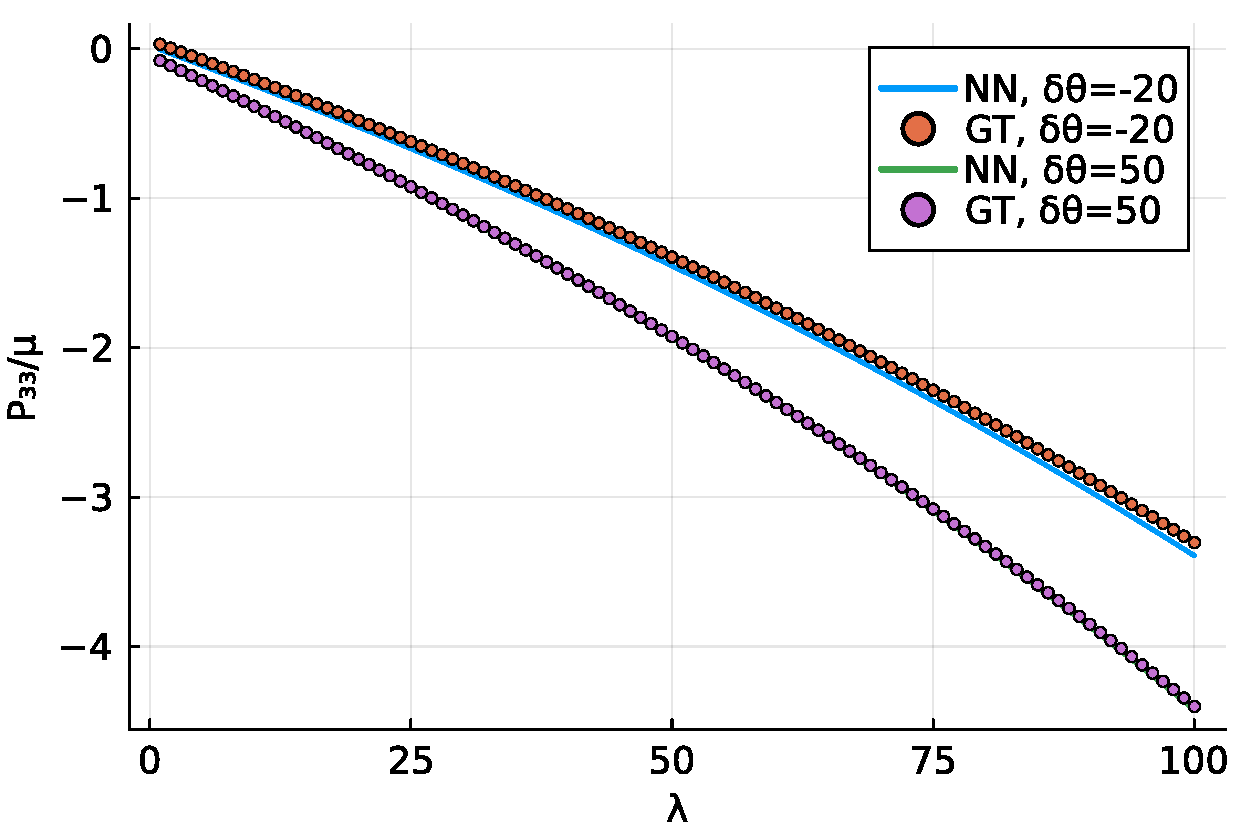
\includegraphics[width=0.4\textwidth]{Figures/PotentialStudy/_PhysicalExperiments_MooneyRivlin_ID_E0_F33}  \\
		(c)  &  (d)		
	\end{tabular}
	%
	%		\includegraphics[width=0.4\textwidth]{pictures_paper/inkscape_pictures/template_example_3.pdf}
	\caption{\textbf{Calibration Strategy 1}. Prediction of calibrated model $\Psi_{nn}(\vect{F}, \vect{E}_0, \theta)$ and ground truth model across various temperature values for the experimental setup in \eqref{eqn:experiments}. The ground truth model $\Psi(\vect{F},\vect{E}_0,\theta)$ considers a Mooney-Rivlin model for the mechanical contribution, i.e. $Psi_{m}$ and an ideal dielectric model for the electro-mechanical contribution, i.e. $\Psi_{em}$.}
	\label{fig:physical experiments}
\end{figure}


\subsubsection{Generalization results for all the thermodynamical potentials}

In the previous section, we focused exclusively on the calibration of Helmholtz-type neural network-based potentials, specifically $\Psi_{nn}(\vect{F},\vect{E}_0,\theta)$. he objective of this section, however, is to demonstrate that, while we have primarily considered a Helmholtz-type ground truth potential $\Psi(\vect{F},\vect{E}_0,\theta)$, we can successfully calibrate neural network-based potentials corresponding to alternative formulations, namely  $e_{nn}(\vect{F},\vect{D}_0,\eta)$, $\Upsilon_{nn}(\vect{F},\vect{D}_0,\theta)$ and $\Gamma_{nn}(\vect{F},\vect{E}_0,\eta)$, as outlined in Section \ref{sec:fundamentals strategy 1}. o illustrate this capability, we consider the following case:

\begin{itemize}
	\item fixed neural network architecture with 4 hidden layers and 8 neurons
	
	\item ground truth model with $\Psi_m$ corresponding with a Mooney-Rivlin model and $\Psi_{em}$ with an ideal dielectric model.
\end{itemize}

Under such scenario, Figure \ref{fig:strategy 1--the potentials} presents the correlation results for the test dataset, which is larger than the training dataset, for the four potentials, namely $\Psi_{nn}(\vect{F},\vect{E}_0,\theta)$, $e_{nn}(\vect{F},\vect{D}_0,\eta)$, $\Upsilon_{nn}(\vect{F},\vect{D}_0,\theta)$ and $\Gamma_{nn}(\vect{F},\vect{E}_0,\eta)$. The figure demonstrates an excellent agreement between the predictions made by the calibrated potentials and the ground truth model, confirming the reliability of the calibrated models in predicting the behavior of the ground truth.

\begin{figure}[hbtp]
	\centering
	\begin{tabular}{ccc}
		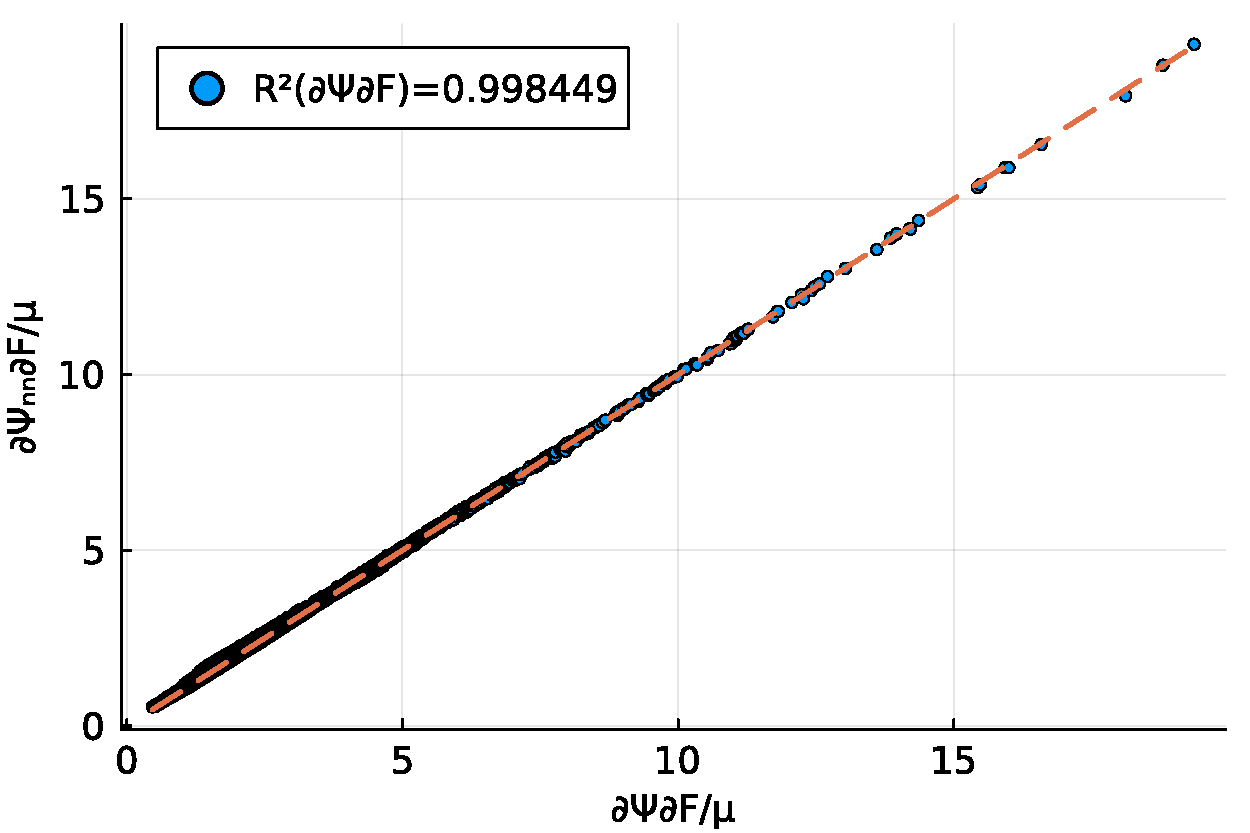
\includegraphics[width=0.33\textwidth]{Figures/PotentialStudy/Psi_P_CorrelationTest} &
		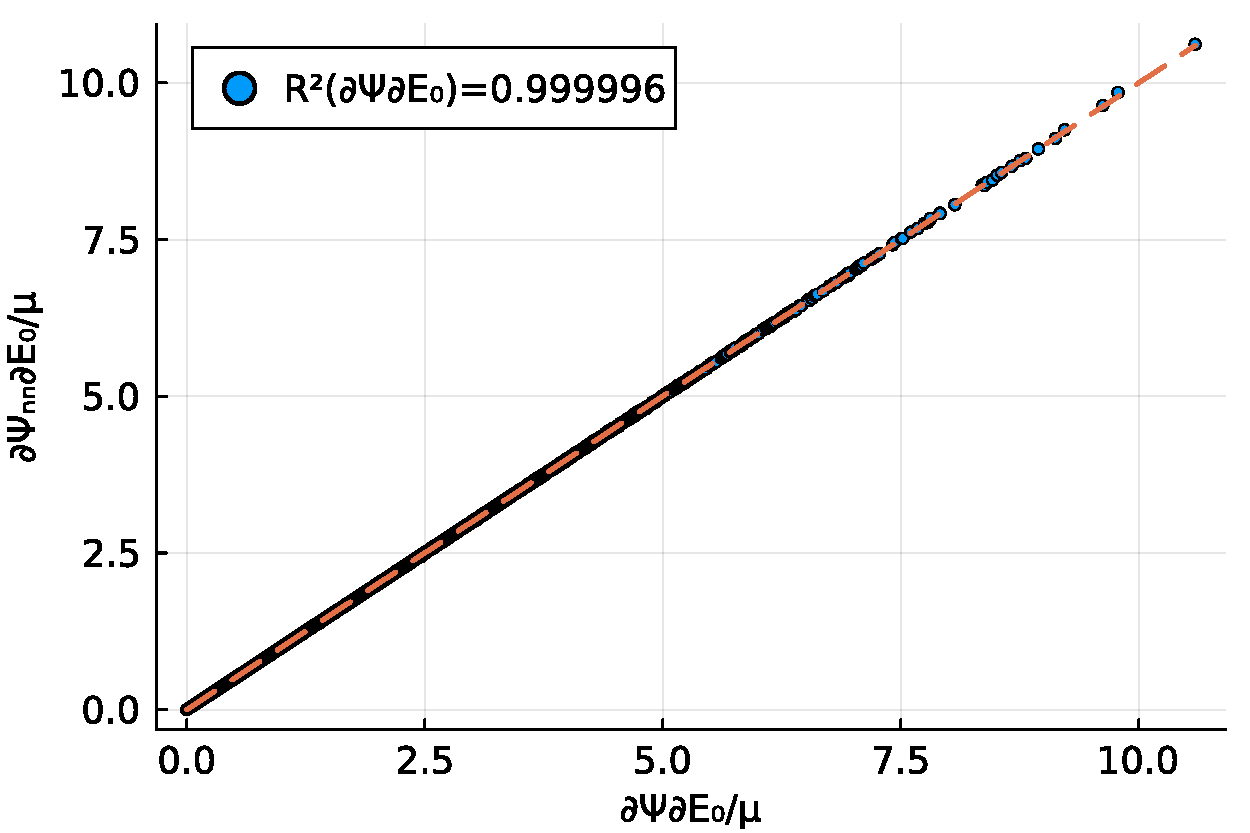
\includegraphics[width=0.33\textwidth]{Figures/PotentialStudy/Psi_E0_CorrelationTest} &
		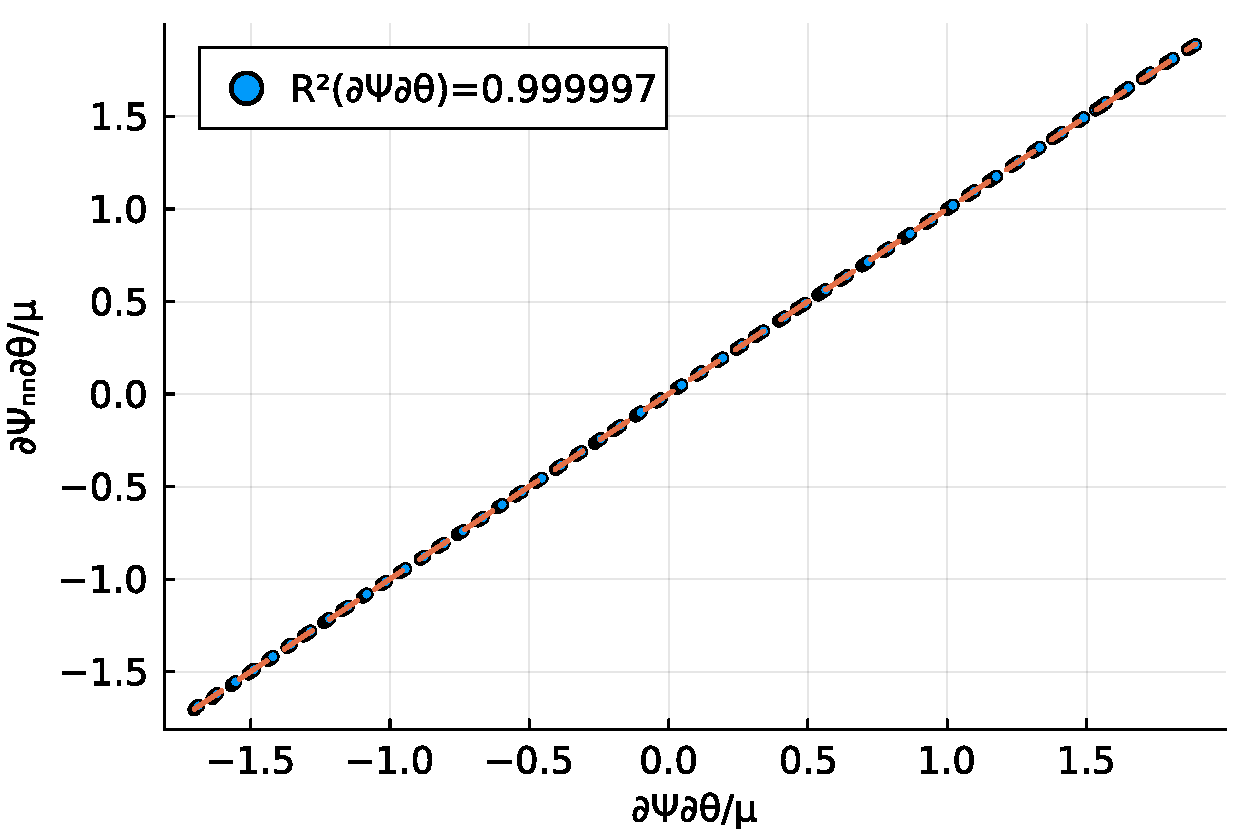
\includegraphics[width=0.33\textwidth]{Figures/PotentialStudy/Psi_theta_CorrelationTest} \\
		%
		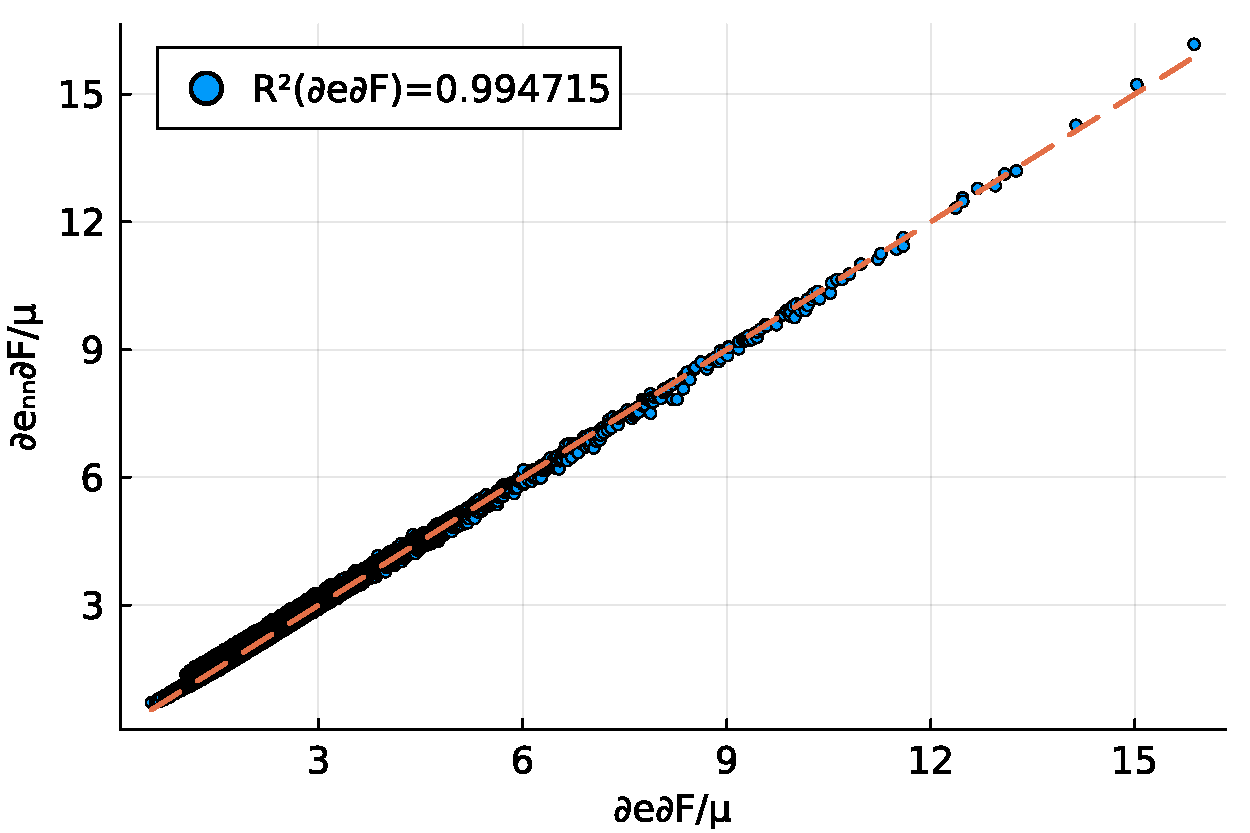
\includegraphics[width=0.33\textwidth]{Figures/PotentialStudy/e_P_CorrelationTest} &
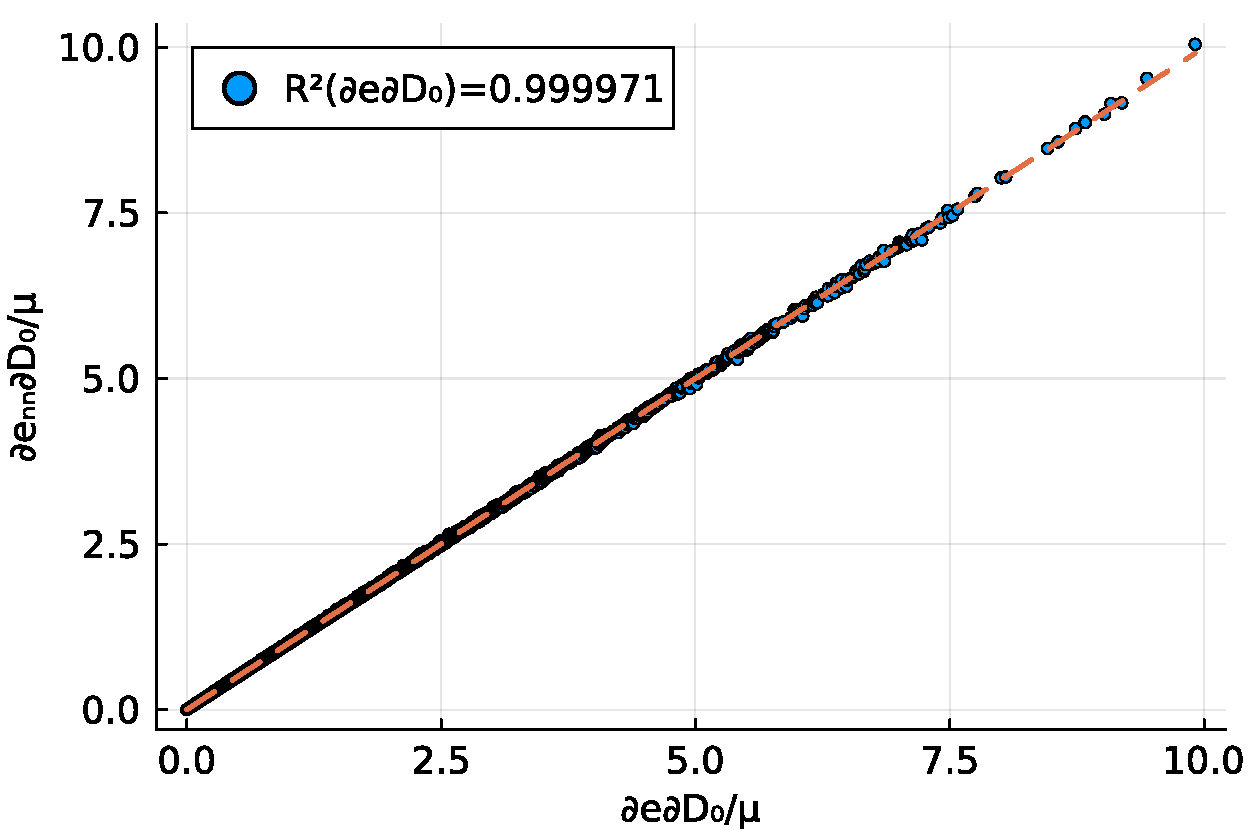
\includegraphics[width=0.33\textwidth]{Figures/PotentialStudy/e_E0_CorrelationTest} &
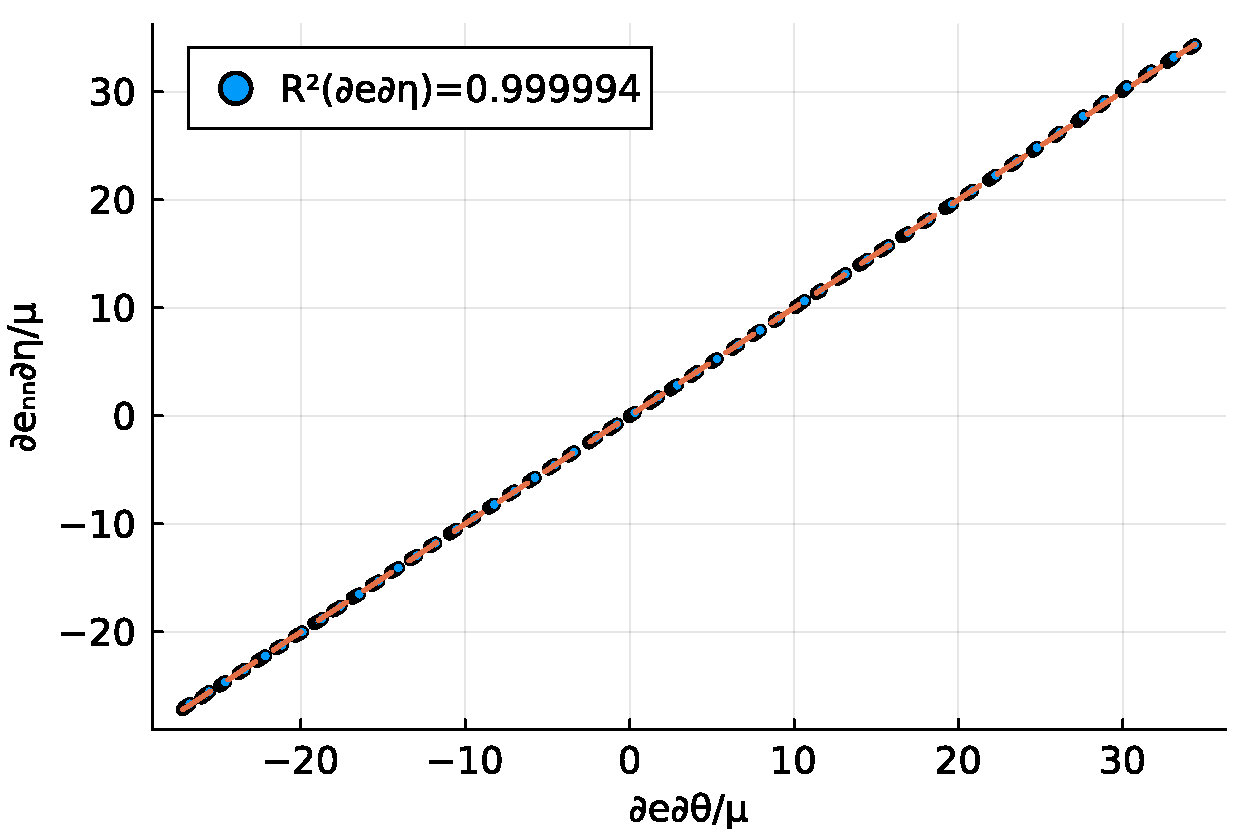
\includegraphics[width=0.33\textwidth]{Figures/PotentialStudy/e_theta_CorrelationTest} \\		%	
%	
		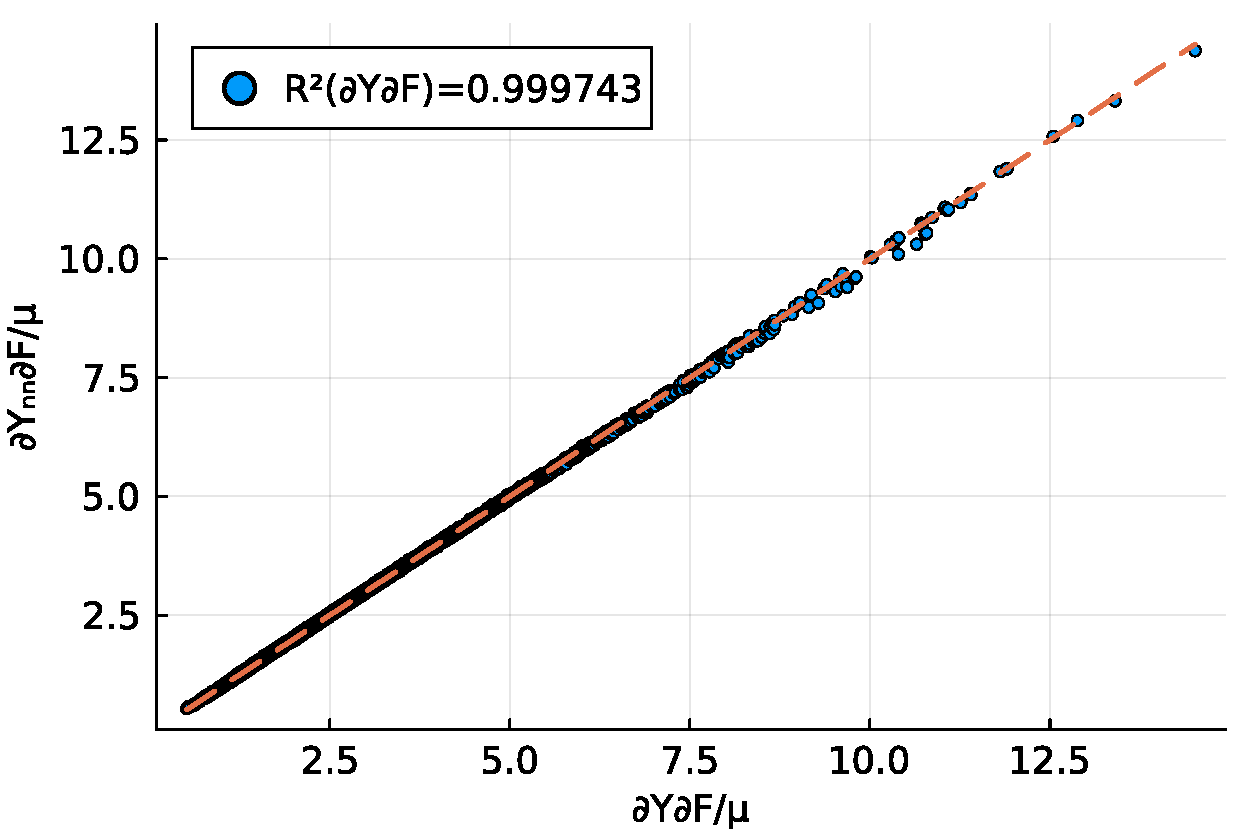
\includegraphics[width=0.33\textwidth]{Figures/PotentialStudy/Upsilon_P_CorrelationTest} &
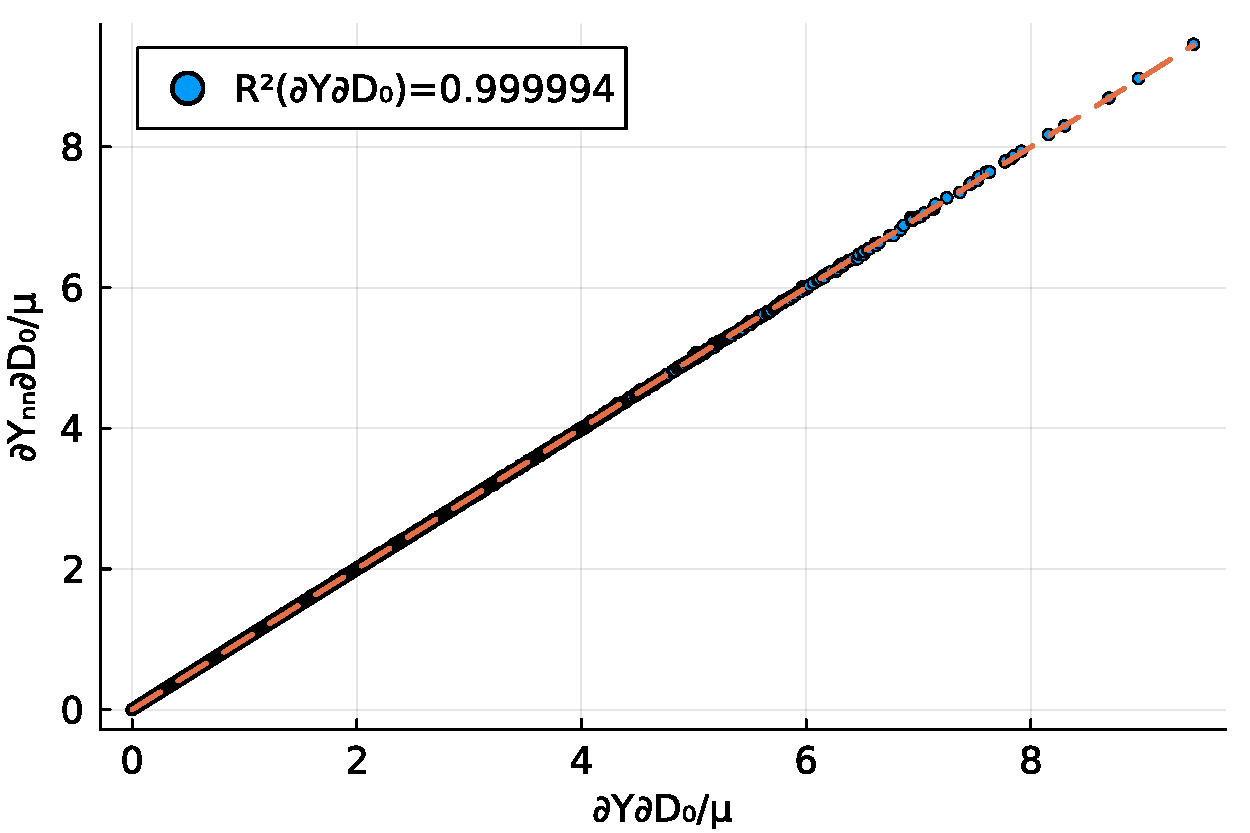
\includegraphics[width=0.33\textwidth]{Figures/PotentialStudy/Upsilon_E0_CorrelationTest} &
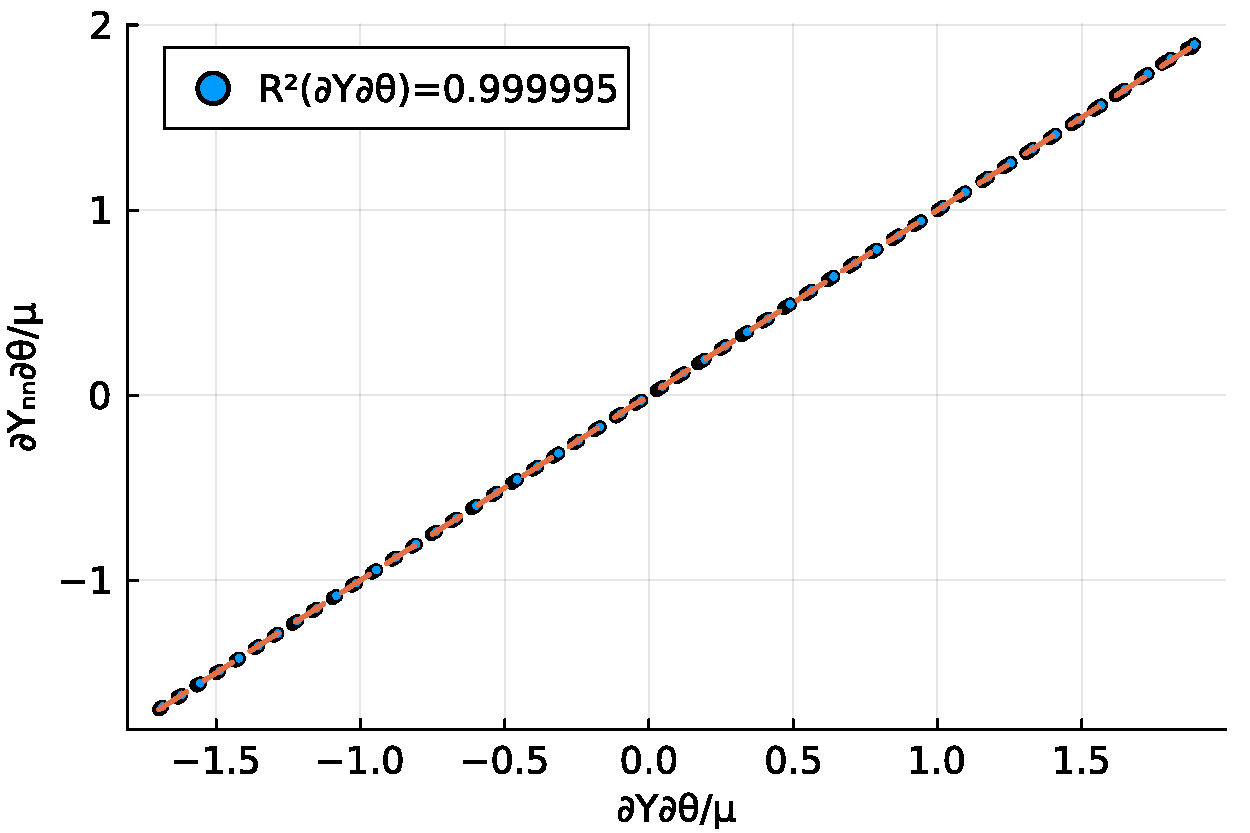
\includegraphics[width=0.33\textwidth]{Figures/PotentialStudy/Upsilon_theta_CorrelationTest} \\		%	
		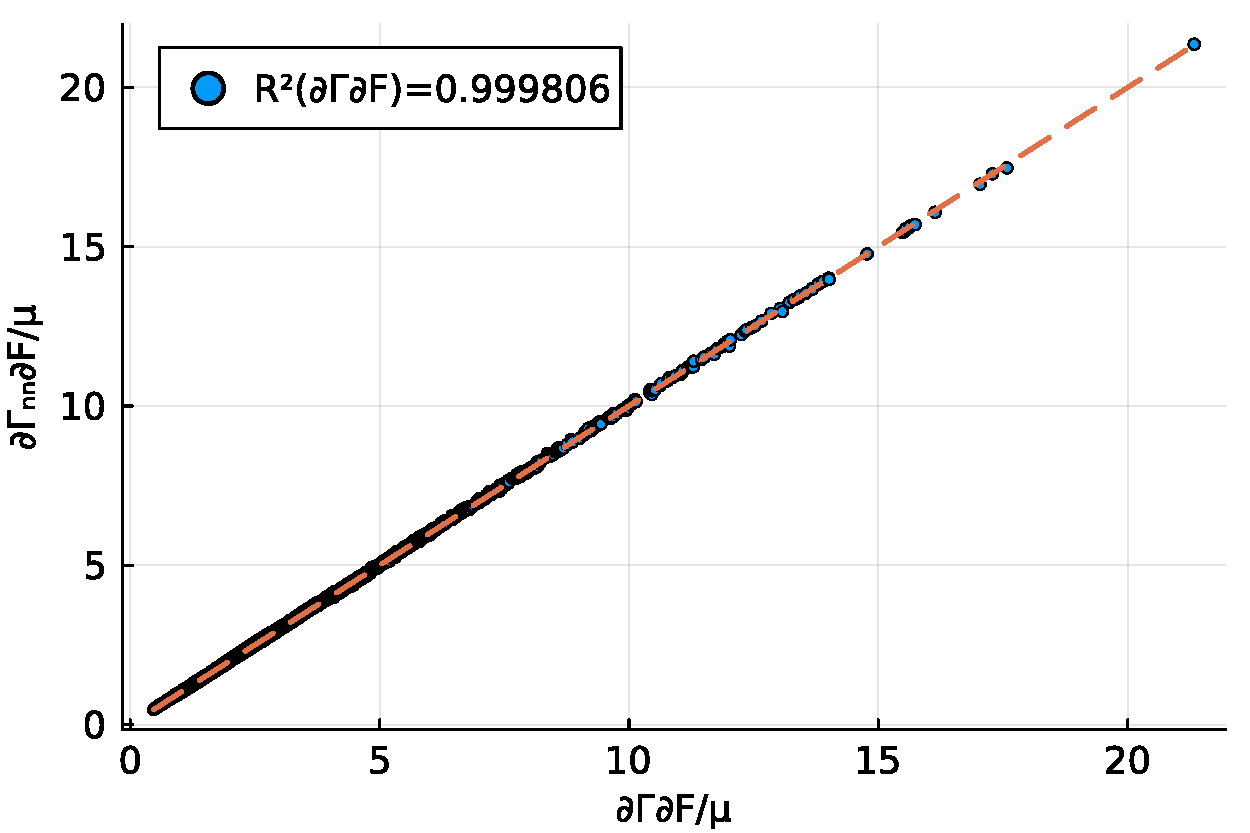
\includegraphics[width=0.33\textwidth]{Figures/PotentialStudy/Gamma_P_CorrelationTest} &
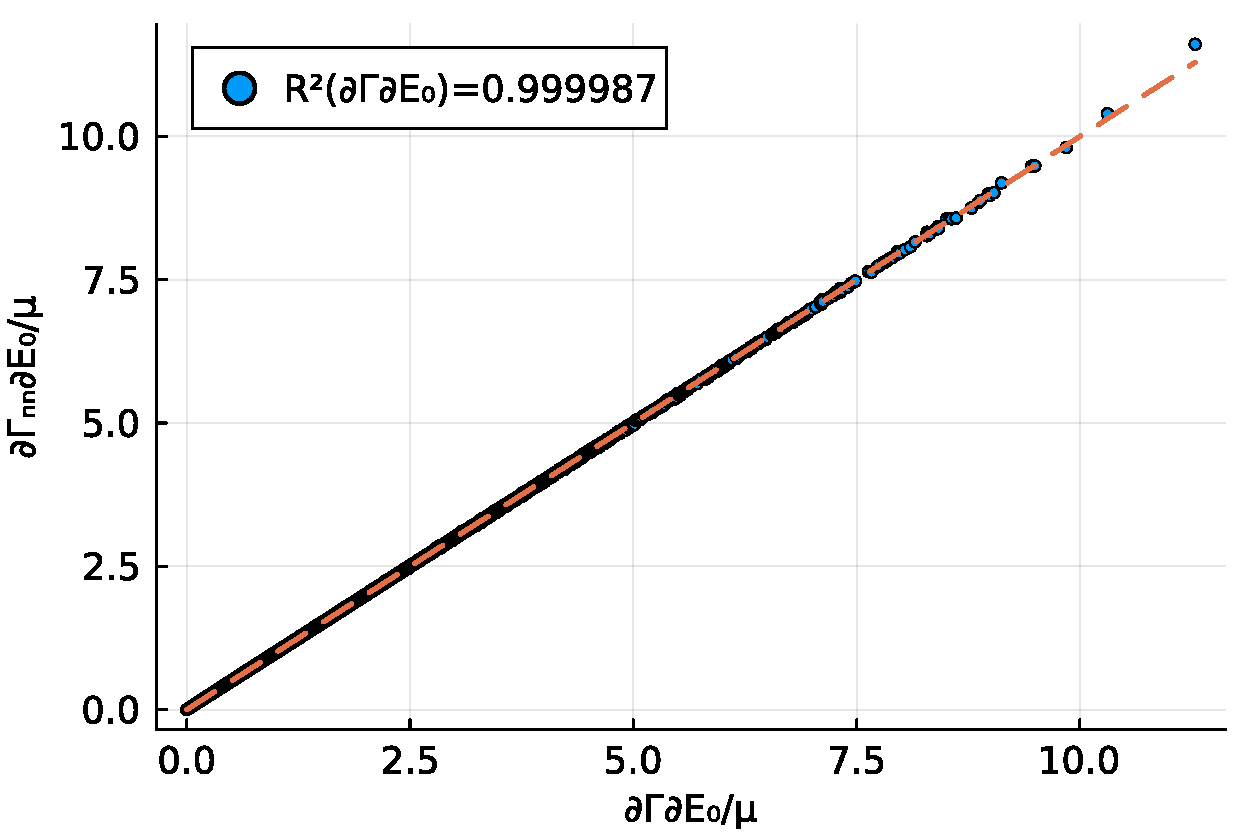
\includegraphics[width=0.33\textwidth]{Figures/PotentialStudy/Gamma_E0_CorrelationTest} &
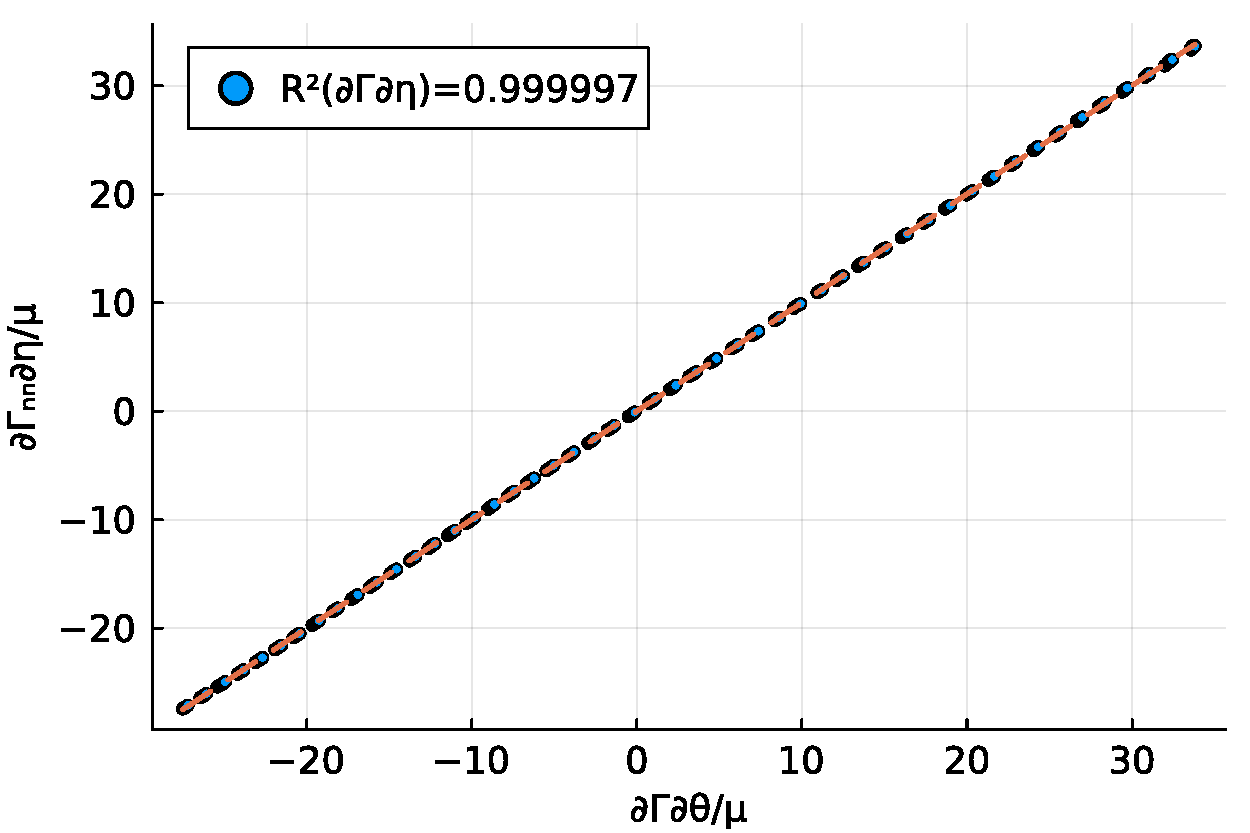
\includegraphics[width=0.33\textwidth]{Figures/PotentialStudy/Gamma_theta_CorrelationTest} \\		

	\end{tabular}
	%
	%		\includegraphics[width=0.4\textwidth]{pictures_paper/inkscape_pictures/template_example_3.pdf}
	\caption{\textbf{Calibration Strategy 1}. Correlation of prediction , $\{\partial_{\vect{F}}\Psi_{nn},\partial_{\vect{E}_0}\Psi_{nn},\partial_{\theta}\Psi_{nn}\}$, $\{\partial_{\vect{F}}e_{nn},\partial_{\vect{D}_0}d_{nn},\partial_{\eta}e_{nn}\}$, $\{\partial_{\vect{F}}\Upsilon_{nn},\partial_{\vect{D}_0}\Upsilon_{nn},\partial_{\theta}\Upsilon_{nn}\}$ and $\{\partial_{\vect{F}}\Gamma_{nn},\partial_{\vect{E}_0}\Gamma_{nn},\partial_{\eta}\Gamma_{nn}\}$ and their testing data counterparts. In all cases we have considered an architecture of $4$ layers and $8$ neurons per layer.}
	\label{fig:strategy 1--the potentials}
\end{figure}

\clearpage


\subsubsection{Polyconvex calibration}\label{sec:polyconvexity}

STUDY OF POLYCONVEXITY FOR POTENTIAL e

\begin{figure}[hbtp]
	\centering
	\begin{tabular}{ccc}
		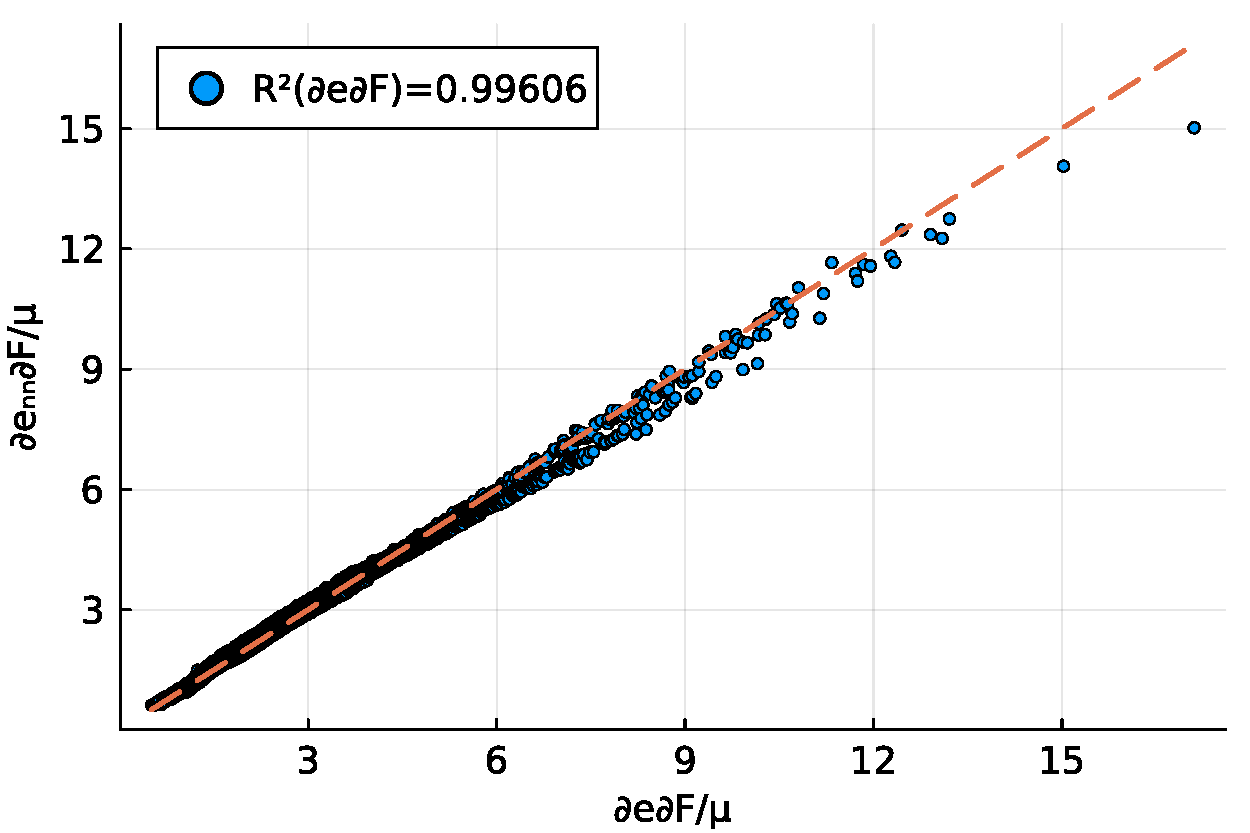
\includegraphics[width=0.33\textwidth]{Figures/PotentialStudy/e_pol_P_CorrelationTest} &
		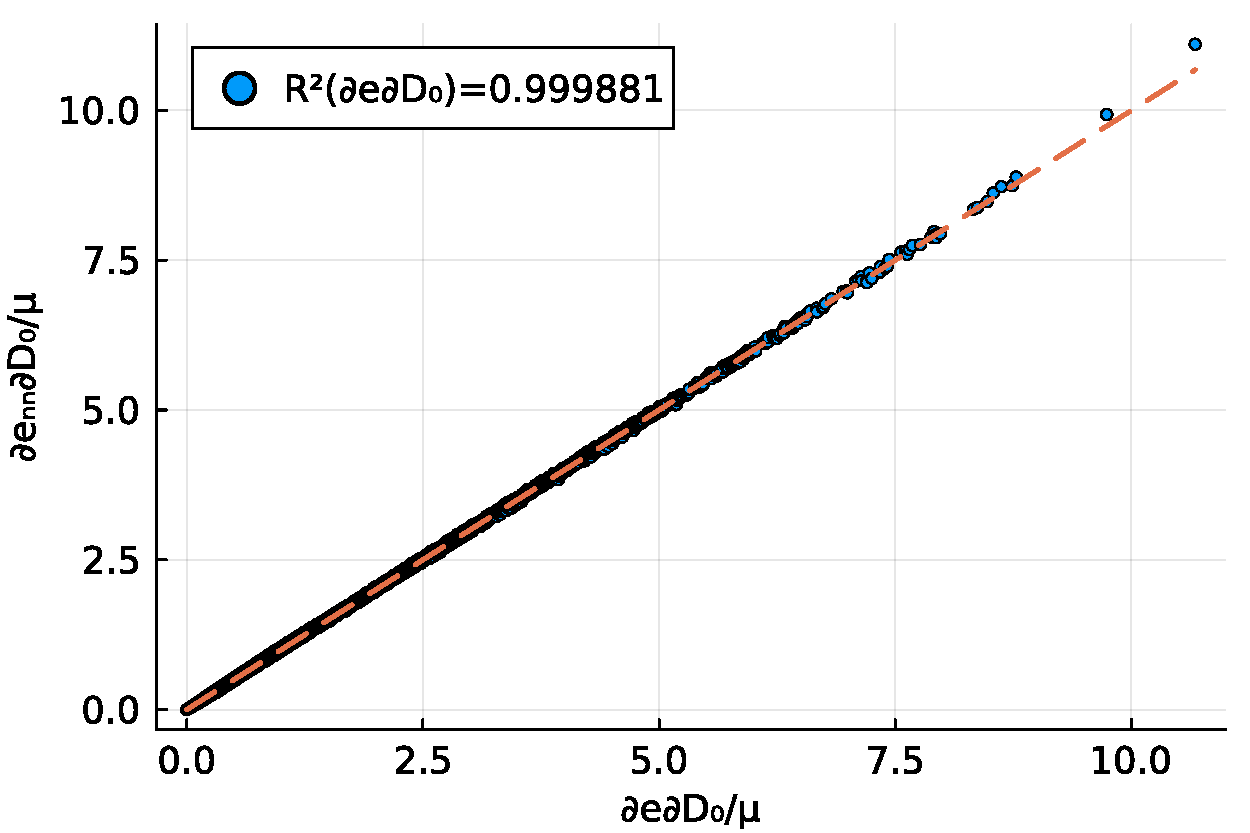
\includegraphics[width=0.33\textwidth]{Figures/PotentialStudy/e_pol_E0_CorrelationTest} &
		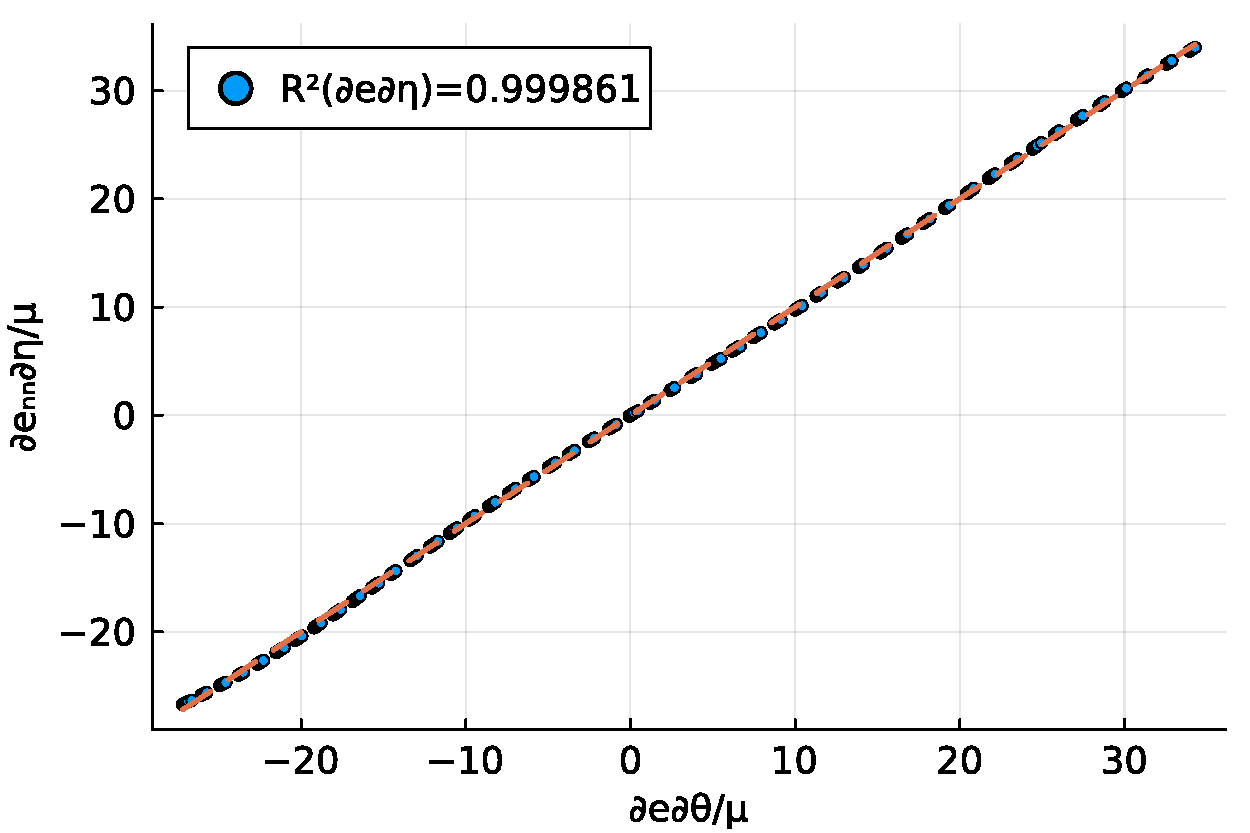
\includegraphics[width=0.33\textwidth]{Figures/PotentialStudy/e_pol_theta_CorrelationTest} \\

	\end{tabular}
	%
	%		\includegraphics[width=0.4\textwidth]{pictures_paper/inkscape_pictures/template_example_3.pdf}
	\caption{\textbf{Calibration Strategy 1}.}
	\label{fig:example 1 energy balance}
\end{figure}


\subsubsection{Generalization to unseen experiments}





\clearpage


\subsection{Calibration strategy 2: $\theta$-based potentials}


\subsubsection{Neural network architecture's influence: $\Psi_{nn}$ neural network-based ground truth models}


\begin{table}[hbtp!]
	\centering
	\begin{tabular}{c c c c c c c c c c c c}
		\toprule
		\rowcolor{gray!30}	\small{} & $n_L+1$ & 1 &  2& 3& 4& 5& 1& 2& 3& 4 & 5\\
		\midrule 
		\rowcolor{gray!30}	\small{} & $n_n$ & 8 & 8& 8& 8 &8 &16& 16& 16& 16 &  16\\
		\midrule
		\multirow{3}{*}{\rotatebox{90}{\textcolor{red}{\textbf{MR}}/\textcolor{blue}{\textbf{ID}}}}  &$R^2(\partial_{\vect{F}}\Psi)$ & 1 & 1& 1 & 1 & 1& 1& 1& 1& 1 & 1\\
		&$R^2(\partial_{\vect{F}}\Psi)$ & 1 & 1& 1 & 1 & 1& 1& 1& 1& 1 & 1\\
		&$R^2(\partial_{\vect{F}}\Psi)$ & 1 & 1& 1 & 1 & 1& 1& 1& 1& 1 & 1\\	
		\midrule
		\multirow{3}{*}{\rotatebox{90}{QMR/ID}} &$R^2(\partial_{\vect{F}}\Psi)$ & 1 & 1& 1 & 1 & 1& 1& 1& 1& 1 &  1\\
		&$R^2(\partial_{\vect{F}}\Psi)$ & 1 & 1& 1 & 1 & 1& 1& 1& 1& 1 &  1\\
		&$R^2(\partial_{\vect{F}}\Psi)$ & 1 & 1& 1 & 1 & 1& 1& 1& 1& 1 & 1\\	
		\midrule
		\multirow{3}{*}{\rotatebox{90}{Y/ID}} &$R^2(\partial_{\vect{F}}\Psi)$ & 1 & 1& 1 & 1 & 1& 1& 1& 1& 1 &  1\\
		&$R^2(\partial_{\vect{F}}\Psi)$ & 1 & 1& 1 & 1 & 1& 1& 1& 1& 1 &  1\\
		&$R^2(\partial_{\vect{F}}\Psi)$ & 1 & 1& 1 & 1 & 1& 1& 1& 1& 1 & 1\\	
		\midrule
		\multirow{3}{*}{\rotatebox{90}{G/ID}} &$R^2(\partial_{\vect{F}}\Psi)$ & 1 & 1& 1 & 1 & 1& 1& 1& 1& 1 &  1\\
		&$R^2(\partial_{\vect{F}}\Psi)$ & 1 & 1& 1 & 1 & 1& 1& 1& 1& 1 &  1\\
		&$R^2(\partial_{\vect{F}}\Psi)$ & 1 & 1& 1 & 1 & 1& 1& 1& 1& 1 & 1\\	
		\midrule
		\multirow{3}{*}{\rotatebox{90}{TI/ID}} &$R^2(\partial_{\vect{F}}\Psi)$ & 1 & 1& 1 & 1 & 1& 1& 1& 1& 1 &  1\\
		&$R^2(\partial_{\vect{F}}\Psi)$ & 1 & 1& 1 & 1 & 1& 1& 1& 1& 1 &  1\\
		&$R^2(\partial_{\vect{F}}\Psi)$ & 1 & 1& 1 & 1 & 1& 1& 1& 1& 1 & 1\\	
		\midrule
		\multirow{3}{*}{\rotatebox{90}{MR/ES}} &$R^2(\partial_{\vect{F}}\Psi)$ & 1 & 1& 1 & 1 & 1& 1& 1& 1& 1 &  1\\
		&$R^2(\partial_{\vect{F}}\Psi)$ & 1 & 1& 1 & 1 & 1& 1& 1& 1& 1 &  1\\
		&$R^2(\partial_{\vect{F}}\Psi)$ & 1 & 1& 1 & 1 & 1& 1& 1& 1& 1 & 1\\	
		\midrule
	\end{tabular}
	\caption{}
	\label{table: results calibration strategy 1}
\end{table}


\clearpage



\begin{figure}[hbtp!]
	\centering
	\begin{tabular}{cccc}
		\rotatebox{90}{\,\,\,\,\,\,\,\,\,\,\textcolor{red}{\textbf{MR}}/\textcolor{blue}{\textbf{ID}}}  &		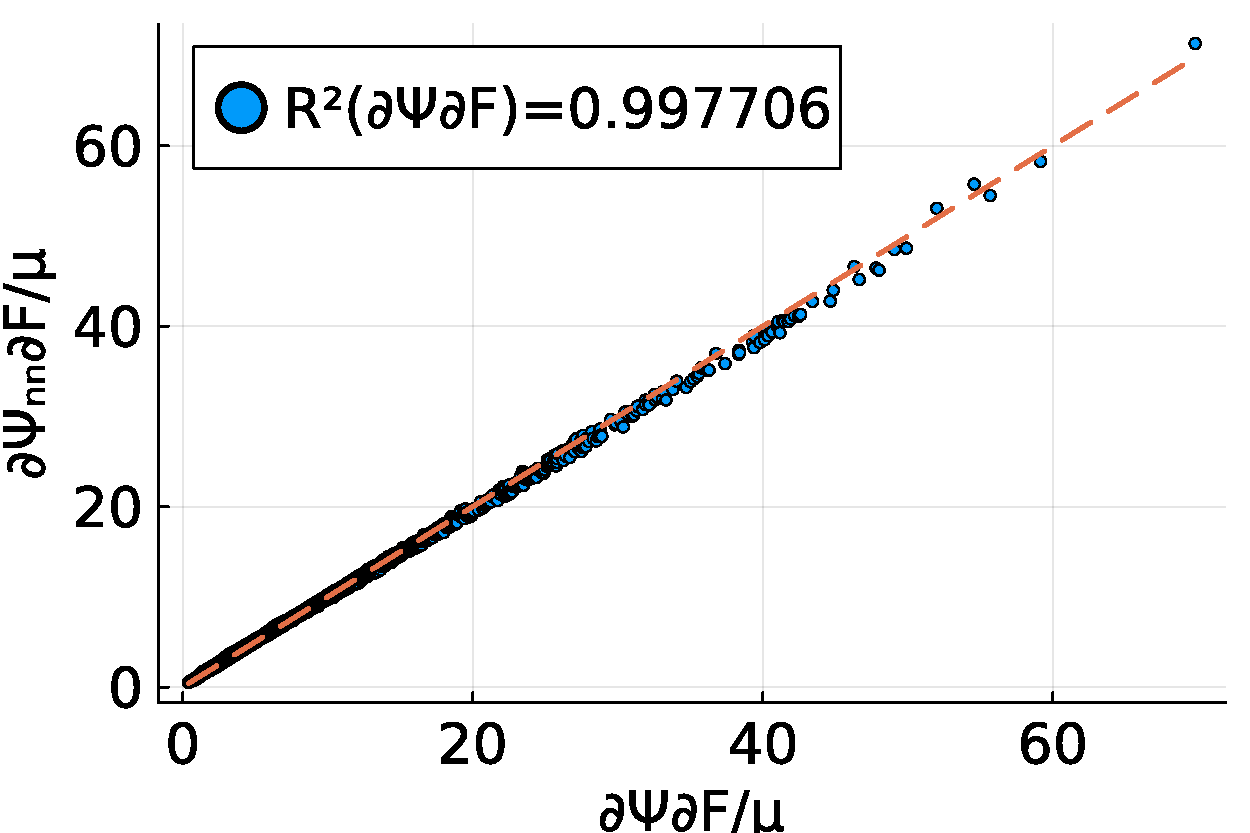
\includegraphics[width=0.33\textwidth]{Figures/ModelsStudy/_MooneyRivlin_ID_E0_P_CorrelationTest} &
		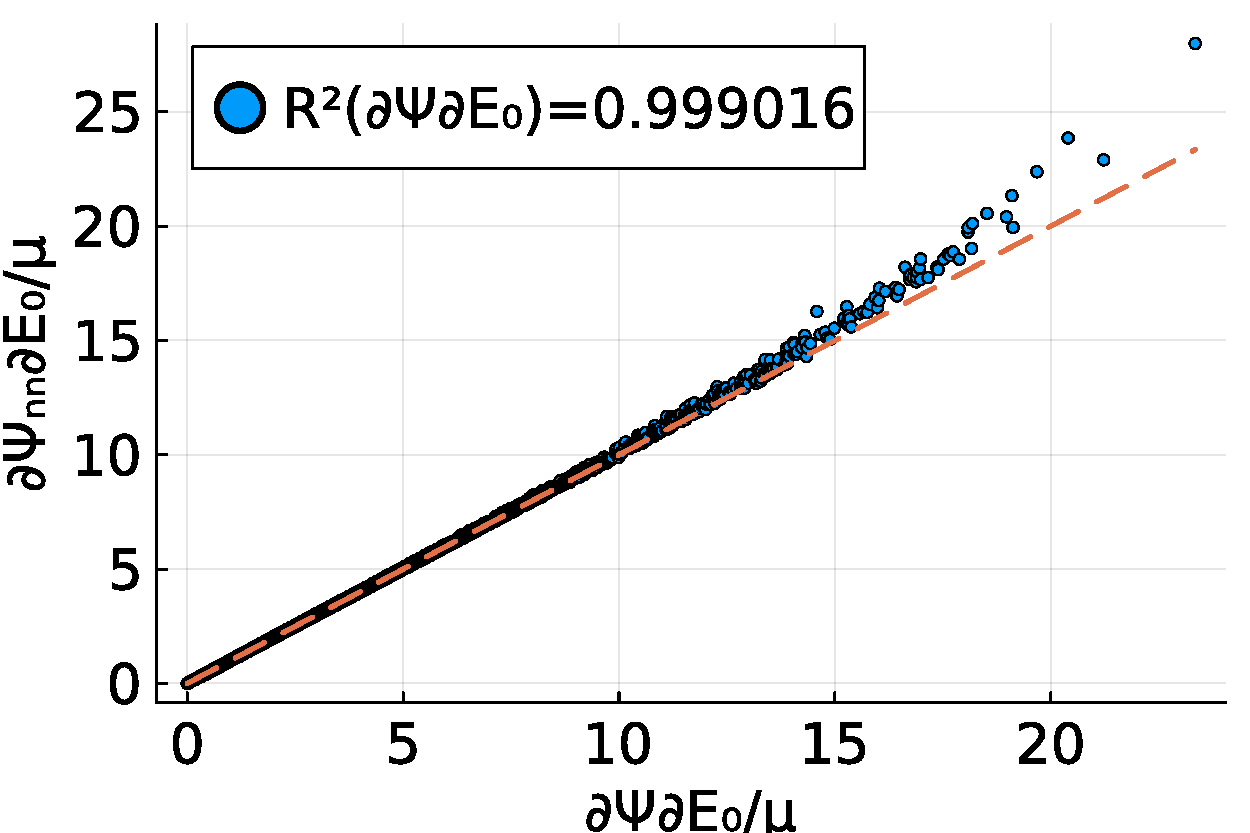
\includegraphics[width=0.33\textwidth]{Figures/ModelsStudy/_MooneyRivlin_ID_E0_E0_CorrelationTest} &
		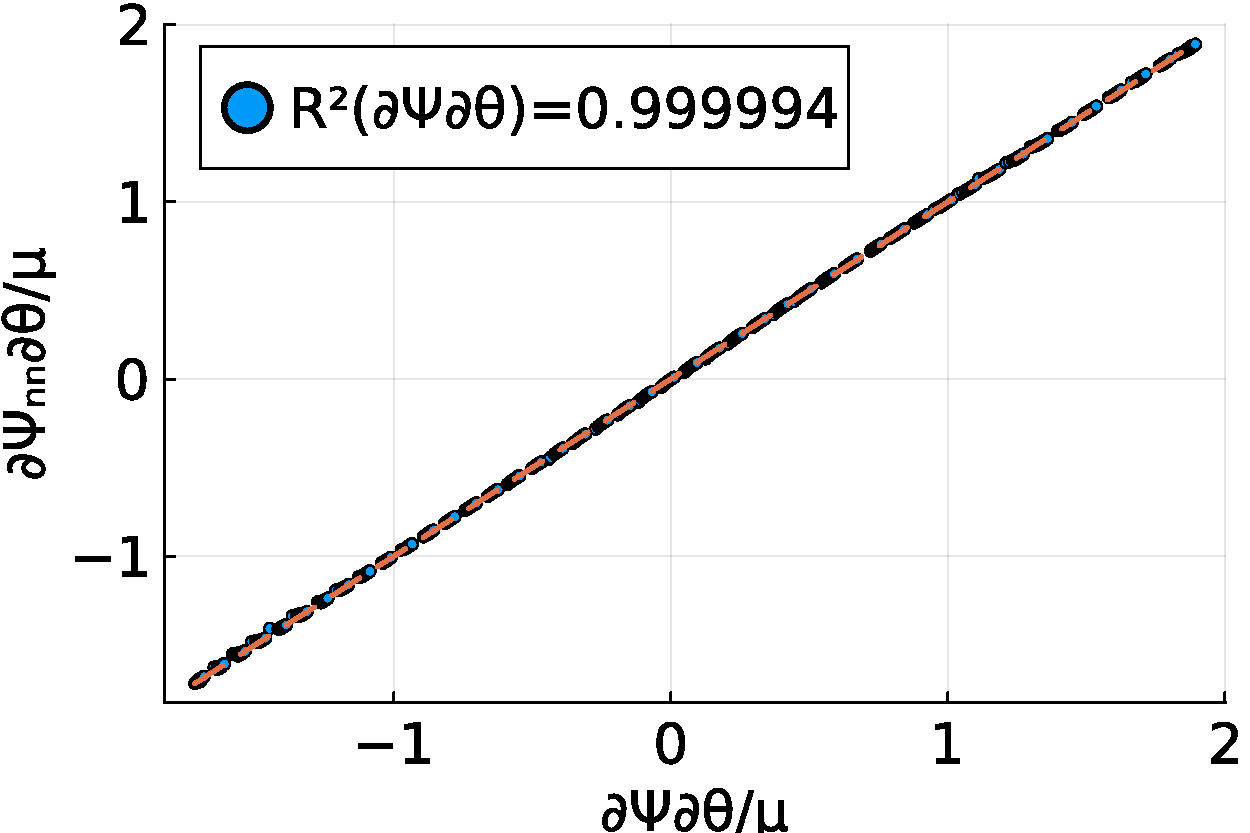
\includegraphics[width=0.33\textwidth]{Figures/ModelsStudy/_MooneyRivlin_ID_E0_theta_CorrelationTest} \\
		%
		\rotatebox{90}{\,\,\,\,\,\,\,\,\,\,\textcolor{red}{\textbf{QMR}}/\textcolor{blue}{\textbf{ID}}} &	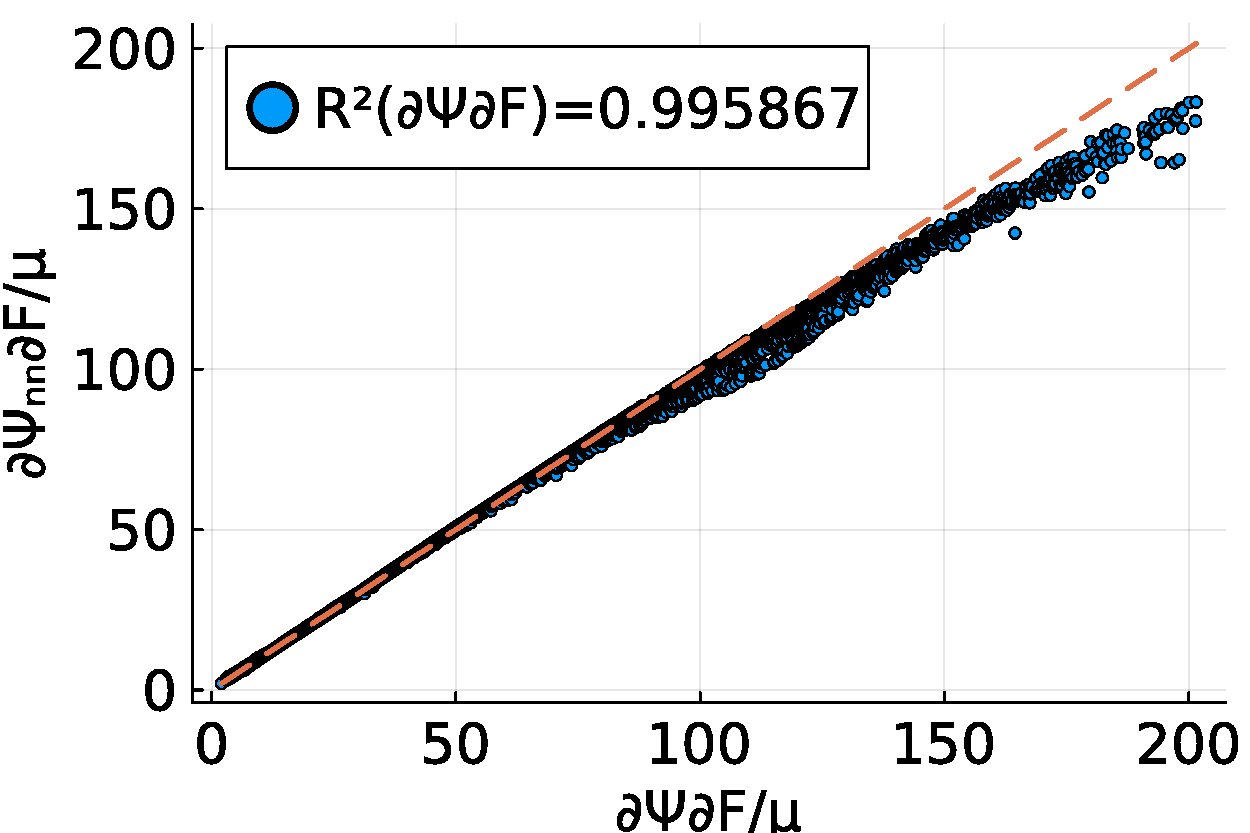
\includegraphics[width=0.33\textwidth]{Figures/ModelsStudy/_QuadraticMooneyRivlin_ID_E0_P_CorrelationTest} &
		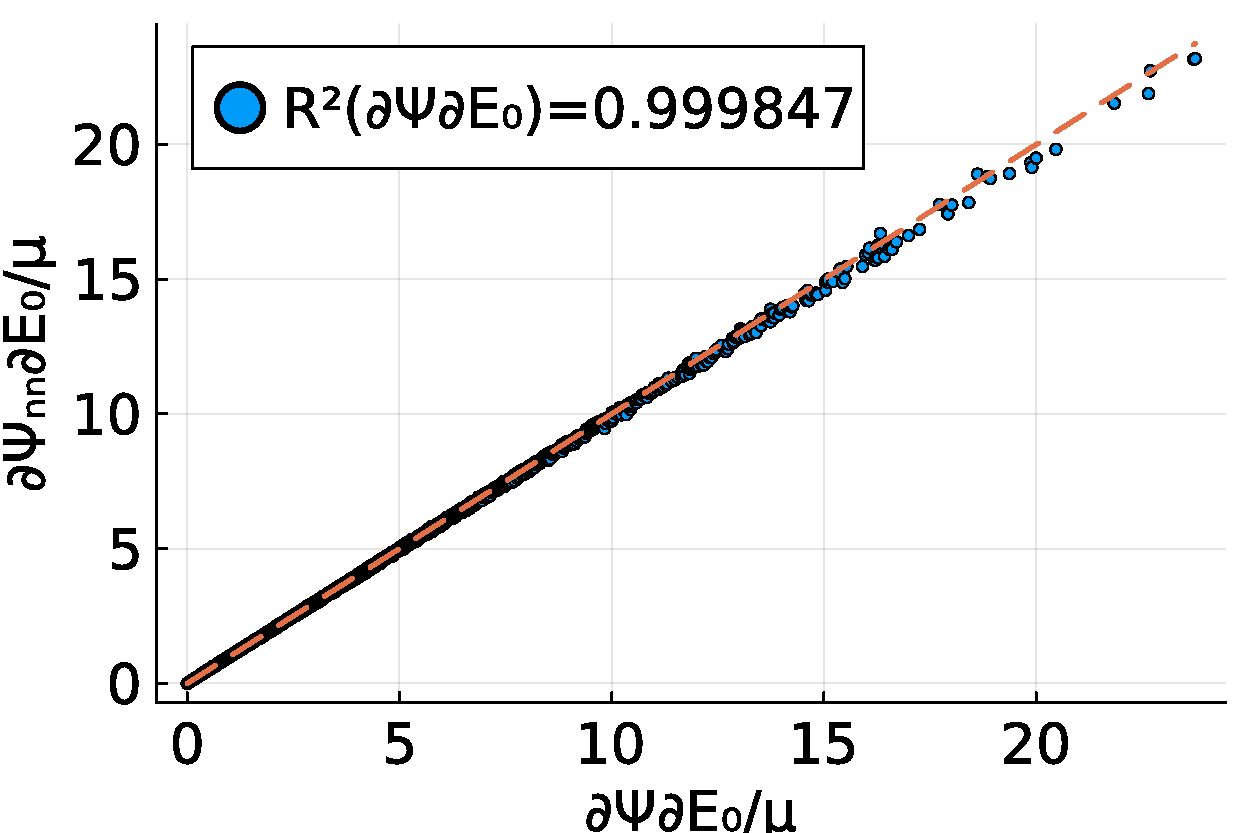
\includegraphics[width=0.33\textwidth]{Figures/ModelsStudy/_QuadraticMooneyRivlin_ID_E0_E0_CorrelationTest} &
		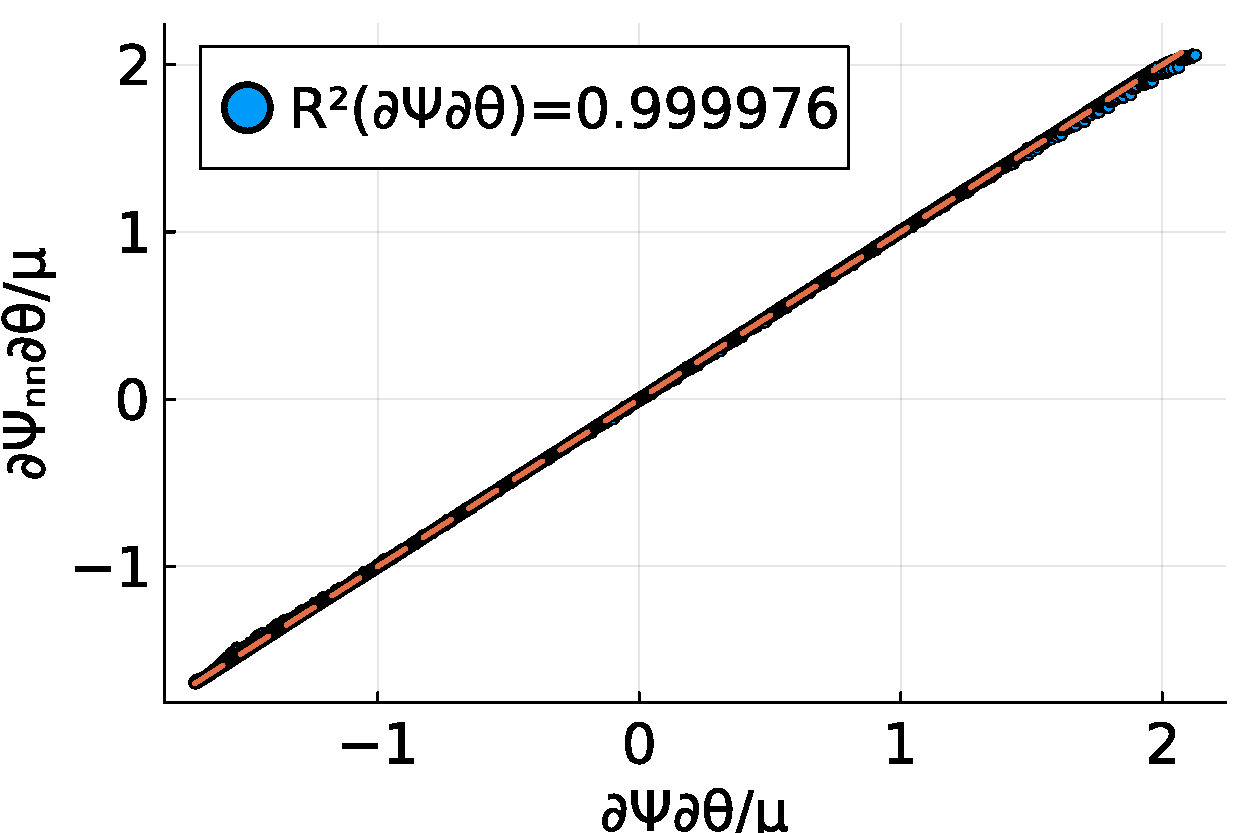
\includegraphics[width=0.33\textwidth]{Figures/ModelsStudy/_QuadraticMooneyRivlin_ID_E0_theta_CorrelationTest} \\
		%
		%
		\rotatebox{90}{\,\,\,\,\,\,\,\,\,\,\textcolor{red}{\textbf{Y}}/\textcolor{blue}{\textbf{ID}}}  &		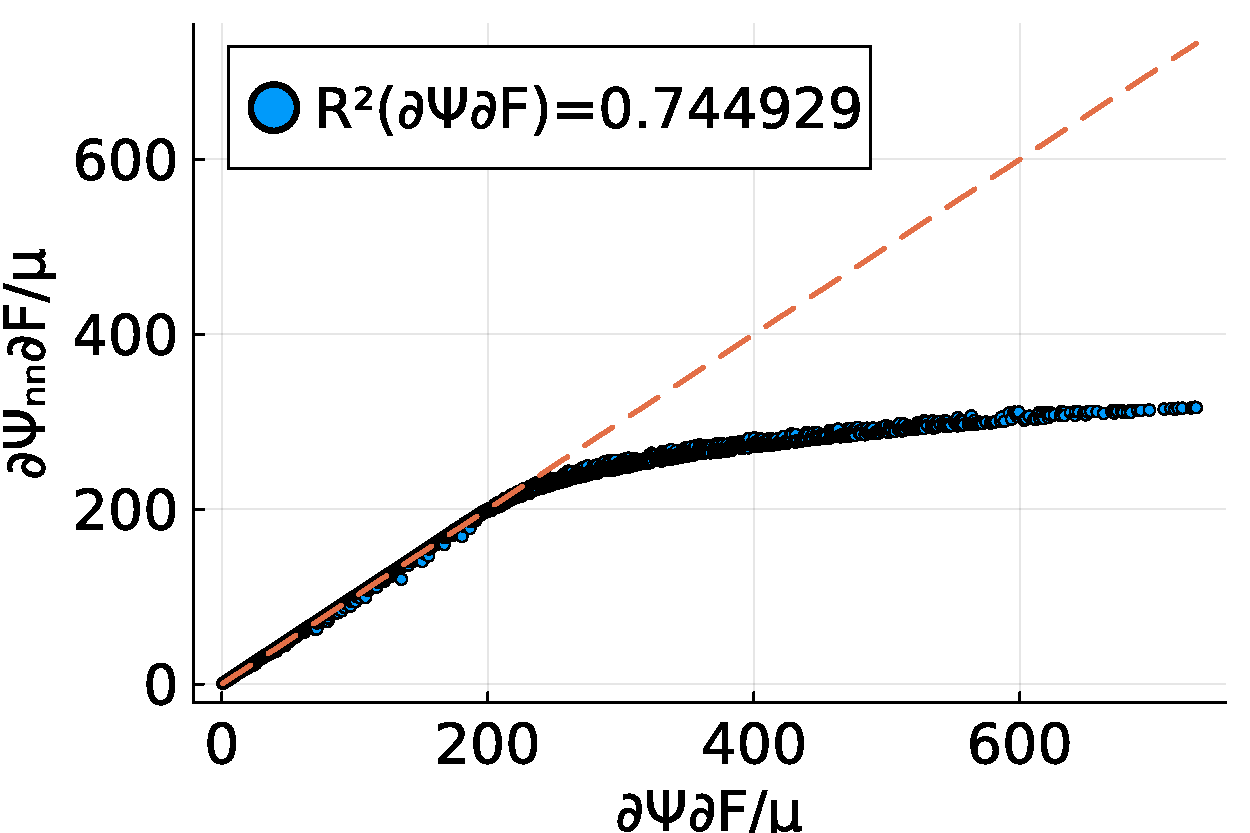
\includegraphics[width=0.33\textwidth]{Figures/ModelsStudy/_Yeoh_ID_E0_P_CorrelationTest} &
		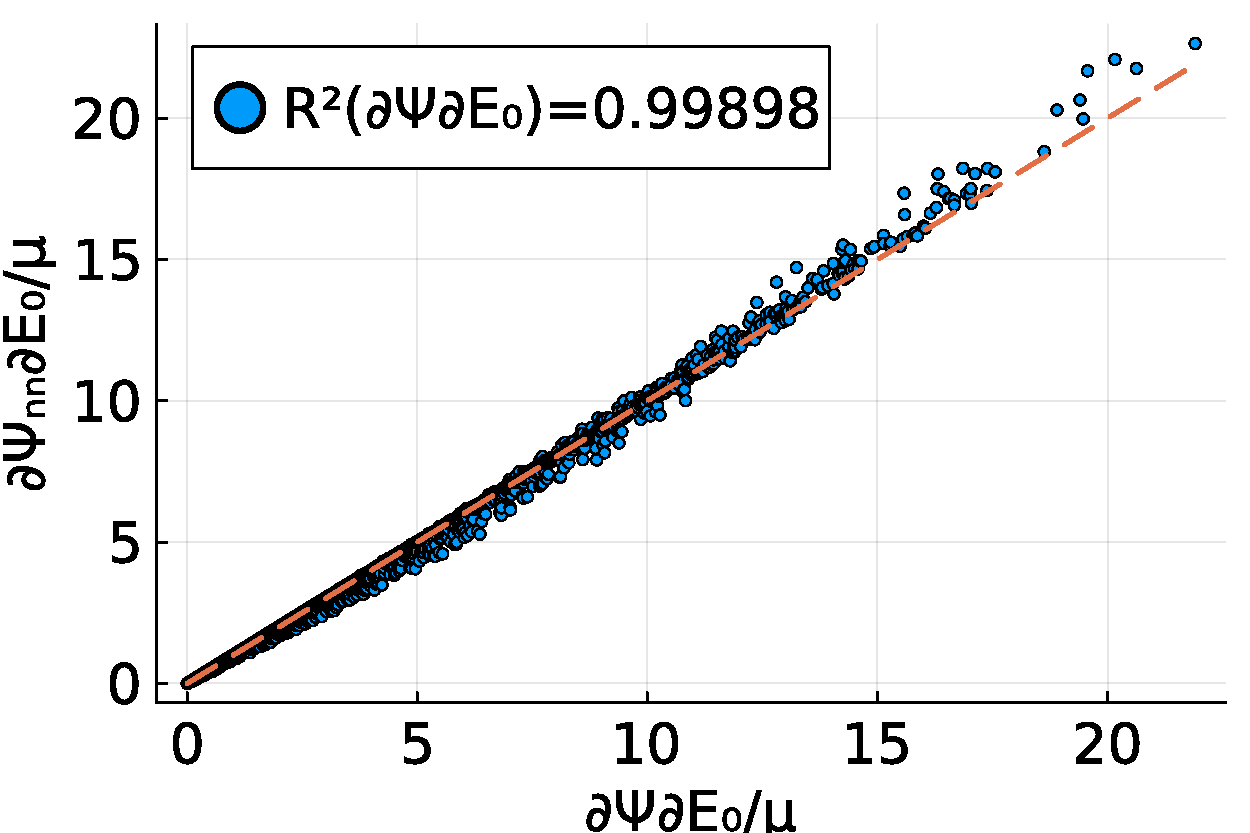
\includegraphics[width=0.33\textwidth]{Figures/ModelsStudy/_Yeoh_ID_E0_E0_CorrelationTest} &
		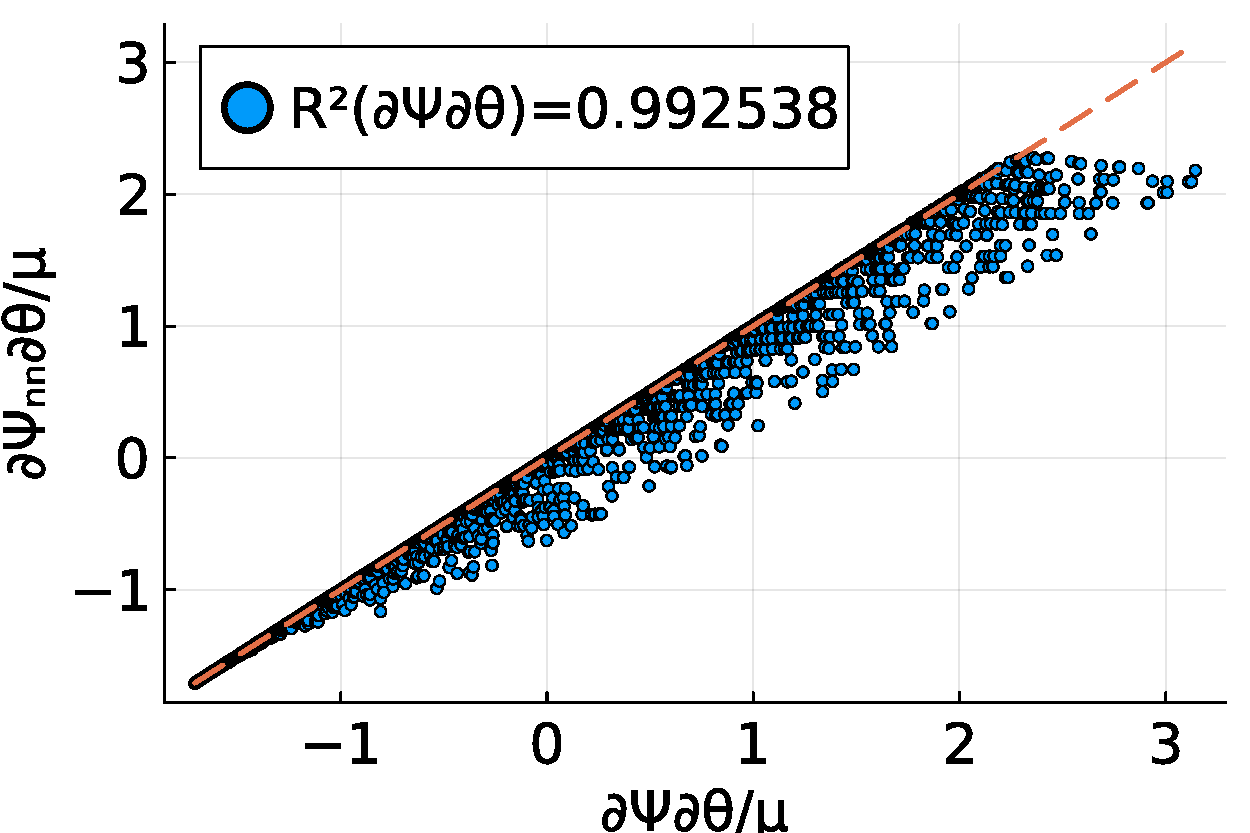
\includegraphics[width=0.33\textwidth]{Figures/ModelsStudy/_Yeoh_ID_E0_theta_CorrelationTest} \\
		%
		%
		\rotatebox{90}{\,\,\,\,\,\,\,\,\,\,\textcolor{red}{\textbf{G}}/\textcolor{blue}{\textbf{ID}}}  &		\includegraphics[width=0.33\textwidth]{Figures/ModelsStudy/_Gent_ID_E0_P_CorrelationTest} &
		\includegraphics[width=0.33\textwidth]{Figures/ModelsStudy/_Gent_ID_E0_E0_CorrelationTest} &
		\includegraphics[width=0.33\textwidth]{Figures/ModelsStudy/_Gent_ID_E0_theta_CorrelationTest} \\
		%
		%
		\rotatebox{90}{\,\,\,\,\,\,\,\,\,\,\textcolor{red}{\textbf{TI}}/\textcolor{blue}{\textbf{ID}}}  &		\includegraphics[width=0.33\textwidth]{Figures/ModelsStudy/_TI_ID_E0_P_CorrelationTest} &
		\includegraphics[width=0.33\textwidth]{Figures/ModelsStudy/_TI_ID_E0_E0_CorrelationTest} &
		\includegraphics[width=0.33\textwidth]{Figures/ModelsStudy/_TI_ID_E0_theta_CorrelationTest} \\
		%
		%
		\rotatebox{90}{\,\,\,\,\,\,\,\,\,\,\textcolor{red}{\textbf{MR}}/\textcolor{blue}{\textbf{ES}}}  &	\includegraphics[width=0.33\textwidth]{Figures/ModelsStudy/_MooneyRivlin_ElectricSaturation_P_CorrelationTest} &
		\includegraphics[width=0.33\textwidth]{Figures/ModelsStudy/_MooneyRivlin_ElectricSaturation_E0_CorrelationTest} &
		\includegraphics[width=0.33\textwidth]{Figures/ModelsStudy/_MooneyRivlin_ElectricSaturation_theta_CorrelationTest} \\
		%
		%
	\end{tabular}
	%
	%		\includegraphics[width=0.4\textwidth]{pictures_paper/inkscape_pictures/template_example_3.pdf}
	\caption{}
	\label{fig:example 1 energy balance}
\end{figure}



\clearpage

\subsubsection{Generalization results for $\Upsilon(\vect{F},\vect{D}_0,\theta)$}



\begin{figure}[hbtp]
	\centering
	\begin{tabular}{ccc}
		\includegraphics[width=0.33\textwidth]{Figures/PotentialStudy/Psi_P_CorrelationTest} &
		\includegraphics[width=0.33\textwidth]{Figures/PotentialStudy/Psi_E0_CorrelationTest} &
		\includegraphics[width=0.33\textwidth]{Figures/PotentialStudy/Psi_theta_CorrelationTest} \\
		%
		\includegraphics[width=0.33\textwidth]{Figures/PotentialStudy/e_P_CorrelationTest} &
		\includegraphics[width=0.33\textwidth]{Figures/PotentialStudy/e_E0_CorrelationTest} &
		\includegraphics[width=0.33\textwidth]{Figures/PotentialStudy/e_theta_CorrelationTest} \\		%	
		%	
		\includegraphics[width=0.33\textwidth]{Figures/PotentialStudy/Upsilon_P_CorrelationTest} &
		\includegraphics[width=0.33\textwidth]{Figures/PotentialStudy/Upsilon_E0_CorrelationTest} &
		\includegraphics[width=0.33\textwidth]{Figures/PotentialStudy/Upsilon_theta_CorrelationTest} \\		%	
		\includegraphics[width=0.33\textwidth]{Figures/PotentialStudy/Gamma_P_CorrelationTest} &
		\includegraphics[width=0.33\textwidth]{Figures/PotentialStudy/Gamma_E0_CorrelationTest} &
		\includegraphics[width=0.33\textwidth]{Figures/PotentialStudy/Gamma_theta_CorrelationTest} \\		
		
	\end{tabular}
	%
	%		\includegraphics[width=0.4\textwidth]{pictures_paper/inkscape_pictures/template_example_3.pdf}
	\caption{Numerical example 1. Evolution of: (a) angular momentum $\vect{J}$, (b) linear momentum $\vect{L}$, (c) global entropy $\tilde{\eta}=\int_{\mathcal{B}_0}\eta\,dV$, (d) Hamiltonian $\mathcal{H}$  in \eqref{eqn:Hamiltonian}, (e) increment of Hamiltonian $\Delta\mathcal{H}$ for both the Mid-Point and the new EM time integrator.  Finally, (f), zoomed detail of the increment of the Hamiltonian  $\Delta\mathcal{H}$ for the new EM time integrator. Results obtained for \textbf{Mesh2} with $\alpha_{CFL}=2.2955$ ($\Delta t=0.2$ s).}
	\label{fig:example 1 energy balance}
\end{figure}


\subsection{Calibration strategy 2: $\eta$-based potentials}


\subsubsection{Neural network architecture's influence: $e_{nn}$ neural network-based ground truth models}


\begin{table}[hbtp!]
	\centering
	\begin{tabular}{c c c c c c c c c c c c}
		\toprule
		\rowcolor{gray!30}	\small{} & $n_L+1$ & 1 &  2& 3& 4& 5& 1& 2& 3& 4 & 5\\
		\midrule 
		\rowcolor{gray!30}	\small{} & $n_n$ & 8 & 8& 8& 8 &8 &16& 16& 16& 16 &  16\\
		\midrule
		\multirow{3}{*}{\rotatebox{90}{\textcolor{red}{\textbf{MR}}/\textcolor{blue}{\textbf{ID}}}}  &$R^2(\partial_{\vect{F}}\Psi)$ & 1 & 1& 1 & 1 & 1& 1& 1& 1& 1 & 1\\
		&$R^2(\partial_{\vect{F}}\Psi)$ & 1 & 1& 1 & 1 & 1& 1& 1& 1& 1 & 1\\
		&$R^2(\partial_{\vect{F}}\Psi)$ & 1 & 1& 1 & 1 & 1& 1& 1& 1& 1 & 1\\	
		\midrule
		\multirow{3}{*}{\rotatebox{90}{\textcolor{red}{\textbf{QMR}}/\textcolor{blue}{\textbf{ID}}}} &$R^2(\partial_{\vect{F}}\Psi)$ & 1 & 1& 1 & 1 & 1& 1& 1& 1& 1 &  1\\
		&$R^2(\partial_{\vect{F}}\Psi)$ & 1 & 1& 1 & 1 & 1& 1& 1& 1& 1 &  1\\
		&$R^2(\partial_{\vect{F}}\Psi)$ & 1 & 1& 1 & 1 & 1& 1& 1& 1& 1 & 1\\	
		\\
		\midrule
		\multirow{3}{*}{\rotatebox{90}{\textcolor{red}{\textbf{Y}}/\textcolor{blue}{\textbf{ID}}}} &$R^2(\partial_{\vect{F}}\Psi)$ & 1 & 1& 1 & 1 & 1& 1& 1& 1& 1 &  1\\
		&$R^2(\partial_{\vect{F}}\Psi)$ & 1 & 1& 1 & 1 & 1& 1& 1& 1& 1 &  1\\
		&$R^2(\partial_{\vect{F}}\Psi)$ & 1 & 1& 1 & 1 & 1& 1& 1& 1& 1 & 1\\	
		\midrule
		\multirow{3}{*}{\rotatebox{90}{G/ID}} &$R^2(\partial_{\vect{F}}\Psi)$ & 1 & 1& 1 & 1 & 1& 1& 1& 1& 1 &  1\\
		&$R^2(\partial_{\vect{F}}\Psi)$ & 1 & 1& 1 & 1 & 1& 1& 1& 1& 1 &  1\\
		&$R^2(\partial_{\vect{F}}\Psi)$ & 1 & 1& 1 & 1 & 1& 1& 1& 1& 1 & 1\\	
		\midrule
		\multirow{3}{*}{\rotatebox{90}{TI/ID}} &$R^2(\partial_{\vect{F}}\Psi)$ & 1 & 1& 1 & 1 & 1& 1& 1& 1& 1 &  1\\
		&$R^2(\partial_{\vect{F}}\Psi)$ & 1 & 1& 1 & 1 & 1& 1& 1& 1& 1 &  1\\
		&$R^2(\partial_{\vect{F}}\Psi)$ & 1 & 1& 1 & 1 & 1& 1& 1& 1& 1 & 1\\	
		\midrule
		\multirow{3}{*}{\rotatebox{90}{MR/ES}} &$R^2(\partial_{\vect{F}}\Psi)$ & 1 & 1& 1 & 1 & 1& 1& 1& 1& 1 &  1\\
		&$R^2(\partial_{\vect{F}}\Psi)$ & 1 & 1& 1 & 1 & 1& 1& 1& 1& 1 &  1\\
		&$R^2(\partial_{\vect{F}}\Psi)$ & 1 & 1& 1 & 1 & 1& 1& 1& 1& 1 & 1\\	
		\midrule
	\end{tabular}
	\caption{}
	\label{table: results calibration strategy 1}
\end{table}


\clearpage



\begin{figure}[hbtp!]
	\centering
	\begin{tabular}{cccc}
		\rotatebox{90}{\,\,\,\,\,\,\,\,\,\,\textcolor{red}{\textbf{MR}}/\textcolor{blue}{\textbf{ID}}}  &		\includegraphics[width=0.33\textwidth]{Figures/ModelsStudy/_MooneyRivlin_ID_E0_P_CorrelationTest} &
		\includegraphics[width=0.33\textwidth]{Figures/ModelsStudy/_MooneyRivlin_ID_E0_E0_CorrelationTest} &
		\includegraphics[width=0.33\textwidth]{Figures/ModelsStudy/_MooneyRivlin_ID_E0_theta_CorrelationTest} %\\
		%
%		\rotatebox{90}{\,\,\,\,\,\,\,\,\,\,\textcolor{red}{\textbf{QMR}}/\textcolor{blue}{\textbf{ID}}} &	\includegraphics[width=0.33\textwidth]{Figures/ModelsStudy/_QuadraticMooneyRivlin_ID_E0_P_CorrelationTest} &
%		\includegraphics[width=0.33\textwidth]{Figures/ModelsStudy/_QuadraticMooneyRivlin_ID_E0_E0_CorrelationTest} &
%		\includegraphics[width=0.33\textwidth]{Figures/ModelsStudy/_QuadraticMooneyRivlin_ID_E0_theta_CorrelationTest} \\
		%
		%
%		\rotatebox{90}{\,\,\,\,\,\,\,\,\,\,\textcolor{red}{\textbf{Y}}/\textcolor{blue}{\textbf{ID}}}  &		\includegraphics[width=0.33\textwidth]{Figures/ModelsStudy/_Yeoh_ID_E0_P_CorrelationTest} &
%		\includegraphics[width=0.33\textwidth]{Figures/ModelsStudy/_Yeoh_ID_E0_E0_CorrelationTest} &
%		\includegraphics[width=0.33\textwidth]{Figures/ModelsStudy/_Yeoh_ID_E0_theta_CorrelationTest} \\
		%
		%
%		\rotatebox{90}{\,\,\,\,\,\,\,\,\,\,\textcolor{red}{\textbf{G}}/\textcolor{blue}{\textbf{ID}}}  &		\includegraphics[width=0.33\textwidth]{Figures/ModelsStudy/_Gent_ID_E0_P_CorrelationTest} &
%		\includegraphics[width=0.33\textwidth]{Figures/ModelsStudy/_Gent_ID_E0_E0_CorrelationTest} &
%		\includegraphics[width=0.33\textwidth]{Figures/ModelsStudy/_Gent_ID_E0_theta_CorrelationTest} \\
%		%
%		%
%		\rotatebox{90}{\,\,\,\,\,\,\,\,\,\,\textcolor{red}{\textbf{TI}}/\textcolor{blue}{\textbf{ID}}}  &		\includegraphics[width=0.33\textwidth]{Figures/ModelsStudy/_TI_ID_E0_P_CorrelationTest} &
%		\includegraphics[width=0.33\textwidth]{Figures/ModelsStudy/_TI_ID_E0_E0_CorrelationTest} &
%		\includegraphics[width=0.33\textwidth]{Figures/ModelsStudy/_TI_ID_E0_theta_CorrelationTest} \\
%		%
%		%
%		\rotatebox{90}{\,\,\,\,\,\,\,\,\,\,\textcolor{red}{\textbf{MR}}/\textcolor{blue}{\textbf{ES}}}  &	\includegraphics[width=0.33\textwidth]{Figures/ModelsStudy/_MooneyRivlin_ElectricSaturation_P_CorrelationTest} &
%		\includegraphics[width=0.33\textwidth]{Figures/ModelsStudy/_MooneyRivlin_ElectricSaturation_E0_CorrelationTest} &
%		\includegraphics[width=0.33\textwidth]{Figures/ModelsStudy/_MooneyRivlin_ElectricSaturation_theta_CorrelationTest} \\
		%
		%
	\end{tabular}
	%
	%		\includegraphics[width=0.4\textwidth]{pictures_paper/inkscape_pictures/template_example_3.pdf}
	\caption{}
	\label{fig:example 1 energy balance}
\end{figure}







\clearpage

\subsection{Finite Element numerical experiments}

The objective of this section is to study the performance of the newly proposed EM time integration scheme presented in equation \eqref{eqn:weak forms for proposed time integrator} in a variety of challenging examples, {with the aim of comparing the long-term stability of the new time integrator against that of the classical midpoint rule.}



\subsubsection{Numerical Example 1}


The objectives of this example are:
%
\begin{itemize}

\item \textbf{O1} To carry out a thorough analysis of the stability and robustness of the proposed EM time integrator comparing it against of the mid-point rule time integrator  as a function of the Courant-Friedrich-Lewy number for the case of Finite Element $h$-refinement. 

\item \textbf{O2}   For a given level of spatial discretisation refinement and time step, to compare the thermodynamical consistency of the proposed time integrator to that of the mid-point time integrator.


\end{itemize}	

The geometry for the problem is displayed in Figure \ref{fig:LShape geometry}. The L-shaped solid is subjected to an external torque induced by a pair of forces $\vect{F}_1(t)$ and $\vect{F}_2(t)$ acting on two of the boundary faces (refer to Figure \ref{fig:LShape geometry}), defined as
%
\begin{equation}\label{eqn:Torque}
\vect{F}_2(t)=-\vect{F}_1(t);\qquad
\vect{F}_1(t)=\begin{bmatrix}
256/9\\512/9\\768/9
\end{bmatrix}f(t);\qquad f(t)=\left\{\begin{array}{ccc}
\begin{aligned}
t&&0\leq t<2.5\,\text{s} ,\\
5-t&&2.5\,\text{s}\leq t<5\,\text{s}\\
0  &&t\geq 5\,\text{s}. 
\end{aligned} 
\end{array}\right.
\end{equation}

In addition, initial distribution of temperature on the solid is
%
\begin{equation}
\left.\theta(\vect{X})\right\vert_{t=0}=\left\{\begin{array}{ccc}
\begin{aligned}
T_1&&Z=L_Z ,\\
T_2&&X=L_X\\
\theta_R  &&\text{elsewhere}. 
\end{aligned} 
\end{array}\right.;\qquad
T_1=300\,K; \qquad  T_2=250\,K.
\end{equation} 


\begin{figure}[hbtp]
	\centering
	\includegraphics[width=0.3\textwidth]{Figures/Example1/LShape.pdf}
	%
	%		\includegraphics[width=0.4\textwidth]{pictures_paper/inkscape_pictures/template_example_3.pdf}
	\caption{Numerical example 1. Geometry and general setting.}
	\label{fig:LShape geometry}
\end{figure}
%


In order to establish a quantitative comparison with the results provided in Reference \cite{Betsch2018Thermo}, we use in this example the  constitutive model considered therein. This can be expressed in terms of the following additive decomposition,
%
\begin{equation}\label{eqn:Betsch model}
\begin{aligned}
\widetilde{W}\left(\vect{C},\vect{G},C,\theta\right)& = \widetilde{W}_{m}\left(\vect{C},\vect{G},C\right) + \widetilde{W}_{\theta}\left(\theta\right) - 
{(\theta-\theta_R)\widetilde{\eta}_R\left(C\right)},
\end{aligned}
\end{equation}
%
where each of the contributions in \eqref{eqn:Betsch model} is defined as
%
\begin{equation}\label{eqn:Betsch model II}
\begin{aligned}
 \widetilde{W}_{m}\left(\vect{C},\vect{G},C\right)&= \frac{\mu_1}{2}\text{tr}\vect{C} + \frac{\mu_2}{2}\text{tr}\vect{G} - \left(\mu_1 + 2\mu_2\right)\ln C^{1/2} + \frac{\lambda}{2}\left(C^{1/2}-1\right)^2;\\
 %
 \widetilde{W}_{\theta}(\theta)&=c_v\left(\theta - \theta_R - \theta \ln\frac{\theta}{\theta_R}\right);\quad
 %
 \widetilde{\eta}_R(C) = -3\beta\left(a(C^{1/2}-1) - bC^{-1/2}\right).
\end{aligned}
\end{equation}

The thermal conductivity tensor is particularised for the case of isotropy, whereby it can be expressed in terms of the scalar conductivity field $k$, i.e. $\vect{k} = k\vect{I}$. The value of all the relevant material and geometrical parameters in this example can be found in Table \ref{table:LShape parameters}.

\begin{table}[htbp]
	\centering
	\caption{Numerical example 1. Geometrical parameters (see Figure \ref{fig:LShape geometry}) and material parameters (see \eqref{eqn:Betsch model II}).}
	%
	\label{table:LShape parameters}
	%
	\vspace{2mm}
	\begin{tabular}{l | c c c l|}
		%\hline
		\cellcolor{gray!15}&&&&\\
		\cellcolor{gray!15}\textbf{Geometrical parameters}  &  $L_X$ &  6  &  m  &		\\
		%
		\cellcolor{gray!15}  &  $L_Y$ & 3 & m &\\
		%
		\cellcolor{gray!15}	&  $L_Z$ & 10 & m &\\
		%
		\hline
		%
		\cellcolor{gray!15}&&&\\
		\cellcolor{gray!15}\textbf{Material parameters}  &  $\mu_1$ &  1646,7  &  Pa &
		\\
		%
		\cellcolor{gray!15}&  $\mu_2$ & 332,5 & Pa &\\ %
		\cellcolor{gray!15}&  $\lambda$ & 0 & Pa &\\
		\cellcolor{gray!15}&  $c_v$ & 100 & $\text{J}\text{K}^{-1}\text{m}^{-3}$& \textit{(Specific heat capacity)}\\
		\cellcolor{gray!15}&  $\theta_R$ & 293.15 & K& \textit{(Reference temperature)}\\
		\cellcolor{gray!15}&  $\beta$ & $2,233\times10^{-4}$ & K$^{-1}$&\\
		\cellcolor{gray!15}&  $a$ & $\mu_1+  2\mu_2$ & Pa&\\
		\cellcolor{gray!15}&  $b$ & 0 & Pa&\\
		\cellcolor{gray!15}&  $k$ & 10 & WK$^{-1}$m$^{-1}$& \textit{(Thermal conductivity)}\\	
		\cellcolor{gray!15}&  $\rho_0$ & 100 & kg/$\text{m}^3$& \textit{(Material density)}\\				
		%
		%\hline
	\end{tabular}
\end{table}


\begin{figure}[hbtp]
	\centering
	\includegraphics[width=0.85\textwidth]{Figures/Example1/Meshesv2.pdf}
	%
	%		\includegraphics[width=0.4\textwidth]{pictures_paper/inkscape_pictures/template_example_3.pdf}
	\caption{Numerical example 1. $h$-refinement used in the study. $Q_1$-$Q_1$ finite element discretisation for both spatial geometry $\vect{\phi}$ and temperature $\theta$. From left to right: \textbf{Mesh1} (with $\{672,224\}$ dofs for $\{\vect{\phi},\theta\}$); \textbf{Mesh2} (refinement of $\times 2$ in every direction with respect to \textbf{Mesh1}, yielding $\{3822,1274\}$ dofs for $\{\vect{\phi},\theta\}$); \textbf{Mesh3} (refinement of $\times 3$ in every direction with respect to \textbf{Mesh1}, yielding $\{12000,4000\}$ dofs for $\{\vect{\phi},\theta\}$); \textbf{Mesh4} (refinement of $\times 4$ in every direction with respect to \textbf{Mesh1}, yielding $\{25350,8450\}$ dofs for $\{\vect{\phi},\theta\}$).}
	\label{fig:LShape meshes}
\end{figure}
%

Four different levels of $h$-refinement will be considered in this example. These can be observed in Figure \ref{fig:LShape meshes}. A course, medium,  fine and ulta fine finite element meshes (denoted as \textbf{Mesh1}, \textbf{Mesh2}, \textbf{Mesh3} and \textbf{Mesh4}, respectively) have been considered. With regards to objective $\textbf{O1}$,  we recall that the Courant-Friedrichs-Lewy number (denoted hereby as $\alpha_{CFL}$) is defined as
%
\begin{equation}\label{eqn:CFL}
\alpha_{CFL}=c_p\frac{\Delta t}{h};\qquad c_p=\sqrt{\frac{\lambda_R + 2\mu_R}{\rho_0}},
\end{equation}
%
where $\Delta t$ denotes the time step used in the simulations and $h$ the characteristic size of the finite element mesh, and $c_p$ the longitudinal wave speed in the reference configuartion ($\vect{\nabla}_0\vect{\phi}=\vect{I},\,\theta=\theta_R$). For hexahedral meshes, we consider $h$ to be related to the volume of the element $e$ in the mesh  (i.e. $V_e$) and to the order of the Finite Element interpolation $q$ (i.e. $q=1$ for $Q_1$ elements, $q=2$ for $Q_2$ elements, etc.) as
%
\begin{equation}
h = \left(\frac{\min\limits_{e}V_{e}}{q^3}\right)^{1/3};\qquad 1\leq e \leq N, 
\end{equation}
%
where $N$ denotes the number of elements for the underlying discretisation. 
%In addition, in \eqref{eqn:CFL}, $\{\mu_R,\lambda_R\}$ represent the shear and bulk moduli of the material in the origin (see equation \eqref{eqn:reference mechanical properties}). 
Figure \ref{fig:CFL study}$_a$ shows the final time instant $T_{final}$ for which the proposed EM time integrator fails, that is, \Blue{the time step for which the convergence of the iterative Netwon-Raphson algorithm is not achieved \cite{Kuhl_Crisfield_1996,Kuhl_Crisfield_1999}}, for different values of the $\alpha_{CFL}$ number and for the four levels of $h$-refinement displayed in Figure \ref{fig:LShape meshes}. Clearly, for large values of the $\alpha_{CFL}$ number, the new EM time integrator becomes unstable at smaller values of $T_{final}$, as expected. 


Figure \ref{fig:CFL study}$_b$ sheds light with regards to the relative stability of the proposed EM time integrator with respect to that of the classical mid-point time integrator. Specifically, this figure shows the difference between the final time instant for which the proposed EM time integrator and the mid-point rule become unstable. This has been denoted in that figure as $\Delta T_{final}$. \Blue{Contrary to the EM time integrator, for the mid-point integrator, the lack of convergence of the Newton-Raphson is always preceded by an uncontrollable growth of the Hamiltonian over the previous time steps.} Positive values of $\Delta T_{final}$ imply that the proposed time integrator becomes unstable at later time instants, and viceversa. It is worth noticing that beyond $\alpha_{CFL}\geq 5-10$,  $\Delta T_{final}$ adopts negative values. This indicates that the size of the time step $\Delta t$ cannot be chosen arbitrarily large, expecting an improved robustness and stability of the EM time integrator with respect to the classical mid-point rule. In fact our numerical study suggests that $\Delta t$ must be chosen such that $\alpha_{CFL}\leq 5$ in order to guarantee a higher stability and robustness in the long term.



\begin{figure}[hbtp]
	\centering
	\begin{tabular}{cc}
	\includegraphics[width=0.5\textwidth]{Figures/Example1/Tfinalv4.eps} &
%	\includegraphics[width=0.5\textwidth]{Figures/Example1/Tfinalv4.eps}
\includegraphics[width=0.5\textwidth]{Figures/Example1/DTfinalv4.eps}
	\end{tabular}
	%
	%		\includegraphics[width=0.4\textwidth]{pictures_paper/inkscape_pictures/template_example_3.pdf}
	\caption{Numerical example 1. Left: final time instant ($T_{final}$) for which the EM time integrator becomes unstable. Rigth: Difference between the final time instant ($\Delta T_{final}$) at which the EM time integrator and the mid-point rule become unstable. Results shown for various values of $\alpha_{CFL}$ and for the discretisations in Figure \ref{fig:LShape meshes}.}
	\label{fig:CFL study}
\end{figure}


\begin{figure}[hbtp]
	\centering
	\begin{tabular}{cc}
		\includegraphics[width=0.5\textwidth]{Figures/Example1/EnergyBalancePlots/Jv2.eps} &
		\includegraphics[width=0.5\textwidth]{Figures/Example1/EnergyBalancePlots/LinearMomentumv2.eps}\\
		%
	\includegraphics[width=0.5\textwidth]{Figures/Example1/EnergyBalancePlots/EntropyFinalv2.eps} &
\includegraphics[width=0.5\textwidth]{Figures/Example1/EnergyBalancePlots/EnergyFinalv2.eps}\\
%
	\includegraphics[width=0.5\textwidth]{Figures/Example1/EnergyBalancePlots/DHFinalv2.eps} &
\includegraphics[width=0.5\textwidth]{Figures/Example1/EnergyBalancePlots/DHEMv2.eps}\\
%		
	\end{tabular}
	%
	%		\includegraphics[width=0.4\textwidth]{pictures_paper/inkscape_pictures/template_example_3.pdf}
	\caption{Numerical example 1. Evolution of: (a) angular momentum $\vect{J}$, (b) linear momentum $\vect{L}$, (c) global entropy $\tilde{\eta}=\int_{\mathcal{B}_0}\eta\,dV$, (d) Hamiltonian $\mathcal{H}$  in \eqref{eqn:Hamiltonian}, (e) increment of Hamiltonian $\Delta\mathcal{H}$ for both the Mid-Point and the new EM time integrator.  Finally, (f), zoomed detail of the increment of the Hamiltonian  $\Delta\mathcal{H}$ for the new EM time integrator. Results obtained for \textbf{Mesh2} with $\alpha_{CFL}=2.2955$ ($\Delta t=0.2$ s).}
	\label{fig:example 1 energy balance}
\end{figure}


With regards to objective \textbf{O2}, we use in this study the computational domain defined by \textbf{Mesh2} (see Figure \ref{fig:LShape meshes}) and a value of $\alpha_{CFL}$ of $\alpha_{CFL}=2.2955$. It can be seen that for both the new EM time integrator and the mid-point rule the angular momentum $\vect{J}$ remains constant beyond $t\geq 5\,\textbf{s}$, when the external applied pair of forces vanishes. In addition, the linear momentum $\vect{L}$ is zero for the entire simulation. Another interesting variable of interest is the global entropy ($\tilde{\eta}=\int_{\mathcal{B}_0}\eta\,dV$), which increases over time for the entire simulation for both time integrators. Furthermore, the Hamiltonian $\mathcal{H}$ is displayed. The zoomed detail perfectly shows the sudden increase in the Hamiltonian $\mathcal{H}$ prior to the instability when using the mid-point rule. The increase of the Hamiltonian $\Delta \mathcal{H}={\mathcal{H}_{n+1}-\mathcal{H}_n}$ (normalised with respect to the maximum historic value of $\mathcal{H}$ in absolute value) is also displayed. It can be seen that the new EM time integrator preserves $\mathcal{H}$ (beyond $t\geq 5\,\text{s}$) as it has been designed specifically with that purpose, whereas the mid-point rule does not. 

Finally, the temperature contour plot is displayed over time in Figure \ref{fig:example 1 temperature}. The results have been obtained by means of the new EM time integrator using a different mesh from the four depicted in Figure \ref{fig:LShape meshes}. This mesh has been generated refining by a factor of $\times 6$ in the three directions the computational domain defined by \textbf{Mesh1}.



%\begin{figure}[hbtp]
%	\centering
%	\begin{tabular}{ccc}
%		\includegraphics[width=0.26\textwidth]{Figures/Example1/Pressure/RainBowBright/PressureNoMeshTimeStep25v2} &
%		\includegraphics[width=0.24\textwidth]{Figures/Example1/Pressure/RainBowBright/PressureNoMeshTimeStep50v2}
%		\includegraphics[width=0.40\textwidth]{Figures/Example1/Pressure/RainBowBright/PressureNoMeshTimeStep80v2} 
%		\\
%		\includegraphics[width=0.35\textwidth]{Figures/Example1/Pressure/RainBowBright/PressureNoMeshTimeStep110v2} &
%		\includegraphics[width=0.26\textwidth]{Figures/Example1/Pressure/RainBowBright/PressureNoMeshTimeStep150v2}
%		\includegraphics[width=0.36\textwidth]{Figures/Example1/Pressure/RainBowBright/PressureNoMeshTimeStep190v2} 
%		\\
%		\includegraphics[width=0.36\textwidth]{Figures/Example1/Pressure/RainBowBright/PressureNoMeshTimeStep210v2} &
%\includegraphics[width=0.24\textwidth]{Figures/Example1/Pressure/RainBowBright/PressureNoMeshTimeStep250v2}
%\includegraphics[width=0.24\textwidth]{Figures/Example1/Pressure/RainBowBright/PressureNoMeshTimeStep330v2} 		\\
%%
%		\includegraphics[width=0.25\textwidth]{Figures/Example1/Pressure/RainBowBright/PressureNoMeshTimeStep350v2} &
%\includegraphics[width=0.36\textwidth]{Figures/Example1/Pressure/RainBowBright/PressureNoMeshTimeStep400v2}
%\includegraphics[width=0.25\textwidth]{Figures/Example1/Pressure/RainBowBright/PressureNoMeshTimeStep430v2} 		
%	\end{tabular}
%	%
%	%		\includegraphics[width=0.4\textwidth]{pictures_paper/inkscape_pictures/template_example_3.pdf}
%	\caption{Numerical example 1. XX.}
%	\label{fig:example 1 pressure}
%\end{figure}
%%



%\begin{figure}[hbtp]
%	\centering
%	\begin{tabular}{ccc}
%		\includegraphics[width=0.21\textwidth]{Figures/Example1/Pressure/JetColor/PressureNoMeshJetTimeStep25v2} &
%		\includegraphics[width=0.17\textwidth]{Figures/Example1/Pressure/JetColor/PressureNoMeshJetTimeStep50v2}
%		\includegraphics[width=0.35\textwidth]{Figures/Example1/Pressure/JetColor/PressureNoMeshJetTimeStep80v2} 
%		\\
%		\includegraphics[width=0.30\textwidth]{Figures/Example1/Pressure/JetColor/PressureNoMeshJetTimeStep110v2} &
%		\includegraphics[width=0.21\textwidth]{Figures/Example1/Pressure/JetColor/PressureNoMeshJetTimeStep150v2}
%		\includegraphics[width=0.33\textwidth]{Figures/Example1/Pressure/JetColor/PressureNoMeshJetTimeStep190v2} 
%		\\
%		\includegraphics[width=0.29\textwidth]{Figures/Example1/Pressure/JetColor/PressureNoMeshJetTimeStep210v2} &
%		\includegraphics[width=0.19\textwidth]{Figures/Example1/Pressure/JetColor/PressureNoMeshJetTimeStep250v2}
%		\includegraphics[width=0.19\textwidth]{Figures/Example1/Pressure/JetColor/PressureNoMeshJetTimeStep330v2} 		\\
%		%
%		\includegraphics[width=0.20\textwidth]{Figures/Example1/Pressure/JetColor/PressureNoMeshJetTimeStep350v2} &
%		\includegraphics[width=0.31\textwidth]{Figures/Example1/Pressure/JetColor/PressureNoMeshJetTimeStep400v2}
%		\includegraphics[width=0.22\textwidth]{Figures/Example1/Pressure/JetColor/PressureNoMeshJetTimeStep430v2} 		
%	\end{tabular}
%%
%		\includegraphics[width=0.5\textwidth]{Figures/Example1/Pressure/JetColor/ColorBar} 		
%	%
%	%		\includegraphics[width=0.4\textwidth]{pictures_paper/inkscape_pictures/template_example_3.pdf}
%	\caption{Numerical example 1. XX.}
%	\label{fig:example 1 pressure}
%\end{figure}


%\begin{figure}[hbtp]
%	\centering
%	\begin{tabular}{ccc}
%		\includegraphics[width=0.21\textwidth]{Figures/Example1/Temperature/TimeStep25v2} &
%		\includegraphics[width=0.17\textwidth]{Figures/Example1/Temperature/TimeStep50v2}
%		\includegraphics[width=0.35\textwidth]{Figures/Example1/Temperature/TimeStep80v2} 
%		\\
%		\includegraphics[width=0.30\textwidth]{Figures/Example1/Temperature/TimeStep110v2} &
%		\includegraphics[width=0.21\textwidth]{Figures/Example1/Temperature/TimeStep150v2}
%		\includegraphics[width=0.33\textwidth]{Figures/Example1/Temperature/TimeStep190v2} 
%		\\
%		\includegraphics[width=0.29\textwidth]{Figures/Example1/Temperature/TimeStep210v2} &
%		\includegraphics[width=0.19\textwidth]{Figures/Example1/Temperature/TimeStep250v2}
%		\includegraphics[width=0.19\textwidth]{Figures/Example1/Temperature/TimeStep330v2} 		\\
%		%
%		\includegraphics[width=0.20\textwidth]{Figures/Example1/Temperature/TimeStep350v2} &
%		\includegraphics[width=0.31\textwidth]{Figures/Example1/Temperature/TimeStep400v2}
%		\includegraphics[width=0.22\textwidth]{Figures/Example1/Temperature/TimeStep430v2} 		
%	\end{tabular}
%	%
%		\includegraphics[width=0.5\textwidth]{Figures/Example1/Temperature/ColorBar} 			
%	%		\includegraphics[width=0.4\textwidth]{pictures_paper/inkscape_pictures/template_example_3.pdf}
%	\caption{Numerical example 1. XX.}
%	\label{fig:example 1 pressure}
%\end{figure}



\begin{figure}[hbtp]
	\centering
	\begin{tabular}{ccc}
		\includegraphics[width=0.12\textwidth]{Figures/Example1/Temperature/TS25v2} &
		\includegraphics[width=0.13\textwidth]{Figures/Example1/Temperature/TS50v2} &
		\includegraphics[width=0.27\textwidth]{Figures/Example1/Temperature/TS80v2} \\
		\includegraphics[width=0.23\textwidth]{Figures/Example1/Temperature/TS110v2} &
		\includegraphics[width=0.15\textwidth]{Figures/Example1/Temperature/TS150v2} &
		\includegraphics[width=0.26\textwidth]{Figures/Example1/Temperature/TS190v2} \\ 	
		\includegraphics[width=0.22\textwidth]{Figures/Example1/Temperature/TS210v2} &
		\includegraphics[width=0.12\textwidth]{Figures/Example1/Temperature/TS250v2}&
		%
		\includegraphics[width=0.12\textwidth]{Figures/Example1/Temperature/TS330v2}\\ 				
		%
		\includegraphics[width=0.16\textwidth]{Figures/Example1/Temperature/TS350v2} &
		\includegraphics[width=0.25\textwidth]{Figures/Example1/Temperature/TS400v2} &
		\includegraphics[width=0.13\textwidth]{Figures/Example1/Temperature/TS430v2} 		
	\end{tabular}
	%
	\includegraphics[width=0.5\textwidth]{Figures/Example1/Temperature/TSColorBarv2} 			
	%		\includegraphics[width=0.4\textwidth]{pictures_paper/inkscape_pictures/template_example_3.pdf}
	\vspace{-2mm}
	%
	\caption{Numerical example 1. Contour plot distribution of absolute temperature $T(K)$ for $t=\{2.5,5,8,11,15,19,21,25,33,35,40,43\}\,\text{s}$ (from left to right and top to bottom). $Q_1$-$Q_1$ discretisation for both spatial geometry $\vect{\phi}$ and temperature $\theta$. Number of dofs in the mesh: $\{85557,28519\}$ for $\{\vect{\phi},\theta\}$. Results obtained by means of the new EM time integrator for $\alpha_{CFL}=3.44$ ($\Delta t = 0.1\,\text{s}$).}
	\label{fig:example 1 temperature}
\end{figure}




\newpage


\subsection{Numerical Example 2}

The objective of this example is

\begin{itemize}
	\item \textbf{O1}   Study the stability and robustness in a problem where the deformation is exclusively induced by thermal effects.
	
\end{itemize}	

The geometry for this example is displayed in Figure \ref{fig:Bending actuator geometry}. The object in Figure \ref{fig:Bending actuator geometry} is  subjected to a heat flux at the bottom surface (minimum coordinate $Z$),  characterised by the following mathematical expression
%
\begin{equation}\label{eqn:Heat Flux}
Q_{\theta}(t)=Q_{\text{max}}\sin{\frac{2\pi}{T}t};\qquad T=1\,\text{s};\qquad Q_{\text{max}}=3000\,\mathrm{{W/m^2}}.
\end{equation}


\begin{figure}[hbtp]
	\centering
	\includegraphics[width=0.9\textwidth]{Figures/Example3/TheActuatorAndMeshForStudy.eps}
	%	\begin{tabular}{cc}
	%	\includegraphics[width=0.7\textwidth]{Figures/Example3/TheActuator.eps}&
	%    \includegraphics[width=0.3\textwidth]{Figures/Example3/MeshForStudy}
	%	\end{tabular}
	%
	%		\includegraphics[width=0.4\textwidth]{pictures_paper/inkscape_pictures/template_example_3.pdf}
	\caption{Numerical example 2. Left: geometry and general setting for the bi-material thermo-mechanical actuator. Right: computational domain considered for the analysis of $\textbf{O1}$, based on a  $Q_2$ discretisation for $\{\vect{x},T\}$, ($\{1215,405\}$ dofs). Every $Q_2$ finite element has been divided into $2\times 2\times 2$ elements for visualisation purposes.}
	\label{fig:Bending actuator geometry}
\end{figure}
%

The constitutive model used in this example is that presented in Section \ref{sec:constitutive models} through equations \eqref{eqn:additive decomposition}, \eqref{eqn:MRv2}, \eqref{eqn:thermal contribution} and \eqref{eqn:coupled contribution}. The value of the material parameters in that model can be found in {Table \ref{table:Bending actuator parameters}}.
%\begin{equation}
%\begin{aligend}
%\vect{v} = 20\sqrt{\frac{\pi}{2}}
%\end{aligned}
%\end{equation}

\begin{table}[htbp]
	\centering
	\caption{Numerical example 2. Geometrical parameters (see Figure \Blue{\ref{fig:Bending actuator geometry}}) and material parameters (see \eqref{eqn:Betsch model II}).}
	%
	\label{table:Bending actuator parameters}
	%
	\vspace{2mm}
	\begin{tabular}{l | c c c l|}
		%\hline
		\cellcolor{gray!15}&&&&\\
		\cellcolor{gray!15}\textbf{Geometrical parameters}  &  $L$ &  0,12  &  m  &		\\
		%
		\cellcolor{gray!15} &  $b$ & 0,06 & m &\\
		\cellcolor{gray!15} &  $H$ & 0,001 & m &\\		
		%
		\cellcolor{gray!15}&  $R$ & 0,01 & m &\\
		%
		\hline
		%
		\cellcolor{gray!15}&&&\\
		%%%%%%%%%%%
		%%%%%%%%%%%
		\cellcolor{gray!15}\textbf{Material parameters A} &   $\mu_1$ &  41.67  &  kPa &
		\\
		%
		\cellcolor{gray!15}&   $\mu^A_2$ & 0 & Pa &\\ %
		\cellcolor{gray!15}&  $\lambda^A$ & 27.78 & Pa &\\
		\cellcolor{gray!15}&  $c^A_v$ & 2000 & $\text{J}\text{K}^{-1}\text{m}^{-3}$& \textit{(Specific heat capacity)}\\
		\cellcolor{gray!15}&  $\theta^A_R$ & 293,15 & K& \textit{(Reference temperature)}\\
		\cellcolor{gray!15}&  $\Gamma^A_0$ & $0$ & &\\
		\cellcolor{gray!15}&  $q^A$ & 1 & &\\
		\cellcolor{gray!15}&  $k^A$ & 10 & WK$^{-1}$m$^{-1}$& \textit{(Thermal conductivity)}\\	
		\cellcolor{gray!15}&  $\rho^A_0$ & 1000 & kg/$\text{m}^3$& \textit{(Material density)}\\				
		%
		%
		%
		\hline
		\cellcolor{gray!15}&&&\\
		
		%%
		\cellcolor{gray!15}\textbf{Material parameters B} &   $\mu^B_1$ &  250  &  kPa &
		\\
		%
		\cellcolor{gray!15}&   $\mu^B_2$ & 0 & Pa &\\ %
		\cellcolor{gray!15}&  $\lambda^B$ & 166 & Pa &\\
		\cellcolor{gray!15}&  $c^B_v$ & 2000 & $\text{J}\text{K}^{-1}\text{m}^{-3}$& \textit{(Specific heat capacity)}\\
		\cellcolor{gray!15}&  $\theta^B_R$ & 293,15 & K& \textit{(Reference temperature)}\\
		\cellcolor{gray!15}&  $\Gamma^B_0$ & $0.01$ & &\\
		\cellcolor{gray!15}&  $q^B$ & 1 & &\\
		\cellcolor{gray!15}&  $k^B$ & 10 & WK$^{-1}$m$^{-1}$& \textit{(Thermal conductivity)}\\	
		\cellcolor{gray!15}&  $\rho^B_0$ & 1000 & kg/$\text{m}^3$& \textit{(Material density)}\\						
		%
		%\hline
	\end{tabular}
\end{table}


With regards to objective \textbf{O1}, we use in this study the computational domain defined in Figure \ref{fig:Bending actuator geometry} and several values of $\alpha_{CFL}$. From Figure \ref{fig:example 3 Stability analysis}$_{(a)}$-$_{(b)}$ it can be observed that the range of stability of the new EM time integrator is larger than that of the mid-point rule for approximately $\alpha_{CFL}\leq 10$ (close to zero and even negative values of $\Delta T_{final}$ are obtained in the range $\alpha_{CFL}\geq 10$). 
For a fixed value of $\alpha_{CFL}=5.6$ ($\Delta t =4\times 10^{-4}$ s), Figure \ref{fig:example 3 Stability analysis}$_{(c)}$ shows the evolution of the Hamiltonian in equation \eqref{eqn:Hamiltonian} for both the new EM time integrator and the mid-point rule. In this case, the non-vanishing heat flux $Q_{\theta}$ \eqref{eqn:Heat Flux} prevents the Hamiltonian from being preserved. Nonetheless, from equations \eqref{eqn:balance of energy final}, \eqref{eqn:Hamiltonian} and \eqref{conservation of energy discrete V}, it is clear that the quantity of interest defined as
%
\begin{equation}\label{eqn:tildeH}
\widetilde{\mathcal{H}}=\mathcal{H} - \Pi_{\text{ext}} - \mathcal{Q}_{\text{ext}} 
\end{equation}
%
must be preserved by the new EM time integrator. This in fact confirmed in Figure \ref{fig:example 3 Stability analysis}$_{(d)}$, where $\widetilde{\mathcal{H}}$ is perfectly preserved throughout the entire simulation by the new proposed time integrator. On the contrary, $\widetilde{\mathcal{H}}$ increases over time when using the mid-point time integrator until it finally becomes unstable. Finally, Figure \ref{fig:example 3 pressure 1}  shows the pressure contour plot over various snapshots computed by means of the new EM time integrator using the computational domain defined in Figure \ref{fig:example 3 Mesh}.





%\begin{figure}[hbtp]
%	\centering
%	\begin{tabular}{cc}
%		\includegraphics[width=0.5\textwidth]{Figures/Example1/EnergyBalancePlots/J.eps} &
%		\includegraphics[width=0.5\textwidth]{Figures/Example1/EnergyBalancePlots/LinearMomentum.eps}\\
%		%
%		\includegraphics[width=0.5\textwidth]{Figures/Example1/EnergyBalancePlots/EntropyFinal.eps} &
%		\includegraphics[width=0.5\textwidth]{Figures/Example1/EnergyBalancePlots/EnergyFinal.eps}\\
%		%
%		\includegraphics[width=0.5\textwidth]{Figures/Example1/EnergyBalancePlots/DHFinal.eps} &
%		\includegraphics[width=0.5\textwidth]{Figures/Example1/EnergyBalancePlots/DH_EM.eps}\\
%		%		
%	\end{tabular}
%	%
%	%		\includegraphics[width=0.4\textwidth]{pictures_paper/inkscape_pictures/template_example_3.pdf}
%	\caption{Numerical example 3. \Red{Evolution of: (a) angular momentum $\vect{J}$, (b) linear momentum $\vect{L}$, (c) global entropy $\tilde{\eta}=\int_{\mathcal{B}_0}\eta\,dV$, (d) Hamiltonian $\mathcal{H}$  in \eqref{eqn:Hamiltonian}, (e) increment of Hamiltonian $\Delta\mathcal{H}$ for both the Mid-Point and the new EM time integrator.  Finally, (f), zoomed detail of the increment of the Hamiltonian  $\Delta\mathcal{H}$ for the new EM time integrator. Results obtained for mesh in Figure \ref{fig:Bending actuator geometry} with $\alpha_{CFL}=5.6$ ($\Delta t=4\times 10^{-4}$ $(s)$).}}
%	\label{fig:CFL study bending actuator}
%\end{figure}


%\begin{figure}[hbtp]
%	\centering
%	\begin{tabular}{ccc}
%		\includegraphics[width=0.33\textwidth]{Figures/Example3/Pressure/TS73v2} &
%		\includegraphics[width=0.33\textwidth]{Figures/Example3/Pressure/TS422v2}
%		\includegraphics[width=0.32\textwidth]{Figures/Example3/Pressure/TS562v2} 
%		\\
%		\includegraphics[width=0.33\textwidth]{Figures/Example3/Pressure/TS585v2} &
%		\includegraphics[width=0.23\textwidth]{Figures/Example3/Pressure/TS878v2}
%		\includegraphics[width=0.23\textwidth]{Figures/Example3/Pressure/TS897v2} 
%		\\
%		\includegraphics[width=0.26\textwidth]{Figures/Example3/Pressure/TS1124v2} &
%		\includegraphics[width=0.23\textwidth]{Figures/Example3/Pressure/TS1353v2}
%		\includegraphics[width=0.23\textwidth]{Figures/Example3/Pressure/TS1527v2} 		\\
%		%
%		\includegraphics[width=0.28\textwidth]{Figures/Example3/Pressure/TS1729v2} &
%		\includegraphics[width=0.27\textwidth]{Figures/Example3/Pressure/TS1892v2}
%		\includegraphics[width=0.29\textwidth]{Figures/Example3/Pressure/TS2103v2} 		
%	\end{tabular}
%	%
%	\includegraphics[width=0.5\textwidth]{Figures/Example3/Pressure/ColorBarv2} 		
%	%
%	%		\includegraphics[width=0.4\textwidth]{pictures_paper/inkscape_pictures/template_example_3.pdf}
%	\caption{Numerical example 1. XX.}
%	\label{fig:example 2 pressure}
%\end{figure}
%
%%

%Figure \ref{fig:example 3 Displacement and Temperature evolution}
%displays the $Z$ and $Y$ components of the displacement in point $P$ (see Figure \ref{fig:Bending actuator geometry}) and Figures \ref{fig:example 3 pressure 1} and \ref{fig:example 3 pressure 2} show the pressure contour plot over various snapshots computed by means of the new EM time integrator using the computational domain defined in Figure \ref{fig:example 3 Mesh}.

%\begin{figure}[hbtp]
%	\centering
%	\begin{tabular}{cc}
%		\includegraphics[width=0.5\textwidth]{Figures/Example3/DisplacementEvolution.eps} &
%		\includegraphics[width=0.5\textwidth]{Figures/Example3/TemperatureEvolutionWithDetail.eps}
%		%		
%	\end{tabular}
%	%
%	%		\includegraphics[width=0.4\textwidth]{pictures_paper/inkscape_pictures/template_example_3.pdf}
%	\caption{Numerical example 3. Left: time evolution of $Y$ and $Z$ components of displacement of point $P$ (see Figure \ref{fig:Bending actuator geometry}); Right: time evolution of temperature at the same point. Results obtained with new EM time integrator and with $\alpha_{CFL}=5$ ($\Delta t=x \,(s)$). Computational domain in Figure \ref{fig:example 3 Mesh}.}
%	\label{fig:example 3 Displacement and Temperature evolution}
%\end{figure}




\begin{figure}[hbtp]
	\centering
	\begin{tabular}{cc}
		\includegraphics[width=0.5\textwidth]{Figures/Example3/EnergyBalance/TFinalv2.eps} &
		\includegraphics[width=0.5\textwidth]{Figures/Example3/EnergyBalance/DTv2.eps}\\(a)  &  (b)\\		
		\includegraphics[width=0.5\textwidth]{Figures/Example3/EnergyBalance/Energy.eps} &
		\includegraphics[width=0.5\textwidth]{Figures/Example3/EnergyBalance/DEnergy.eps}\\
		{{(c)}}& 		{{(d)}}
		%		
		%		
	\end{tabular}
	%
	%		\includegraphics[width=0.4\textwidth]{pictures_paper/inkscape_pictures/template_example_3.pdf}
	\caption{Numerical example 2. (a) Final time instant ($T_{final}$) for which the EM time integrator becomes unstable. (b) Difference between the final time instant ($\Delta T_{final}$) at which the EM time integrator and the mid-point rule become unstable. Results shown for various values of $\alpha_{CFL}=\{5.6,11.21,22.42\}\,(\Delta t=\{4,8,16\}\times 10^{-4}\,\text{s})$ and for the computational domain displayed. (c) Evolution of the Hamiltonian $\mathcal{H}$ \eqref{eqn:Hamiltonian} when using the mid-point rule and the new EM time integrator for $\alpha_{CFL}=5.6$. (d) Evolution of the quantity of interest $\widetilde{\mathcal{H}}$ in \eqref{eqn:tildeH} for both mid-point rule and the new EM time integrator for $\alpha_{CFL}=5.6$.}
	\label{fig:example 3 Stability analysis}
\end{figure}


\begin{figure}[hbtp]
	\centering
	\includegraphics[width=0.6\textwidth]{Figures/Example3/MeshAndDetail.eps}
	%
	%		\includegraphics[width=0.4\textwidth]{pictures_paper/inkscape_pictures/template_example_3.pdf}
	\caption{Numerical example 2. Computational domain discretised with $Q_2$ elements for both geometry $\vect{\phi}$ and temperature $\theta$. Discretisation of $\{164430,54810\}$ dofs for $\{\vect{\phi},\theta\}$. In the figure every $Q_2$ finite element has been divided into $2\times 2\times 2$ elements for visualisation purposes.}
	\label{fig:example 3 Mesh}
\end{figure}


%\begin{figure}[hbtp]
%	\centering
%	\begin{tabular}{cc}
%		\includegraphics[width=0.35\textwidth]{Figures/Example3/PressureNew/TS40Final} &
%		\includegraphics[width=0.35\textwidth]{Figures/Example3/PressureNew/TS60Final}
%		\\
%		\includegraphics[width=0.35\textwidth]{Figures/Example3/PressureNew/TS120Final} &
%		\includegraphics[width=0.35\textwidth]{Figures/Example3/PressureNew/TS160Final}
%		\\
%		\includegraphics[width=0.35\textwidth]{Figures/Example3/PressureNew/TS200Final} &
%		\includegraphics[width=0.35\textwidth]{Figures/Example3/PressureNew/TS240Final}\\
%		%
%		\includegraphics[width=0.35\textwidth]{Figures/Example3/PressureNew/TS280Final} &
%		\includegraphics[width=0.35\textwidth]{Figures/Example3/PressureNew/TS340Final}\\ 		
%	\end{tabular}
%	%
%	\includegraphics[width=0.5\textwidth]{Figures/Example3/Pressure/ColorBarv2} \vspace{-2mm}		
%	%
%	%		\includegraphics[width=0.4\textwidth]{pictures_paper/inkscape_pictures/template_example_3.pdf}
%	\caption{Numerical example 3. Contour plot distribution of hydrostatic pressure $p$ for snapshots corresponding to: $t=\{0.21,0.41,1.01,1.41,1.81,2.21,2.61,3.21\}\,(s)$ (from left to right and top to bottom). Results obtained with new EM time integrator and with $\alpha_{CFL}=6.4$ ($\Delta t=10^{-4} \,(s)$). Computational domain in Figure \ref{fig:example 3 Mesh}.}
%	\label{fig:example 3 pressure 2}
%\end{figure}


%\begin{figure}[hbtp]
%	\centering
%	\begin{tabular}{cc}
%		\includegraphics[width=0.35\textwidth]{Figures/Example3/PressureNew/TS360Final} &
%		\includegraphics[width=0.35\textwidth]{Figures/Example3/PressureNew/TS380Final}
%		\\
%		\includegraphics[width=0.35\textwidth]{Figures/Example3/PressureNew/TS400Final} &
%		\includegraphics[width=0.35\textwidth]{Figures/Example3/PressureNew/TS420Final}
%		\\
%		\includegraphics[width=0.35\textwidth]{Figures/Example3/PressureNew/TS440Final} &
%		\includegraphics[width=0.35\textwidth]{Figures/Example3/PressureNew/TS460Final}\\
%		%
%		\includegraphics[width=0.35\textwidth]{Figures/Example3/PressureNew/TS520Final} &
%		\includegraphics[width=0.35\textwidth]{Figures/Example3/PressureNew/TS540Final}\\ 		
%	\end{tabular}
%	%
%	\includegraphics[width=0.5\textwidth]{Figures/Example3/Pressure/ColorBarv2} 		
%	%
%	%		\includegraphics[width=0.4\textwidth]{pictures_paper/inkscape_pictures/template_example_3.pdf}
%	\vspace{-2mm}
%	\caption{Numerical example 3. Contour plot distribution of hydrostatic pressure $p$ for snapshots corresponding to: $t=\{3.41,3.61,3.81,4.01,4.21,4.41,5.01,5.21\}\times \,(s)$ (from left to right and top to bottom). Results obtained with new EM time integrator and with $\alpha_{CFL}=6.4$ ($\Delta t=10^{-4} \,(s)$). Computational domain in Figure \ref{fig:example 3 Mesh}.}
%	\label{fig:example 3 pressure 1}
%\end{figure}



\begin{figure}[hbtp]
	\centering
	\begin{tabular}{cc}
		\includegraphics[width=0.45\textwidth]{Figures/Example3/PressureNew/t1} &
		\includegraphics[width=0.45\textwidth]{Figures/Example3/PressureNew/t8}
		\\
		\includegraphics[width=0.45\textwidth]{Figures/Example3/PressureNew/t2} &
		\includegraphics[width=0.45\textwidth]{Figures/Example3/PressureNew/t10}
		\\
		\includegraphics[width=0.45\textwidth]{Figures/Example3/PressureNew/t4} &
		\includegraphics[width=0.45\textwidth]{Figures/Example3/PressureNew/t13}\\
		%
		\includegraphics[width=0.45\textwidth]{Figures/Example3/PressureNew/t06} &
		\includegraphics[width=0.45\textwidth]{Figures/Example3/PressureNew/t14}\\ 		
	\end{tabular}
	%
	\includegraphics[width=0.5\textwidth]{Figures/Example3/PressureNew/ColorBarv2} 		
	%
	%		\includegraphics[width=0.4\textwidth]{pictures_paper/inkscape_pictures/template_example_3.pdf}
	\vspace{-2mm}
	\caption{Numerical example 2. Rendering of deformed configuration and contour plot distribution of hydrostatic pressure $p$ for snapshots corresponding to: $t=\{0.41,1.01,1.81,2.61,
		3.41,3.81,4.41,5.01
		\} \,\text{s}$ (from  top to bottom and left to right). Results obtained with new EM time integrator and with $\alpha_{CFL}=6.4$ ($\Delta t=10^{-4} \,\text{s}$). Computational domain in Figure \ref{fig:example 3 Mesh}.}
	\label{fig:example 3 pressure 1}
\end{figure}




%\begin{figure}[hbtp]
%	\centering
%	\begin{tabular}{cc}
%		\includegraphics[width=0.39\textwidth]{Figures/Example3/PressureNew/TS73v2} &
%		\includegraphics[width=0.39\textwidth]{Figures/Example3/PressureNew/TS422v2}
%\\
%		\includegraphics[width=0.39\textwidth]{Figures/Example3/PressureNew/TS562v2} &
%		\includegraphics[width=0.39\textwidth]{Figures/Example3/PressureNew/TS585v2}
%\\
%		\includegraphics[width=0.39\textwidth]{Figures/Example3/PressureNew/TS604v2} &
%		\includegraphics[width=0.39\textwidth]{Figures/Example3/PressureNew/TS878v2}\\
%%
%		\includegraphics[width=0.39\textwidth]{Figures/Example3/PressureNew/TS897v2} &
%		\includegraphics[width=0.39\textwidth]{Figures/Example3/PressureNew/TS914v2}\\ 		
%	\end{tabular}
%	%
%	\includegraphics[width=0.5\textwidth]{Figures/Example3/Pressure/ColorBarv2} 		
%	%
%	%		\includegraphics[width=0.4\textwidth]{pictures_paper/inkscape_pictures/template_example_3.pdf}
%	\vspace{-2mm}
%	\caption{Numerical example 3. Contour plot distribution of hydrostatic pressure $p$ for snapshots corresponding to: $t=\{0.146,0.844,1.124,1.170,1.208,1.756,1.794,1.828\}\,(s)$ (from left to right and top to bottom). Results obtained with new EM time integrator and with $\alpha_{CFL}=5$ ($\Delta t=x \,(s)$). Computational domain in Figure \ref{fig:example 3 Mesh}.}
%	\label{fig:example 3 pressure 1}
%\end{figure}
%
%
%
%\begin{figure}[hbtp]
%	\centering
%	\begin{tabular}{cc}
%		\includegraphics[width=0.39\textwidth]{Figures/Example3/PressureNew/TS1124v2} &
%		\includegraphics[width=0.39\textwidth]{Figures/Example3/PressureNew/TS1353v2}
%		\\
%		\includegraphics[width=0.39\textwidth]{Figures/Example3/PressureNew/TS1527v2} &
%		\includegraphics[width=0.39\textwidth]{Figures/Example3/PressureNew/TS1729v2}
%		\\
%		\includegraphics[width=0.39\textwidth]{Figures/Example3/PressureNew/TS1800v2} &
%		\includegraphics[width=0.39\textwidth]{Figures/Example3/PressureNew/TS1892v2}\\
%		%
%		\includegraphics[width=0.39\textwidth]{Figures/Example3/PressureNew/TS1916v2} &
%		\includegraphics[width=0.39\textwidth]{Figures/Example3/PressureNew/TS2103v2}\\ 		
%	\end{tabular}
%	%
%	\includegraphics[width=0.5\textwidth]{Figures/Example3/Pressure/ColorBarv2} \vspace{-2mm}		
%	%
%	%		\includegraphics[width=0.4\textwidth]{pictures_paper/inkscape_pictures/template_example_3.pdf}
%	\caption{Numerical example 3. Contour plot distribution of hydrostatic pressure $p$ for snapshots corresponding to: $t=\{2.248,2.706,3.054,3.458,3.600,3.784,3.832,4.206\}\,(s)$ (from left to right and top to bottom). Results obtained with new EM time integrator and with $\alpha_{CFL}=5$ ($\Delta t=x \,(s)$). Computational domain in Figure \ref{fig:example 3 Mesh}.}
%	\label{fig:example 3 pressure 2}
%\end{figure}



\subsection{Numerical Example 3}

The objective of this example is

\begin{itemize}
	\item \textbf{O1}   Confirmation of the results provided in the previous examples, in terms of stability and robustness, in a challenging numerical example.
	
\end{itemize}	

The geometry for this example is displayed in Figure \ref{fig:Thin Plate Geometry}. The squared object in Figure \ref{fig:Thin Plate Geometry} is subjected to an initial velocity profile given by the following equation
%
\begin{equation}\label{eqn:initial velocity}
\left.\vect{v}\right\vert_{t=0}=\sqrt{\frac{2}{\pi}}\left(\exp{\left(-\frac{\left(X-5\right)^2}{10}\right)} + \exp{\left(-\frac{\left(Y-5\right)^2}{10}\right)}\right)\begin{bmatrix}
0 \\  0 \\ 1
\end{bmatrix}\,(\text{m/s}).
\end{equation}

In addition, the object in Figure \eqref{fig:Thin Plate Geometry} is initially subjected to a uniform temperature distribution of $\left.\theta\right\vert_{t=0}=\theta_R$, and a heat flux $Q_{\theta}$ defined as
%
\begin{equation}\label{eqn:Heat Flux thing plate}
Q_{\theta}(t)=\left\{\begin{array}{ccc}
\begin{aligned}
\frac{10^4}{4\pi R^2}\,(\text{W}/\text{m}^2)&&0\leq t<2\,\text{s} ,\\
0  &&t\geq 2\,\text{s}. 
\end{aligned} 
\end{array}\right.
\end{equation}


\begin{figure}[hbtp!]
	\centering
	\begin{tabular}{ccc}
	\includegraphics[width=0.33\textwidth]{Figures/Example2/ThinPlate.pdf}&
	\includegraphics[width=0.23\textwidth]{Figures/Example2/MeshForStudy}&
	\includegraphics[width=0.40\textwidth]{Figures/Example2/TheMeshandDetail.pdf}
	\end{tabular}
	%
	%		\includegraphics[width=0.4\textwidth]{pictures_paper/inkscape_pictures/template_example_3.pdf}
	\caption{Numerical example 3. Left: geometry with $\{L,L_Z,R\}=\{10,0.1,1.5\}\,(m)$. Centre: computational domain considered for the analysis of $\textbf{O1}$, based on a  $Q_2$ discretisation for $\{\vect{\phi},\theta\}$. Symmetric boundary conditions have been applied, hence only a quarter of the domain displayed has been simulated, yielding $\{1215,405\}$ dofs. Right: Computational domain considered for simulations in Figures \ref{fig:example 2 pressure 1}-\ref{fig:Thin Plate z evolution}, discretised with $Q_2$ elements for both geometry $\vect{\phi}$ and temperature $\theta$. Symmetric boundary conditions have been applied, hence only a quarter of the domain displayed has been simulated, yielding $\{219615,73205\}$ dofs  for $\{\vect{\phi},\theta\}$. In the figure every $Q_2$ finite element has been divided into $2\times 2\times 2$ elements for visualisation purposes.}
	\label{fig:Thin Plate Geometry}
\end{figure}
%

The constitutive model used in this example is that presented in Section \ref{sec:constitutive models} through equations \eqref{eqn:additive decomposition}, \eqref{eqn:MRv2}, \eqref{eqn:thermal contribution} and \eqref{eqn:coupled contribution}. The value of the material parameters in that model can be found in Table \ref{table:Thin Plate parameters}.
%\begin{equation}
%\begin{aligend}
%\vect{v} = 20\sqrt{\frac{\pi}{2}}
%\end{aligned}
%\end{equation}

\begin{table}[htbp!]
	\centering
	\caption{Numerical example 3. Geometrical parameters (see Figure \ref{fig:Thin Plate Geometry}) and material parameters (see \eqref{eqn:Betsch model II}).}
	%
	\label{table:Thin Plate parameters}
	%
	\vspace{2mm}
	\begin{tabular}{l | c c c l|}
	%\hline
	\cellcolor{gray!15}&&&&\\
	\cellcolor{gray!15}\textbf{Geometrical parameters}  &  $L$ &  10  &  m  &		\\
	%
	\cellcolor{gray!15}  &  $L_Z$ & 0.1 & m &\\
	%
	\cellcolor{gray!15}	&  $R$ & 1.5 & m &\\
	%
	\hline
	%
	\cellcolor{gray!15}&&&\\
	\cellcolor{gray!15}\textbf{Material parameters}  &  $\mu_1$ &  19,42  &  kPa &
	\\
	%
	\cellcolor{gray!15}&  $\mu_2$ & 0 & Pa &\\ %
	\cellcolor{gray!15}&  $\lambda$ & 29,13 & Pa &\\
	\cellcolor{gray!15}&  $c_v$ & 1 & $\text{J}\text{K}^{-1}\text{m}^{-3}$& \textit{(Specific heat capacity)}\\
	\cellcolor{gray!15}&  $\theta_R$ & 308,15 & K& \textit{(Reference temperature)}\\
	\cellcolor{gray!15}&  $\Gamma_0$ & $6,7\times 10^{-4}$ & &\\
	\cellcolor{gray!15}&  $q$ & 1 & &\\
	\cellcolor{gray!15}&  $k$ & 10 & WK$^{-1}$m$^{-1}$& \textit{(Thermal conductivity)}\\	
	\cellcolor{gray!15}&  $\rho_0$ & 1000 & kg/$\text{m}^3$& \textit{(Material density)}\\				
	%
	%\hline
\end{tabular}
\end{table}


With regards to objective \textbf{O1}, we use in this study the computational domain defined in Figure \ref{fig:Thin Plate Geometry}$_b$ and a value of $\alpha_{CFL}$ of $\alpha_{CFL}=1.72$ ($\Delta t=0.02$ s). {From Figure \ref{fig:CFL study thin plate}, it can be seen the  variation of angular momentum $\Delta\vect{J}$, linear momentum $\Delta\vect{L}$, global entropy ($\tilde{\eta}$) and  Hamiltonian $\mathcal{H}$, for both the new EM time integrator and the mid-point rule}.  Furthermore, the Hamiltonian $\mathcal{H}$ is displayed. {The zoomed detail perfectly shows the sudden increase in the Hamiltonian $\mathcal{H}$ prior to the instability when using the mid-point rule. The increase of the Hamiltonian $\Delta \mathcal{H}={\mathcal{H}_{n+1}-\mathcal{H}_n}$ is also displayed. It can be seen that the new EM time integrator preserves $\mathcal{H}$ (beyond $t\geq 2$ s), whereas the mid-point rule does not.} It is interesting to observe that since only a quarter of the domain has been simulated, the introduction of symmetric boundary conditions introduces a reaction force which prevents the global linear and angular momentum ($\vect{L}$ and $\vect{J}$)  to be preserved. Only the $Z$ component of $\vect{L}$ and $\vect{J}$ is preserved throughout the simulation (for both time integrators), as the symmetric boundary conditions only affect the $X$ and $Y$ directions. 


\begin{figure}[hbtp!]
	\centering
	\begin{tabular}{cc}
		\includegraphics[width=0.5\textwidth]{Figures/Example2/EnergyBalance/J.eps} &
		\includegraphics[width=0.55\textwidth]{Figures/Example2/EnergyBalance/L.eps}\\
		%
		\includegraphics[width=0.55\textwidth]{Figures/Example2/EnergyBalance/TheEntropy.eps} &
		\includegraphics[width=0.55\textwidth]{Figures/Example2/EnergyBalance/HFinal.eps}\\
		%
		\includegraphics[width=0.55\textwidth]{Figures/Example2/EnergyBalance/DHFinal.eps} &
		\includegraphics[width=0.55\textwidth]{Figures/Example2/EnergyBalance/HEM.eps}\\
		%		
	\end{tabular}
	%
	%		\includegraphics[width=0.4\textwidth]{pictures_paper/inkscape_pictures/template_example_3.pdf}
	\caption{Numerical example 3. {Evolution of: (a) angular momentum $\vect{J}$, (b) linear momentum $\vect{L}$, (c) global entropy $\tilde{\eta}=\int_{\mathcal{B}_0}\eta\,dV$, (d) Hamiltonian $\mathcal{H}$  in \eqref{eqn:Hamiltonian}, (e) increment of Hamiltonian $\Delta\mathcal{H}$ for both the Mid-Point and the new EM time integrator.  Finally, (f), zoomed detail of the increment of the Hamiltonian  $\Delta\mathcal{H}$ for the new EM time integrator. Results obtained for mesh in Figure \ref{fig:Thin Plate Geometry} with $\alpha_{CFL}=1.72$ ($\Delta t=0.02$ s).}}
	\label{fig:CFL study thin plate}
\end{figure}


Finally, we consider the computational domain defined in Figure \ref{fig:Thin Plate Geometry}$_c$. Figure \ref{fig:example 2 pressure 1} displays the pressure contour plot distribution for various time snapshots. Furthermore, Figure \ref{fig:example 2 deformed configuration} shows the wrinkling pattern that forms over the surface of the plate over time. The wrinkles can be better appreciated in Figure \ref{fig:wrinkles zoom}. Finally, Figure \ref{fig:Thin Plate z evolution} shows the evolution of the $Z$ components of the displacement of the centroid of the plate over time, induced by the initial velocity profile in \eqref{eqn:initial velocity}.

%\begin{figure}[hbtp]
%	\centering
%
	%		\includegraphics[width=0.4\textwidth]{pictures_paper/inkscape_pictures/template_example_3.pdf}
%	\caption{Numerical example 2. }
%	\label{fig:Thin Plate Mesh}
%\end{figure}



%%\begin{figure}[hbtp]
%%	\centering
%%	\begin{tabular}{ccc}
%%		\includegraphics[width=0.30\textwidth]{Figures/Example2/Pressure/Paraview300v2} &
%%		\includegraphics[width=0.34\textwidth]{Figures/Example2/Pressure/Paraview400v2} &
%%		\includegraphics[width=0.30\textwidth]{Figures/Example2/Pressure/Paraview550v2} 		\\
%%		%
%%		\includegraphics[width=0.30\textwidth]{Figures/Example2/Pressure/Paraview590v2} &
%%		\includegraphics[width=0.30\textwidth]{Figures/Example2/Pressure/Paraview600v2}  &		
%%		\includegraphics[width=0.30\textwidth]{Figures/Example2/Pressure/Paraview630v2}		\\
%%		%
%%		\includegraphics[width=0.30\textwidth]{Figures/Example2/Pressure/Paraview680v2} &
%%\includegraphics[width=0.30\textwidth]{Figures/Example2/Pressure/Paraview700v2}&
%%\includegraphics[width=0.30\textwidth]{Figures/Example2/Pressure/Paraview720v2} 
%%\\
%%\includegraphics[width=0.30\textwidth]{Figures/Example2/Pressure/Paraview750v2} &
%%\includegraphics[width=0.30\textwidth]{Figures/Example2/Pressure/Paraview800v2}&
%%\includegraphics[width=0.30\textwidth]{Figures/Example2/Pressure/Paraview850v2} 
%%%				
%%	\end{tabular}
%%	%
%%	\includegraphics[width=0.5\textwidth]{Figures/Example2/Pressure/ColorBarv2} 		
%%	%
%%	%		\includegraphics[width=0.4\textwidth]{pictures_paper/inkscape_pictures/template_example_3.pdf}
%%	\caption{Numerical example 2. Contour plot of hydrostatic pressure $p=\frac{1}{3}\text{tr}(J^{-1}\vect{P}\vect{F}^T)$  at time steps $t=\{\}\,(s)$ (from left to right and top to bottom). Results of obtained by means of the new EM time integrator for $\alpha_{CFL}=5\,(\Delta t = x\,(s))$. Computational domain in Figure \ref{fig:Thin Plate Mesh}. The results do not show the vertical ($Z$ direction) elevation of the plate (refer to Figure \ref{fig:Thin Plate z evolution}).}
%%	\label{fig:example 2 pressure 1}
%%\end{figure}


%\begin{figure}[hbtp]
%	\centering
%	\begin{tabular}{ccc}
%		\includegraphics[width=0.34\textwidth]{Figures/Example2/Pressure/Paraview100v2} &
%		\includegraphics[width=0.30\textwidth]{Figures/Example2/Pressure/Paraview180v2}
%		\includegraphics[width=0.30\textwidth]{Figures/Example2/Pressure/Paraview200v2} 
%		\\
%		\includegraphics[width=0.30\textwidth]{Figures/Example2/Pressure/Paraview210v2} &
%		\includegraphics[width=0.30\textwidth]{Figures/Example2/Pressure/Paraview220v2}
%		\includegraphics[width=0.30\textwidth]{Figures/Example2/Pressure/Paraview250v2} 
%		\\
%		\includegraphics[width=0.30\textwidth]{Figures/Example2/Pressure/Paraview300v2} &
%		\includegraphics[width=0.34\textwidth]{Figures/Example2/Pressure/Paraview400v2}
%		\includegraphics[width=0.30\textwidth]{Figures/Example2/Pressure/Paraview550v2} 		\\
%		%
%		\includegraphics[width=0.30\textwidth]{Figures/Example2/Pressure/Paraview570v2} &
%		\includegraphics[width=0.30\textwidth]{Figures/Example2/Pressure/Paraview590v2}
%		\includegraphics[width=0.30\textwidth]{Figures/Example2/Pressure/Paraview600v2} 		
%	\end{tabular}
%	%
%	\includegraphics[width=0.5\textwidth]{Figures/Example2/Pressure/ColorBarv2} 		
%	%
%	%		\includegraphics[width=0.4\textwidth]{pictures_paper/inkscape_pictures/template_example_3.pdf}
%	\caption{Numerical example 2. Contour plot of hydrostatic pressure $p=\frac{1}{3}\text{tr}(J^{-1}\vect{P}\vect{F}^T)$  at time steps $t=\{1.98,3.58,3.98,4.18,4.38,4.98,5.98,9.36,23.62,26.60,28.52,29.28\}\,(s)$ (from left to right and top to bottom). Results of obtained by means of the new EM time integrator for $\alpha_{CFL}=4.7\,(\Delta t = 0.02\,(s))$. Computational domain in Figure \ref{fig:Thin Plate Geometry}$_c$. The results do not show the vertical ($Z$ direction) elevation of the plate (refer to Figure \ref{fig:Thin Plate z evolution}).}
%	\label{fig:example 2 pressure 1}
%\end{figure}
%



\begin{figure}[hbtp!]
	\centering
	\begin{tabular}{ccc}
		\includegraphics[width=0.34\textwidth]{Figures/Example2/Pressure/Paraview100v2} &
		\includegraphics[width=0.30\textwidth]{Figures/Example2/Pressure/Paraview220v2} &
		\includegraphics[width=0.30\textwidth]{Figures/Example2/Pressure/Paraview550v2} \\
		%
 		\includegraphics[width=0.33\textwidth]{Figures/Example2/Pressure/Paraview180v2} &
 		%
		\includegraphics[width=0.30\textwidth]{Figures/Example2/Pressure/Paraview250v2} &
\includegraphics[width=0.30\textwidth]{Figures/Example2/Pressure/Paraview570v2} \\
\includegraphics[width=0.30\textwidth]{Figures/Example2/Pressure/Paraview200v2} &
\includegraphics[width=0.30\textwidth]{Figures/Example2/Pressure/Paraview300v2}&
\includegraphics[width=0.30\textwidth]{Figures/Example2/Pressure/Paraview590v2} \\
\includegraphics[width=0.30\textwidth]{Figures/Example2/Pressure/Paraview210v2}&\includegraphics[width=0.34\textwidth]{Figures/Example2/Pressure/Paraview400v2}&\includegraphics[width=0.30\textwidth]{Figures/Example2/Pressure/Paraview600v2}\\		
	\end{tabular}
	%
	\includegraphics[width=0.5\textwidth]{Figures/Example2/Pressure/ColorBarv2} 		
	%
	%		\includegraphics[width=0.4\textwidth]{pictures_paper/inkscape_pictures/template_example_3.pdf}
	\caption{Numerical example 3. Contour plot of hydrostatic pressure $p=\frac{1}{3J}\vect{S}:\vect{C}$  at time steps $t=\{1.98,3.58,3.98,4.18,4.38,4.98,5.98,9.36,23.62,26.60,28.52,29.28\}$ s (from left to right and top to bottom). Results of obtained by means of the new EM time integrator for $\alpha_{CFL}=4.7\,(\Delta t = 0.02\,\text{s})$. Computational domain in Figure \ref{fig:Thin Plate Geometry}$_c$. The results do not show the vertical ($Z$ direction) elevation of the plate (refer to Figure \ref{fig:Thin Plate z evolution}).}
	\label{fig:example 2 pressure 1}
\end{figure}


%\begin{figure}[hbtp]
%	\centering
%	\begin{tabular}{ccc}
%		\includegraphics[width=0.30\textwidth]{Figures/Example2/Pressure/Paraview610v2} &
%		\includegraphics[width=0.30\textwidth]{Figures/Example2/Pressure/Paraview630v2}
%		\includegraphics[width=0.30\textwidth]{Figures/Example2/Pressure/Paraview650v2} 
%		\\
%		\includegraphics[width=0.30\textwidth]{Figures/Example2/Pressure/Paraview680v2} &
%		\includegraphics[width=0.30\textwidth]{Figures/Example2/Pressure/Paraview700v2}
%		\includegraphics[width=0.30\textwidth]{Figures/Example2/Pressure/Paraview710v2} 
%		\\
%		\includegraphics[width=0.30\textwidth]{Figures/Example2/Pressure/Paraview720v2} &
%		\includegraphics[width=0.30\textwidth]{Figures/Example2/Pressure/Paraview730v2}
%		\includegraphics[width=0.30\textwidth]{Figures/Example2/Pressure/Paraview740v2} 		\\
%		%
%		\includegraphics[width=0.30\textwidth]{Figures/Example2/Pressure/Paraview750v2} &
%		\includegraphics[width=0.33\textwidth]{Figures/Example2/Pressure/Paraview800v2}
%		\includegraphics[width=0.33\textwidth]{Figures/Example2/Pressure/Paraview850v2} 		
%	\end{tabular}
%	%
%	\includegraphics[width=0.5\textwidth]{Figures/Example2/Pressure/ColorBarv2} 		
%	%
%	%		\includegraphics[width=0.4\textwidth]{pictures_paper/inkscape_pictures/template_example_3.pdf}
%	\caption{Numerical example 2. Contour plot of hydrostatic pressure $p$  at time steps $t=\{\}\,(s)$ (from left to right and top to bottom). Results of obtained by means of the new EM time integrator for $\alpha_{CFL}=5\,(\Delta t = x\,(s))$. Computational domain in Figure \ref{fig:Thin Plate Mesh}. The results do not show the vertical ($Z$ direction) elevation of the plate (refer to Figure \ref{fig:Thin Plate z evolution}).}
%	\label{fig:example 2 pressure 2}
%\end{figure}


%\begin{figure}[hbtp]
%	\centering
%	\begin{tabular}{ccc}
%		\includegraphics[width=0.30\textwidth]{Figures/Example2/SolidColor/TS300v2} &
%		\includegraphics[width=0.33\textwidth]{Figures/Example2/SolidColor/TS400v2}
%		\includegraphics[width=0.30\textwidth]{Figures/Example2/SolidColor/TS550v2} 
%		\\
%		\includegraphics[width=0.30\textwidth]{Figures/Example2/SolidColor/TS590v2} &
%		\includegraphics[width=0.30\textwidth]{Figures/Example2/SolidColor/TS600v2}
%		\includegraphics[width=0.30\textwidth]{Figures/Example2/SolidColor/TS630v2} 
%		\\
%		\includegraphics[width=0.30\textwidth]{Figures/Example2/SolidColor/TS680v2} &
%		\includegraphics[width=0.30\textwidth]{Figures/Example2/SolidColor/TS700v2}
%		\includegraphics[width=0.30\textwidth]{Figures/Example2/SolidColor/TS720v2} 		\\
%		%
%		\includegraphics[width=0.30\textwidth]{Figures/Example2/SolidColor/TS750v2} &
%		\includegraphics[width=0.33\textwidth]{Figures/Example2/SolidColor/TS800v2}
%		\includegraphics[width=0.33\textwidth]{Figures/Example2/SolidColor/TS850v2} 		
%	\end{tabular}
%	%		
%	%
%	%		\includegraphics[width=0.4\textwidth]{pictures_paper/inkscape_pictures/template_example_3.pdf}
%	\caption{Numerical example 2. Deformed configuration at time steps $t=\{5.98,9.36,23.62,28.52,29.28,31.4,35.28,37.28,39.04,41.66,45.64,49.84\}\,(s)$ (from left to right and top to bottom). Results obtained by means of the new EM time integrator for $\alpha_{CFL}=4.7\,(\Delta t =0.02 \,(s))$. Computational domain in Figure \ref{fig:Thin Plate Mesh}.}
%	\label{fig:example 2 deformed configuration}
%\end{figure}


\begin{figure}[hbtp!]
	\centering
		\includegraphics[width=1.0\textwidth]{Figures/Example2/Blenderimage1}	
	%
	%		\includegraphics[width=0.4\textwidth]{pictures_paper/inkscape_pictures/template_example_3.pdf}
	\caption{Numerical example 3. Rendering of results for deformed configuration at various time steps (from top to bottom and from left to right). Results obtained by means of the new EM time integrator for $\alpha_{CFL}=4.7\,(\Delta t =0.02 \,\text{s})$. Computational domain in Figure \ref{fig:Thin Plate Geometry}$_c$.}
	\label{fig:example 2 deformed configuration}
\end{figure}


%

\begin{figure}[hbtp]
	\centering
%	\includegraphics[width=0.8\textwidth]{Figures/Example2/SolidColor/TS720Detail.eps}
	\includegraphics[width=0.99\textwidth]{Figures/Example2/individual4}
	%
	%		\includegraphics[width=0.4\textwidth]{pictures_paper/inkscape_pictures/template_example_3.pdf}
	\caption{Numerical example 3. Rendering of wrinkling pattern over the surface of the thin plate at time $t=23.62\,\text{s}$. Results obtained with the new EM time integrator for $\alpha_{CFL}=4.7\,(\Delta t = 0.02\,\text{s})$. Computational domain in Figure \ref{fig:Thin Plate Geometry}$_c$.}
	\label{fig:wrinkles zoom}
\end{figure}


\begin{figure}[hbtp]
	\centering
	\includegraphics[width=0.8\textwidth]{Figures/Example2/SolidColor/Evolution.eps}
	%
	%		\includegraphics[width=0.4\textwidth]{pictures_paper/inkscape_pictures/template_example_3.pdf}
	\caption{Numerical example 3. Evolution of the displacement in $Z$ direction of the centroid of the thin plate in Figure \ref{fig:Thin Plate Geometry} with respect to time $(t)$. Deformed configuration at selected snapshots.}
	\label{fig:Thin Plate z evolution}
\end{figure}


%%



